\documentclass[a4paper, 14pt]{extarticle}			

\usepackage{minted}
\usemintedstyle{default}
\definecolor{codebg}{rgb}{0.96,0.96,0.96}

\makeatletter
\newcommand{\minted@write@detok}[1]{%
	\immediate\write\FV@OutFile{\detokenize{#1}}}%

\newcommand{\minted@FVB@VerbatimOut}[1]{%
	\@bsphack
	\begingroup
	\FV@UseKeyValues
	\FV@DefineWhiteSpace
	\def\FV@Space{\space}
	\FV@DefineTabOut
	\let\FV@ProcessLine\minted@write@detok 
	\immediate\openout\FV@OutFile #1\relax
	\let\FV@FontScanPrep\relax
	\let\@noligs\relax
	
	\FV@Scan}
\let\FVB@VerbatimOut\minted@FVB@VerbatimOut

\renewcommand\minted@savecode[1]{
	\immediate\openout\minted@code\jobname.pyg
	\immediate\write\minted@code{\expandafter\detokenize\expandafter{#1}}%
	\immediate\closeout\minted@code}
\makeatother

% === Это макрос, чтоб не писать рараметры каждый раз

\makeatletter
\newenvironment{mycode}[3]
{\VerbatimEnvironment
	\minted@resetoptions
	\setkeys{minted@opt}{bgcolor=codebg, linenos=true, frame=lines, numbersep=5pt, tabsize=4}
	\renewcommand{\minted@proglang}[1]{#1}
	\begin{listing}[H]%% default placing
		\centering
		\caption{#2}\label{#3}
		\begin{VerbatimOut}{\jobname.pyg}}
		{\end{VerbatimOut}
		\minted@pygmentize{\minted@proglang{}}
		\DeleteFile{\jobname.pyg}
	\end{listing}}
	\makeatother


%============== Русский язык ===============================
\usepackage[T2A]{fontenc}		
\usepackage[utf8]{inputenc}	
\usepackage[english,russian]{babel}	

%============== Всякие пакеты ===============================
% нужно поставить pygments - $ sudo pip install pygments
\usepackage{listings, chngcntr, float, amsmath, caption, setspace, tocbibind, amssymb, cmap, graphicx, xcolor, hyperref, geometry, algorithm, pifont}
\usepackage[noend]{algpseudocode}
\usepackage{lscape}

\newcommand{\norm}[1]{\left\lVert#1\right\rVert}


%============== Настройка листингов =========================
\renewcommand\listoflistingscaption{Листинги}
\renewcommand\listingscaption{Листинг}

% === Это магия, чтоб все с рускими буквами хорошо в листиге было

%================ Всякое разное форматирование ========================

% Параметры страницы
\textheight=22cm
\textwidth=16cm
\oddsidemargin=-2mm
\evensidemargin=-5mm
\marginparwidth=36pt
\topmargin = -1cm
\footnotesep=3ex
%\flushbottom
\tolerance 3000
% подавить эффект "висячих стpок"
\clubpenalty=10000
\widowpenalty=10000
\renewcommand{\baselinestretch}{1.7} %для печати с большим интервалом

%===================================================================
%===================================================================
%===================================================================
%===================================================================
\renewcommand{\listalgorithmname}{Список алгоритмов}
\floatname{algorithm}{Алгоритм}

\algrenewcommand\algorithmicwhile{\textbf{До тех пока}}
\algrenewcommand\algorithmicdo{}
\algrenewcommand\algorithmicrepeat{\textbf{повторять:}}
\algrenewcommand\algorithmicuntil{\textbf{пока}}
\algrenewcommand\algorithmicend{\textbf{Конец}}
\algrenewcommand\algorithmicif{\textbf{Если}}
\algrenewcommand\algorithmicelse{\textbf{иначе}}
\algrenewcommand\algorithmicthen{\textbf{тогда}}
\algrenewcommand\algorithmicfor{\textbf{Цикл}}
\algrenewcommand\algorithmicforall{\textbf{для всех}}
\algrenewcommand\algorithmicfunction{\textbf{Функция}}
\algrenewcommand\algorithmicprocedure{\textbf{Процедура}}
\algrenewcommand\algorithmicloop{\textbf{Зациклить}}
\algrenewcommand\algorithmicrequire{\textbf{Условия:}}
\algrenewcommand\algorithmicensure{\textbf{Обеспечивающие условия:}}
\algrenewcommand\algorithmicreturn{\textbf{Вернуть}}

\begin{document}
\begin{small}
	\begin{titlepage}
		\begin{center}
			Московский государственный технический университет им. Н. Э. Баумана 
			
			\bigskip
			
			\bigskip
			Факультет Информатика и системы управления\\
			Кафедра Теоретическая Информатика и Компьютерные Технологии \\[10mm]
			
			\textbf{\textsf{\large
				ВЫПУСКНАЯ КВАЛИФИКАЦИОННАЯ РАБОТА\\[10mm]
				<<Формирование уникальных ядер \\в статистических тематических моделях>>
			}}\\[10mm]
			
			\begin{flushright}
				\parbox{0.5\textwidth}{
					Выполнил:\\
					студент 4 курса группы ИУ9-81\\
					\emph{Ашуха Арсений Павлович}\\[5mm]
					Научный руководитель:\\
					к.ф-м.н., профессор\\
					\emph{Лукашевич Наталья Валентиновна}
				}
			\end{flushright}
			
			\vspace{\fill}
			Москва, 2015
		\end{center}
	\end{titlepage}

\end{small}	

	\newpage
	\renewcommand{\contentsname}{Содержание}

	\tableofcontents	
	\newpage


\begin{center} \section*{Аннотация} \end{center}
Вероятностное тематическое моделирование --- это современный  статистический инструмент анализа коллекций документов различной природы, позволяющий выделить набор тем в коллекции документов, и описать каждый документ дискретным вероятностным распределение на множестве тем.

Стандартные подходы хорошо описывают коллекцию, но темы часто сильно похожи между собой и плохо интерпретируемы человеком.

Добиться более высокой интерпретируемости и различности тем можно засчёт внедрения лингвистической информации в тематические модели.

В данной работе приведены подходы к учету морфологии и словосочетаний в комбинации двух стандартных алгоритмов.  
\newpage
\section*{Введение}
\addcontentsline{toc}{section}{Введение} 
Вероятностное тематическое моделирование --- это современный  статистический инструмент анализа коллекций документов различной природы, позволяющий выделить набор тем в коллекции документов, и описать каждый документ дискретным вероятностным распределение на множестве тем.

Понятие темы неоднозначно, обычно под темой понимают набор семантически связных терминов, дискретное вероятностное распределение на множестве слов. 

Тематическое моделирование активно применяется для различных прикладных задач, анализа текстов, пользователей, поиска:   

\begin{itemize}
	\item Поиск по запросу любой длинны (абзац, глава, книга, \dots) и природы (картинки, музыка, \dots).
	\item Категоризация, классификация, аннотирование, суммаризация, сегментация текстовых документов.
	\item Анализ и агрегирование новостных потоков.
	\item Рубрикация документов, изображений, видео, музыки.
	\item Аннотация генома и другие задачи биоинформатики.
	\item Сжатие информации об объекте, выделение тематических групп пользовательских ресурсов.
\end{itemize}
Такое широкое применение возможно потому, что для использования алгоритмов тематического моделирования достаточно определить, что считать терминами, а что документами, при этом термины и документы не обязаны носить текстовый характер.

Стандартные алгоритмы при решении задачи тематического моделирования учитывают только частоты слов и не учитывают: синтаксическую структуру документа, порядок терминов в документе, морфологическую окраску терминов. 

Некоторые модели испытывают проблемы с выбором начального приближения или существенно уступают по качеству другим моделям. 

Пренебрежение лингвистической информацией влечет за собой не высокую интерпретируемость тем, низкую степень различия тем, а также ухудшение других метрик качества. 

На практике низкие метрики качества затрудняют применение тематической модели: при низкой интерпретируемости некоторые темы могут показаться слабо связанным набором терминов или смесью неярко выраженных тем, если темы сильно похожи друг на друга, то набор тем в целом тяжело интерпретировать.   

В данной работе предложены модификации, комбинации двух различных (непохожих друг на друга) алгоритмов тематического моделирования, добавлен учет информации о строении тематически окрашенных терминов, а также учет словосочетаний.

Произведена реализация существующих и предложенных подходов на языке \texttt{Python} и также доступна в открытом репозитории \href{https://github.com/ars-ashuha/tmtk}{https://github.com/ars-ashuha/tmtk} .  

Эксперименты проведены на коллекции статей банковской тематики взятых из открытых электронных источников. Проведенные эксперименты подтвердили, что внедрение лингвистических знаний позволяет улучшить тематические модели, одновременно сразу по нескольким метрикам качества.   
\newpage

\section{Основы тематического моделирования}
	В данном разделе вводятся общепринятая терминология и предположения \emph{тематического моделирования}, раздел заканчивается постановкой задачи, \emph{тематического моделирования}.
	\subsection{Обозначения}
	В работе используются следующие обозначения:
	\begin{itemize}
		\item $\mathrm{D}, \mathrm{W}, \mathrm{T}$ -- множества документов, слов и тем, иногда эти обозначения будут означать мощности множеств, что всегда понятно из контекста.
		\item $d, w, t$ -- конкретный документ, слово или тема.
		\item $n_{i_1\dots i_n}$ -- число совместного появления $i_1\dots i_n$.
		\item $\mathrm{p}(a),~\hat{\mathrm{p}}(a)$ -- вероятность и оценка вероятности события $a$.
		\item $G$ - матрица, то $g_{ij}$ - $i, j$ элемент матрицы $G$.
	\end{itemize}
	
	\subsection{Гипотеза мешка слов}
	 {\bf Гипотеза мешка слов} заключается в предположении, что можно определить, какими темами образован документ, не учитывая порядок слов в документе \cite{Voron15slides}. Тогда каждый документ можно представить в виде неупорядоченной последовательности слов, \emph{мешка слов}. \emph{Мешок слов} можно компактно хранить в виде набора пар $d~=~\{(w, n_{dw}):~w \in \mathrm{W},~n_{dw} \neq 0\}$, где $n_{wd}$ -- количество вхождений слова $w$ в документ~$d$. 
	   	
    \subsection{Тема, Документ}
    Темой, принято считать набор терминов, характеризующий предметную область, событие и так далее. При этом, понятие темы неоднозначно --- если попросить двух разных людей составить набор терминов характеризующий тему {\it программирование}, то наборы терминов получатся несомненно разные. При этом, одно слово может принадлежать сразу нескольким темам, к примеру слово  {\it ягуар} может принадлежать к теме:  {\it животные},  {\it машины}, {\it напитки}.
    
   	Формализуя выше сказанное; {\bf Тема} --- дискретное вероятностное распределение на терминах, то есть тема $t~=~\{\mathrm{P}(w|t):~w \in W\}$ \cite{Voron15slides}. При такой формализации каждое слово в каждой теме имеет некоторую вероятность, возможно нулевую. При этом удобно представлять вероятности слов в темах, как матрицу $\Phi_{\mathrm{W} \times \mathrm{T}}$.
   	
   	{\bf Документ} --- дискретное вероятностное распределение на темах $\mathrm{P}(t|d)$\cite{Voron15slides}. При этом удобно представлять вероятности тем в документах, как матрицу $\Theta_{\mathrm{T} \times \mathrm{D}}\cite{Voron15slides}$.
   	
   	\subsection{Гипотеза условной независимости}
   	   	{\bf Гипотеза условной независимости} предполагает, что тема не зависит от документа, то есть представлена одним и тем же дискретным распределением в каждом документе содержащем данную тему. Формально говоря --- вероятность встретить слово при условии темы не зависит от документа $\mathrm{P}(w|d, t)= \mathrm{P}(w|t) \cite{Voron15slides}$. 
   	
   	\subsection{Вероятностная модель коллекции документов}
   	Под коллекцией документов подразумевается набор документов (текстовых, графических, \dots). С вероятностной точки зрения, документы получены из дискретного вероятностного пространства троек \cite{Voron15slides} \begin{equation} \mathrm{P}\{\mathrm{D} \times \mathrm{W} \times \mathrm{T}\} = \{(d, w, t)~\sim~p(d, w, t): d \in \mathrm{D},~w \in \mathrm{W},~t \in \mathrm{T}\} \end{equation}
   	где $d$, $w$ — наблюдаемые координаты, а темы $t$ -- скрытые.
   	
	Тогда, с учётом \emph{гипотезы условной независимости}, вероятность встретить слово $w$ в документе $d$:
   	\begin{equation}
   	p(w|d)=\sum_{t \in \mathrm{T}} \mathrm{P}(w|d, t)\mathrm{P}(t|d) = \sum_{t \in \mathrm{T}} \mathrm{P}(w|t)\mathrm{P}(t|d)
   	\end{equation}
   	
   	{\bf Вероятностный процесс порождения коллекции} можно представить следующим образом: когда автор создаёт новый документ, он выбирает вектор вероятностей тем в документе $p(t|d)$, а дальше для написания каждого слова с вероятностью $p(t|d)$ выбирает тему $t$, после чего выбирает слово из темы $t$ -- распределения $p(w|t)$.
	
   	\subsection{Постановка задачи \\ тематического моделирования}
   	Если вероятностная модель коллекции документов по известным темам и тематическим профилям документов порождает коллекцию, то построение тематической модели, задача обратная -- по известной коллекции восстановить темы, породившие коллекцию и тематические профили документов её образующих.
   	
   	Обозначим, $\Phi_{\mathrm{W} \times \mathrm{T}} = p(w|t)_{\mathrm{W} \times \mathrm{T}}$, $\Theta_{\mathrm{T} \times \mathrm{D}} = p(t|d)_{\mathrm{T} \times \mathrm{D}}$, причем $F_{\mathrm{W} \times \mathrm{D}} \approx \Phi \Theta \approx p(w|d)_{\mathrm{W} \times \mathrm{D}}$, тогда задача построения матриц $\Phi$ и $\Theta$ сводится к следующей задаче матричного разложения с ограничениями \cite{Voron15slides}:
   	
   	Известна матрица $F$, найти матрицы $\Phi$ и $\Theta$:
   	\begin{equation}
   		F \approx \Phi \Theta
    \label{tmtask}
    \end{equation}
    	
    при вероятностных ограничениях неотрицательности и нормировки:
    
    \begin{equation}
    \phi_{wt} \geq 0;~~~\sum_{w \in W} \phi_{wt} = 1;~~~\theta_{td} \geq 0;~~~\sum_{t \in T} \phi_{td} = 1.
    \label{smd_norm}
    \end{equation}

    Заметим, что задача разложения $F \approx \Phi\Theta$ некорректно поставлена, поскольку $F \approx \Phi\Theta \approx (\Phi S) (S^{-1}\Theta ) = \Phi'\Theta'$ при $S_{\mathrm{T} \times \mathrm{T}}$ таких, что для матриц $\Phi', \Theta'$ выполняются условия \ref{smd_norm} \cite{Voron15slides}.
    
    Многоэкстремальность и многокритериальность задачи, делает её достаточно сложной с точки зрения методов оптимизации.

   	Наглядно, тематическую модель можно представить следующим образом (Рис.~\ref{pic1})~---~документ, это последовательность тематически окрашенных терминов, который можно представить в виде дискретного распределения на темах, принадлежности к теме выделена цветом. В свою очередь -- тема набор терминов, упорядоченный в порядке возрастания вероятности термина в теме. 
   	
   	Заметим, что с точки зрения постановки задачи, термин может иметь как нулевую вероятность во всех темах -- не являться тематически окрашенным, так и высокую вероятность во всех темах -- являться термином общей лексики.
   	
   	Матричную форму записи тематической модели иллюстрирует Рис.~\ref{pic2}. Предполагается, что матрицы $\Phi, \Theta, F$ стохастические, то есть выполнены условия \ref{smd_norm}.  

	\begin{figure}
			\centering 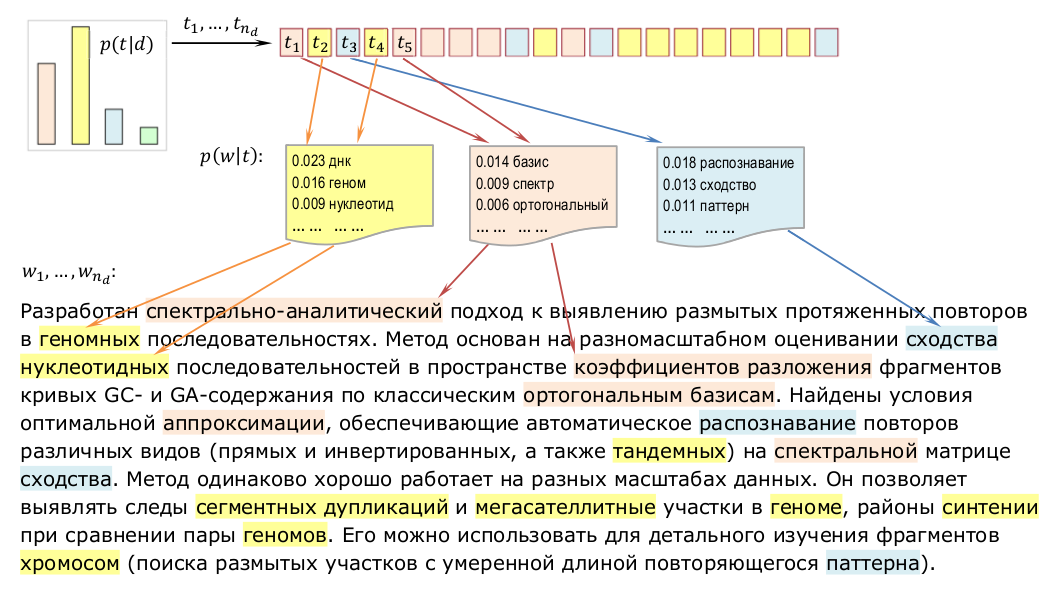
\includegraphics[scale=0.45]{img/te} 
			\caption{Пример выделения тем в тексте (\texttt{ru.wikipedia.org/wiki/Темат
			ическое\_моделирование}).}
			\label{pic1}
	\end{figure}

	\begin{figure}
			\centering 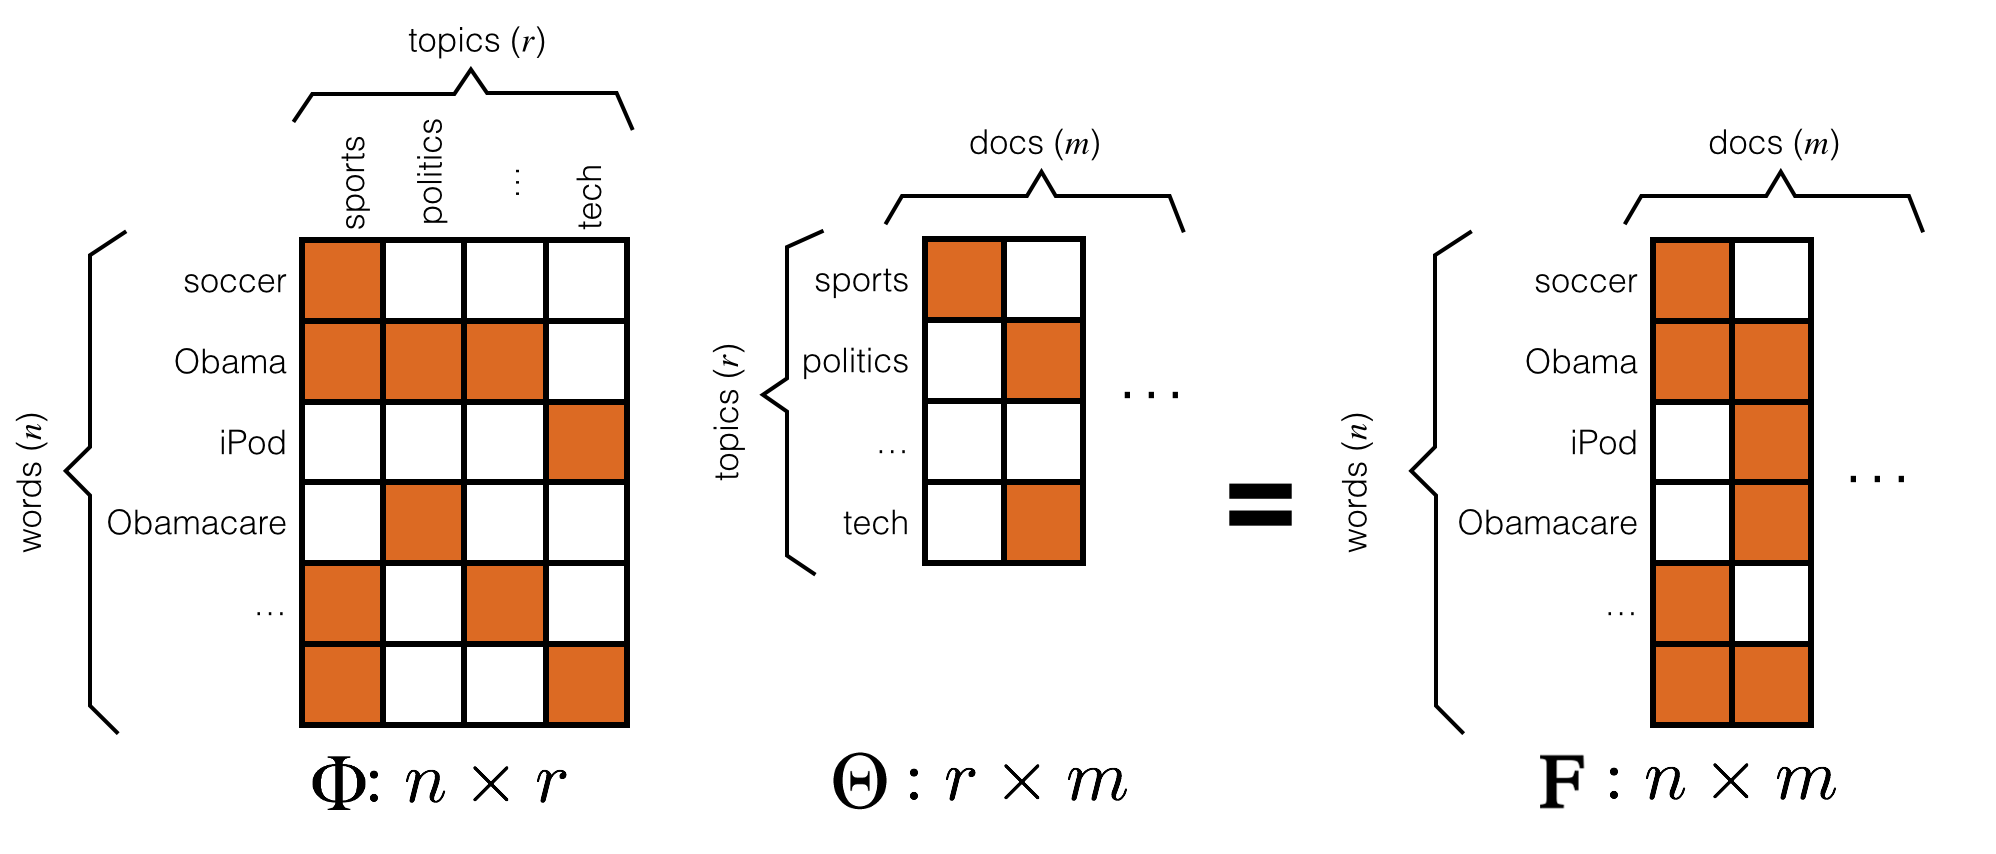
\includegraphics[scale=0.25]{img/tm} 
			\caption{Пример записи тематической модели в матричной форме \cite{CatalinVoss14}}
			\label{pic2}
	\end{figure}
   	
   	\subsection{Предобработка коллекции}
   	\label{pros_coll}
   	Предобработка коллекции предполагает удаление <<лишней>> информации, которая, как предполагает исследователь, негативно сказывается на качестве модели. 
   	
   	Избыточное количество параметров модели, как правило, влечёт за собой переобучение и медленную настройку модели. Именно поэтому большинство преобразований направлены на уменьшение параметров тематической модели, обычно за счёт уменьшения размера словаря. Некоторые примеры популярных преобразований:
   	\begin{itemize}
   		\item На основе предположения, что редкие термины не могут быть яркими представителями какой-либо темы, производят удаление редких терминов, что существенно сокращает размер коллекции, потому что редкие термины составляют $85-90\%$ словаря коллекции. Уменьшение словаря положительно сказывается на метриках качества модели. В то же время такое преобразование усугубляет проблему полноты, повышает количество незнакомых модели слов. 
   		\item На основе предположения, что разные формы одного и того же термина не влияют на тематическую окраску, термины приводят к нормальной форме, что так же уменьшает словарь модели. Процесс нормализации позволяет убрать из исходного текста грамматическую информацию (падежи, числа, глагольные виды и времена, залоги причастий, род и так далее), оставляя смысловую составляющую.
   		\item На основе  предположения, что некоторые части речи (междометия, предлоги, союзы, частицы, местоимения) не несут в себе тематическую окраску, с целью уменьшения размера словаря и коллекции, слова таких частей речи можно удалить.
   		\item На основе предположения, что термины общей лексики (стоп-слова) не несут в себе тематической окраски, их также можно удалить.
   		\item Иногда предполагается, что из коллекции выделены словосочетания и добавлены в коллекцию, как уникальные элементы словаря. Обычно значение такого термина отлично от значений слов его образующих. К примеру \textit{Машина опорных векторов}, имеет посредственное отношение к \textit{машинам}, \textit{опорам} или \textit{векторам}. 
   		\item Пренебрегают знаками пунктуации и непечатными символами, приводят все термины к одному регистру.
   	\end{itemize}
   	
\subsection{Метрики качества}
	Задача тематического моделирования некорректно поставлена, в отличие от задач классификации или регрессии здесь нет чёткого понятия «ошибки» или «потери». Стандартные критерии качества кластеризации плохо подходят для оценивания «мягкой» совместной кластеризации документов и терминов. 
	
	Поэтому нет возможности предложить одну метрику, которая сможет дать полную информацию о качестве тематической модели. Из всех предложенных сообществом метрик, как правило, стандартом являются: перплексия и когерентность. 
	
 	\subsubsection*{Перплексия}
 	Наиболее распространённым критерием является перплексия (perplexity), используемая для оценивания моделей языка в компьютерной лингвистике. Это мера несоответствия или «удивлённости» модели $p(w | d)$ терминам w, наблюдаемым в документах d коллекции D, определяемая через логарифм правдоподобия:
	\begin{equation}
	 	LogLikelyHood(D, \Phi, \Theta) = \sum_{d \in \mathrm{D}} \sum_{w \in d} n_{dw}~ln \sum_{t \in T} \phi_{wt} \theta_{td}
		\label{llh}
	\end{equation}
 	\begin{equation}
	 	Perplexity(D, \Phi, \Theta) = exp\left( -\frac{1}{len(\textrm{D})}~LogLikelyHood(D, \Phi, \Theta) \right)
	 	\label{perp}
	\end{equation}
 	
 	Чем меньше эта величина, тем лучше модель p предсказывает появление терминов $w$ в документах $d$ коллекции $\textrm{D}$. 
 	
 	Перплексия чувствительна к размеру словаря, что делает её неприменимой для сравнения тематических моделей с различным словарём. Эта проблема решена в \cite{Nyzhybytskyy}. 
 	
 	Поскольку перплексия определена через правдоподобие, то величина перплексии сама по себе не несёт информации о качестве модели, но сравнивать перплексии разных моделей --- корректно.
 	\subsubsection*{Когерентность}
 	Когерентность (coherence) -- мера интерпретируемости тем, предложенная в \cite{Newman09}. Когерентность показала высокую корреляцию с оценками экспертов. 
 	\begin{equation}
	 	Coherence(D,~Topic) = median\left(log\frac{P(w_1, w_2)}{P(w_1) P(w_2)}:~w_i, w_j\in Topic_{1, \dots, 10}\right)
 		\label{ch}
 	\end{equation}

 	На самом деле, с точки зрения теории информации когерентность является поточечной взаимной информацией. Чем эта метрика больше, тем тема более интерпретируема. В то же время высокая когерентность не гарантирует, что тема будет хорошей с точки зрения семантической связности, это значит, что когерентность необходимо использовать вместе с перплексией. Общая когерентность модели определятся как медиана когерентностей тем.
 	
 	\subsubsection*{Мера уникальности ядер}
 	Исходя из предположения, что темы выделенные человеком в коллекции как правило будут иметь уникальное ядро -- набор терминов с высокой вероятностью в данной теме. Мера уникальности ядер показывает насколько темы не похожи между собой. 
 	\begin{equation}
 		KernelsUniq = \frac{|uniq(kernels)|}{|kernels|}
	\label{uk}
	\end{equation}
 			
 	Чем уникальность ядер ближе к единице, тем легче различить темы, чем уникальность ближе к нулю, тем сложнее разделить темы. В данной работе ядро темы --- набор десяти наиболее вероятных терминов в теме.

\newpage
\section{Алгоритмы тематического моделирования}
В данном разделе, приведен краткий обзор основных методов и подходов к решению задачи \emph{тематического моделирования}. Основным алгоритмом является PLSA (ARTM и PLSA-SIM являются его модификациями), существенно отличным от PLSA является алгоритм ANCHOR WORDS.

\subsection{PLSA}
	\textbf{Probabilistic Latent Semantic Analysis} (Вероятностный латентный семантический анализ, PLSA) был предложен Томасом Хофманном в \cite{Hofmann99}.
	
	Для построения модели, предполагается оптимизировать логарифм правдоподобия, одновременно с этим оптимизируя перплексию,
   	\begin{equation}
   	LogLikelyHood(D, \Phi, \Theta) = \sum_{d \in \mathrm{D}} \sum_{w \in d} n_{dw}~ln \sum_{t \in T} \phi_{wt} \theta_{td} \rightarrow \max_{\Phi,\Theta},
   	\end{equation}
   	
   	при ограничениях нормировки и неотрицательности \ref{smd_norm}.
   	
   	Для решения поставленной оптимизационной задачи предлагается использовать EM-алгоритм, используемый в математической статистике для нахождения оценок максимального правдоподобия параметров вероятностных моделей, в случае, когда модель зависит от некоторых скрытых переменных, каждая итерация которого состоит из двух шагов~--~Expectation, Maximization.  
   	
   	На E-шаге по текущим значениям параметров $\phi_{wt}$, $\theta_{td}$ с помощью формулы Байеса вычисляются условные вероятности $p(t| d, w)$ всех тем $t \in T$ для каждого термина $w \in d$ в каждом документе d:
   	
   	\begin{equation}
   	H_{dwt} = p(t|d, w) = \frac{p(w|t)p(t|d)}{p(w|d)} = \frac{\phi_{wt} \theta_{td}}{\sum_{t' \in T}\phi_{wt'}\theta_{t'd}}
   	\end{equation}
   	
   	На M-шаге, наоборот, при фиксированных вероятностях тем $H_{dwt}$ вычисляются оценки максимального правдоподобия для параметров $\phi_{wt}$,~$\theta_{td}$:
   	\begin{equation}\phi_{wt} = \frac{n_{wt}}{n_t},~~~~~~~~~~~~n_{wt} = \sum_{d \in D} n_{dw}H_{dwt},~~~~~~~~~~~~n_t = \sum_{w \in W} n_{wt}\end{equation}
   	\begin{equation}\theta_{td} = \frac{n_{dt}}{n_d},~~~~~~~~~~~~n_{dt} = \sum_{w \in d} n_{dw}H_{dwt},~~~~~~~~~~~~n_d = \sum_{t \in T} n_{td}\end{equation}
   	Перед началом работы алгоритма необходимо задать начальное приближение $\Phi$ и $\Theta$, что можно сделать нормированными случайными векторами. Но на самом деле выбор хорошего начального приближения является отдельной сложной задачей. 
   	
   	Более того, PLSA достаточно чувствителен к выбору начального приближения~---~изменяя только начальное приближение можно получить существенно различные темы и качество модели.
   
   	\begin{singlespacing}
   		\begin{algorithm}
   		\caption{EM-алгоритм для тематической модели PLSA.}
   		\label{plsa}
   			\textbf{Вход}: коллекция $\textrm{D}$, число тем $|\textrm{T}|$, начальные приближения $\Phi$ и $\Theta$; \\
   			\textbf{Выход}: распределения $\Phi$ и $\Theta$; 
   		\begin{algorithmic}[1]
   			\Repeat
   				\State обнулить $n_{wt}$, $n_{dt}$, $n_{t}$ для всех $d \in \mathrm{D},~w \in \mathrm{W},~t \in \mathrm{T}$
   				\ForAll{$d \in \mathrm{D},~w \in d$:} 
   					\State $Z = \sum_{t \in \mathrm{T}} \phi_{wt} \theta_{td}$;
   					\ForAll{ $t \in \mathrm{T}$ таких, что $\phi_{wt}\theta_{td} > 0$}:
   					\State увеличить $n_{wt}$, $n_{dt}$, $n_t$ на $\delta = n_{dw} \phi_{wt}\theta_{td}/Z$;
   					\EndFor
   				\EndFor
   				\State $\phi_{wt} = n_{wt}/n_t$ для всех $w \in \mathrm{W},~t \in \mathrm{T};$
				\State $\theta_{td} = n_{td}/n_d$ для всех $d \in \mathrm{D},~t \in  \mathrm{T};$
   			\Until{$\Phi$ и $\Theta$ не стабилизируются}
   		\end{algorithmic}
   		\end{algorithm}
   	\end{singlespacing}
   	
Сложность по времени EM-алгоритма \ref{plsa} для решения задачи PLSA, $\mathit{O} (Iter \cdot \mathrm{T} \cdot [len(\mathrm{D})+\mathrm{W}+ \mathrm{D}])$, сложность по памяти зависит от эффективности хранения матриц $\Phi,~\Theta$, и в самом худшем случаи составляет $\mathit{O}(\textrm{T}(\textrm{W}+\textrm{D}))$.

\subsubsection*{Аддитивная регуляризация тематических моделей}
Задачи матричного разложения, как правило нуждаются в регуляризации, чтобы избежать переобучения, в свою очередь регуляризация может как быть совершенно искусственной, к примеру как распределение Дирихле в модели <<Латентное размещение Дирихле>> (latent Dirichlet
allocation, LDA)\cite{Blei03}, так и нести в себе лингвистический смысл как <<Аддитивная регуляризация тематических моделей, АРТМ>> \cite{ARTM}.

В работах \cite{ARTM, Voron13, Voron15slides} предложена теория АРТМ. В приведённых работах предложены регуляризаторы, направленные на выполнение некоторых лингвистически требований к строению тематической модели: разреживание, сглаживание, декорреляция тем и другие. Причём записывать такие регуляризаторы можно не прибегая к использованию теории \emph{Байесовского вывода}, что во многом упрощает и ускоряет разработку новых регуляризаторов.

С помощью аддитивной регуляризации (комбинации нескольких регуляризаторов), были устранены многие недостатки PLSA.

\subsubsection*{Учёт сходства между униграммами и биграммами}
Оригинальные тематические модели (PLSA и LDA) используют модель \emph{мешка слов}, предполагающую независимость слов друг от друга. Однако в документах есть много слов, связанных между собой по смыслу, в частности однокоренных, например: банк -- банковский -- банкир, кредит -- кредитный -- кредитовать -- кредитование и др.

В работе \cite{Nokel} предложена техника (модификация PLSA) учёта в тематических моделях похожих униграм и биграмм, с помощью которой было получено значительное улучшение метрик качества модели.

   	
\subsection{Алгоритм Anchor Words}
Известно, что для невыпуклых функций задача поиска глобального экстремума является NP-полной \cite{Kreinovich05}, поэтому возникает вопрос, можно ли решить задачу \ref{tmtask} не прибегая к принципу максимума правдоподобия.

В работе \cite{Arora12} был предложен алгоритм Anchor Words при наличии некоторых условий решающий задачу \ref{tmtask} за полиномиальное время, но фактическая сложность была очень высокой, настолько, что предложенный алгоритм был неприменим на практике. 

Алгоритм, приведённый в \cite{Arora12}, решает многочисленные линейные задачи, а также требует наложения определённых ограничений на искомые темы, использует построение обратных матриц, что приводит к неустойчивости алгоритма и возможности появления отрицательных вероятностей в  стохастических матрицах.

После чего в статье \cite{Arora12b} был предложен модифицированный алгоритм Anchor Words, дана простая интерпретация <<якорного разложения>> и так же были предложены некоторые не столь значительные оптимизации алгоритма Anchor Words.

В итоге алгоритм оказался в значительно быстрее, чем PLSA-подобные алгоритмы и не унаследовал проблему с выбором начального приближения.

\subsubsection*{Основная идея алгоритма Anchor Words}
Если в матрице $\Phi$ для каждой темы существует слово, которое только в этой теме имеет ненулевую вероятность большую чем $p$, то будем называть такую матрицу p-разделимой (Рис.~\ref{psep}).  

	\begin{figure}
			\centering 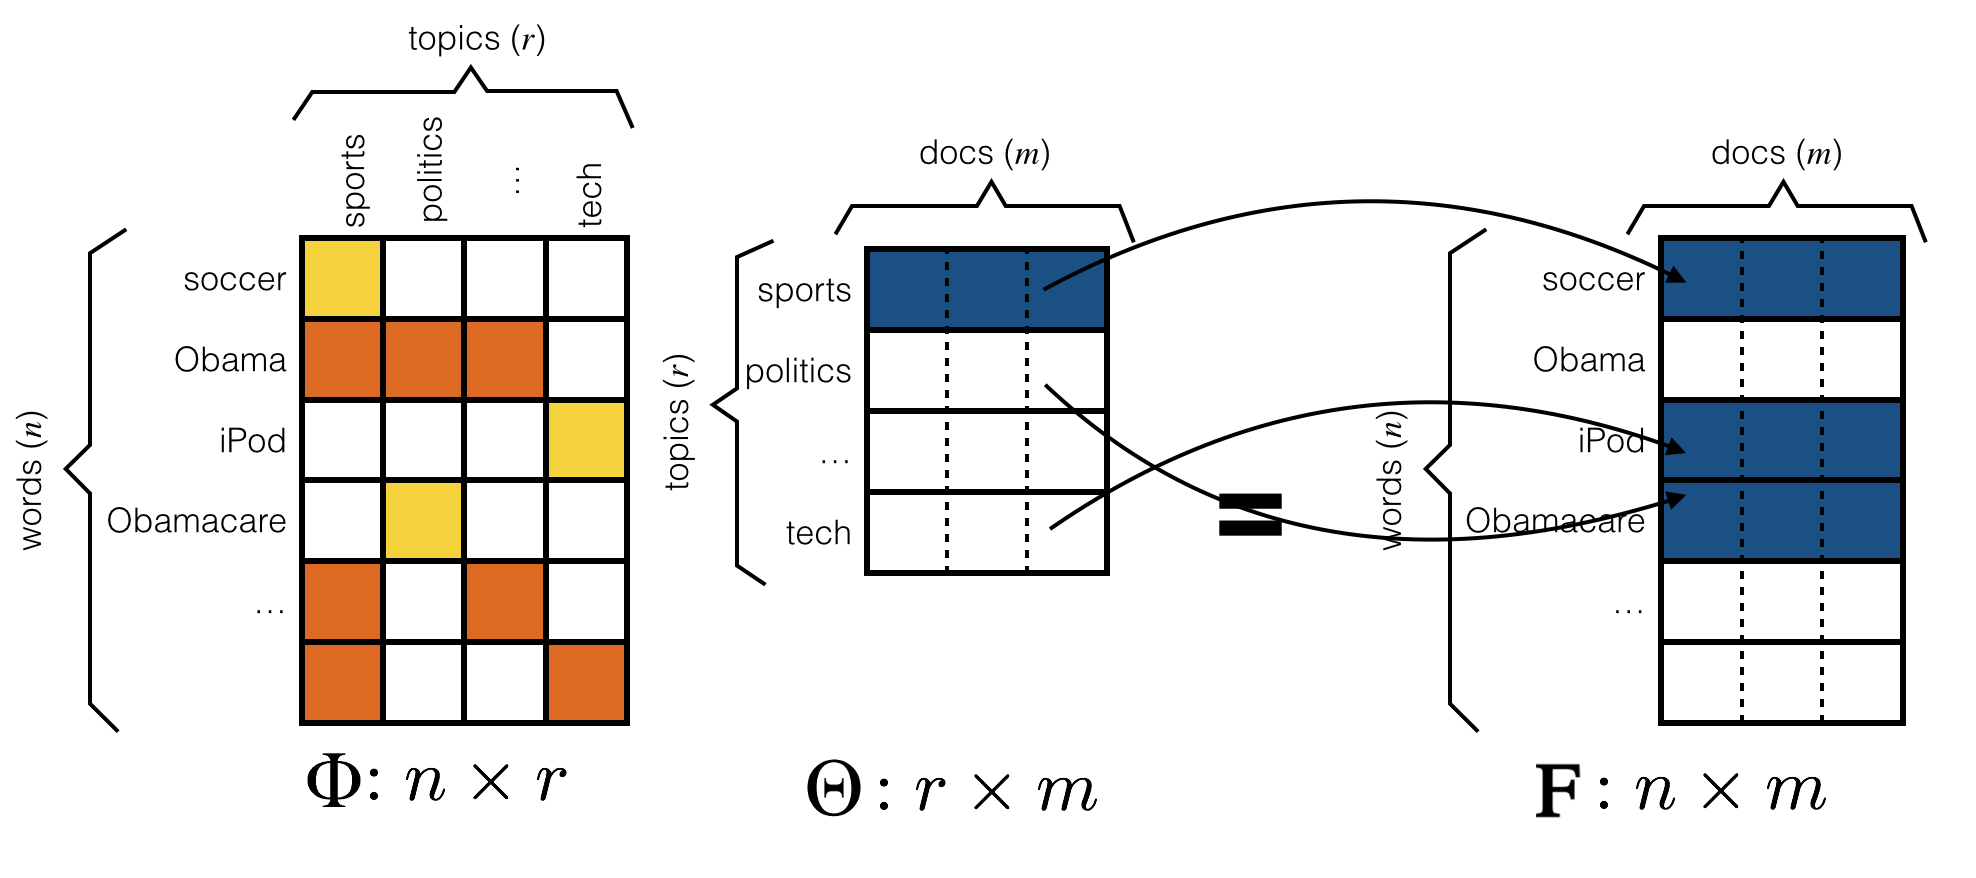
\includegraphics[scale=0.25]{img/psep} 
			\caption{p-разделимая матрица, \cite{CatalinVoss14}}
			\label{psep}
	\end{figure}

Пусть матрица $\Phi$ --- p-разделима, тогда в матрице $F$ существуют строки, которые являются масштабированными копиями строк из $\Theta$ (Рис.~\ref{anch_1}). Будем называть такие строки <<якорными>>.
	\begin{figure}
			\centering 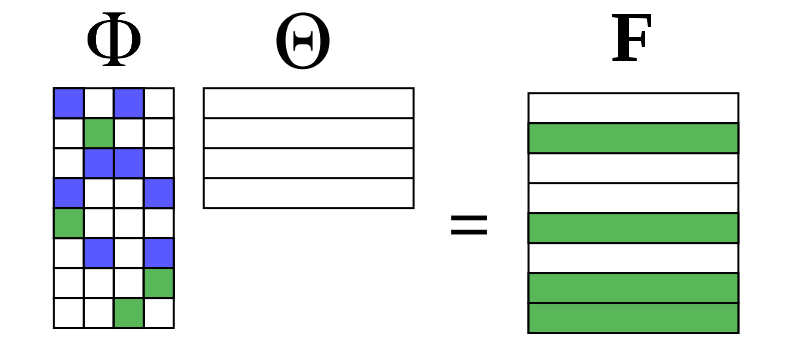
\includegraphics[scale=0.5]{img/anch_1} 
			\caption{p-разделимая матрица, \cite{AnkurMoitraSlides}.}
			\label{anch_1}
	\end{figure}
Причём, из свойств матричного перемножения все остальные строки матрицы $F$ являются линейной комбинация якорных строк \cite{Arora12}.

Каждая <<якорная>> строка соответствует некоторой теме, и набор <<якорных>> строк является базисом, откуда логично получить разложения строк-векторов остальных слов по якорным (базисным) строкам (Рис.~\ref{anch_2}). 
	\begin{figure}[h]
		\centering 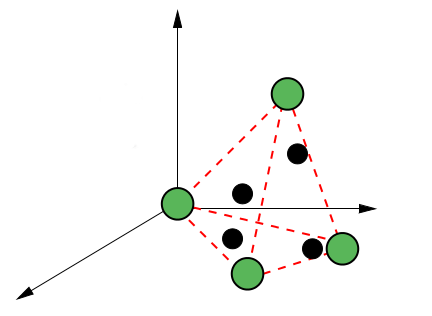
\includegraphics[scale=0.6]{img/anch_2} 
		\caption{Разложения по якорным словам, \cite{AnkurMoitraSlides}.}
		\label{anch_2}
	\end{figure}
Якорные слова можно получить как выпуклую оболочку строк матрицы $F$. 

Но есть проблема, вместо матрицы $F$ мы имеем приближение $\hat{F}$ которая на практике не устойчива и может плохо аппроксимировать $F$ (Рис.~\ref{anch_3}) \cite{Arora12}. 
\begin{figure}[h]
		\centering 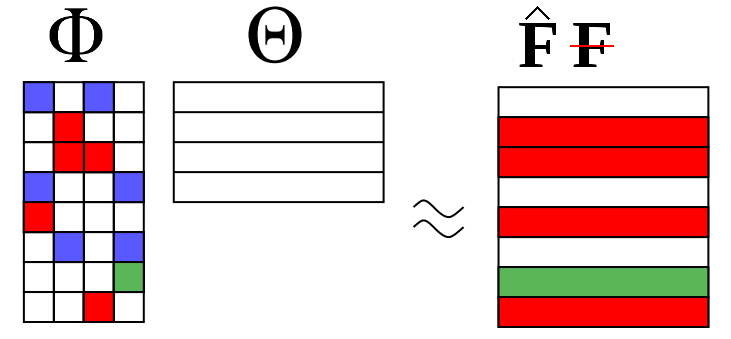
\includegraphics[scale=0.5]{img/anch_3} 
		\centering 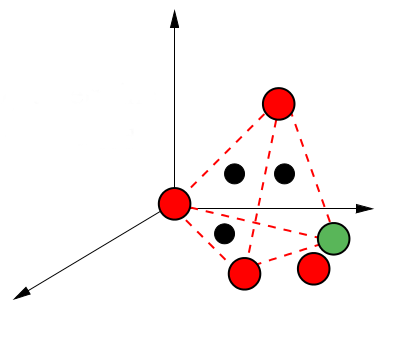
\includegraphics[scale=0.5]{img/anch_4}
		\caption{Неустойчивость матрицы $F$, \cite{AnkurMoitraSlides}.}
		\label{anch_3}
\end{figure}

В \cite{Arora12} было предложено, использовать вместо матрицы $\hat{F}$ матрицу $FF^t$ (Рис.~\ref{anch_4}), 

\begin{equation}
	\hat{F}\hat{F}^t \rightarrow FF^t.
\end{equation}


К счастью, то же свойство линейной комбинации строк сохраняется и для $FF^t$. Поэтому возможно восстановить якорные слова из $FF^t$. Так же заметим, что $\Theta \Theta^t \rightarrow R$, $R_{\mathrm{T} \times \mathrm{T}}$ можно рассматривать как ковариационную матрицу тем. 

   	\begin{singlespacing}
   		\begin{algorithm}
   		\caption{Высокоуровневый алгоритм Anchor Words.}
   		\label{plsa}
   			\textbf{Вход}: коллекция $\textrm{D}$, число тем $|\textrm{T}|$\\
   			\textbf{Выход}: матрица $\Phi$; 
   		\begin{algorithmic}[1]
   				\State $Q$ = Word Co-occurences($\textrm{D}$)
   				\State $\hat{Q}$ = Rows normalized $Q$
   				\State $S$ = FindAnchorWords($\hat{Q}$, $|\textrm{T}|$)
   				\State $\Phi$ = RecoverWordTopic($\hat{Q}$, $S$)
   				\State \Return $\Phi$
   		\end{algorithmic}
   		\end{algorithm}
   	\end{singlespacing} 
Ковариационную матрицу тем, наглядно, можно представить следующим образом \ref{anch_4}.   	
\begin{figure}[h]
		\centering 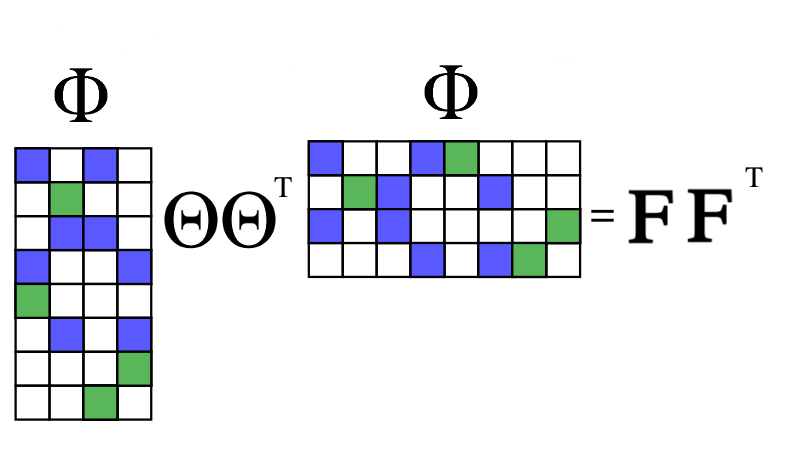
\includegraphics[scale=0.45]{img/anch_5}  
		\caption{Матрица $FF^t$ до переупорядочивания строк (столбцов) в $\Phi, \Theta$, \cite{AnkurMoitraSlides}.}
		\label{anch_4}
\end{figure}

\subsubsection*{Алгебраический подход к использованию p-разделимости}
В этом разделе необходимо понять, как можно использовать р-разделимость и якорные слова для поиска матриц $\Phi$ и $\Theta$.

В \cite{Arora12} приведён алгоритм решающий эту задачу. Переупорядочим строки и столбцы матрицы $F$, так, чтобы якорные строки и столбцы стояли в верхнем левом углу Рис. \ref{anch_6}.

\begin{figure}
		\centering 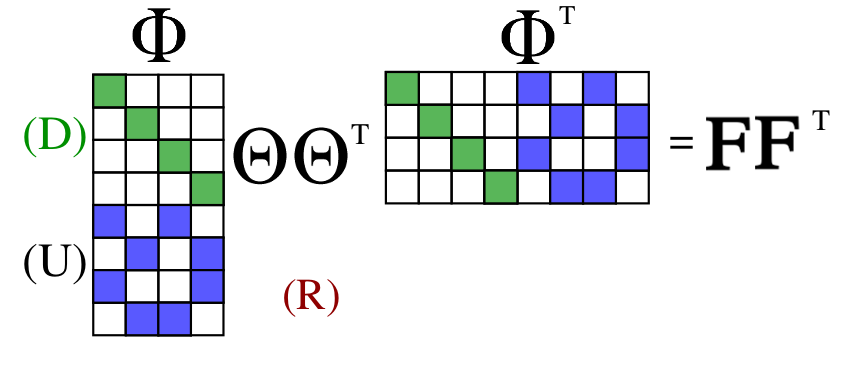
\includegraphics[scale=0.45]{img/anch_6} 
		\caption{Матрица $FF^t$ после переупорядочивания строк (столбцов) в $\Phi, \Theta$, \cite{AnkurMoitraSlides}, \cite{Arora12}.}
		\label{anch_6}
\end{figure}
 
По правилам блочного перемножения матриц
 	\begin{equation}
		Q = F\hat{F}^t = \Phi R \Phi^t= \begin{pmatrix}
		D\\
		U\end{pmatrix} R \begin{pmatrix}
		D & U^t\end{pmatrix}= \begin{pmatrix}
		DRD & DRU^t\\
		URD & URU^t
		\end{pmatrix},
 	\label{bm}
 	\end{equation}
тогда требуется решить следующую задачу -- по блокам, образующим матрицу $Q$, найти матрицы $D, U$.



   	\begin{singlespacing}
   		\begin{algorithm}
   		\caption{Алгебраический алгоритм RecoverWordTopic.}
   		\label{plsa}
   			\textbf{Вход}: матрица $Q$, множество якорных слов $S$\\
   			\textbf{Выход}: матрица $\Phi$; 
   		\begin{algorithmic}[1]
   				\State Переставим строки и столбцы в матрице $Q$, так чтобы якорные строки образовывали диагональную подматрицу.
   				\State $p_{S}$ = $Q_{S}\vec{1}$
   				\State $z$ = $solve_{z}(Q_{S,S}\cdot z = p_{S})$
   				\State $\Phi^t$ = $(Q_{S,S} \cdot Diag(\vec{z}))^{-1} \cdot Q_{S}^t$
   				\State \Return $\Phi$
   		\end{algorithmic}
   		\end{algorithm}
   	\end{singlespacing}
   	
Как уже было сказано ранее, этот алгоритм неприменим на практике.
\subsubsection*{Вероятностный подход к использованию p-разделимости}
В дополнение к недостаткам, описанным выше, хочется заметить, что алгебраический подход использует очень маленькую часть матрицы $F$, полагаясь только на совместную встречаемость  слов и якорных слов, а эта оценка может быть неточной, если какое либо слово встречается нечасто.
Заметим, что матрица $Q_{ij} = p(w_i, w_j)$ нормализованная по строкам может быть рассмотрена как матрица условных вероятностей $\bar{Q}_{ij} = p(w_i| w_j)$ \cite{Arora12b}. 

Обозначим множество индексов якорных слов как $S = \{s_1, \dots, s_t\}$. Якорные слова отличаются тем, что соответствующий набор строк из $\bar{Q}_{S}$ образуют выпуклую оболочку строк матрицы $\bar{Q}$.

Докажем это. заметим, что для якорных слов

\begin{equation}
	\bar{Q}_{S_t, j} = \sum_{t'} p(t'|s_t)\cdot p(w_j|t') 
	\label{anch_prob_1}
\end{equation}
\begin{equation}
	= p(w_j|t)
	\label{anch_prob_2}
\end{equation}

где \ref{anch_prob_1} верно в силу свойств матричного умножения, а \ref{anch_prob_2} потому, что $p(t| s_t)~=~1$. Для всех остальных слов
\begin{equation}
	\bar{Q}_{i, j} = \sum_{t'} p(t'| w_i)\cdot p(w_j| t') 
	\label{anch_prob_3}
\end{equation}

Обозначим вероятность $p(t| w_i)$ как $C_{i,t}$, тогда 

\begin{equation}
	\bar{Q}_{ij}~=~\sum_{t'} C_{i, t'} \bar{Q}_{s_{t'}j},~~\sum_{t'}C_{i, t'} = 1 	
\end{equation}

таким образом строки из Q являются линейной комбинацией якорных строк.

После чего пользуясь теоремой Байеса
\begin{equation}
p(w_i| t) = \frac{p(t| w_i)p(w_i)}{\sum_{i'} p(t| w_{i'})p(w_{i'})}
\end{equation}

можем восстановить матрицу $\Phi$.


 		\begin{algorithm}
 		\caption{Алгоритм RecoverWordTopic.}
 		\label{recwt}
 			\textbf{Вход}: Матрица $Q$, множество якорных слов $S$;\\
 			\textbf{Выход}: матрица $\Phi$; 
 		\begin{algorithmic}[1]
 				\State $\bar{Q} = row\_norm(Q)$
 				\State $p_w = Q \vec{1}$ \Comment{Сохраним нормировочные константы}
 				\ForAll $w \in \mathrm{W}$:
 					\State Решить задачу:
 					\begin{equation}
 						C_{i} = argmin_{\vec{C}_i} Measure(\bar{Q}_i,~~\sum_{t \in \mathrm{T} } C_{i, k}\cdot \bar{Q}_{s_k})
 						\label{task}
 					\end{equation}
			\State При ограничениях: $\sum_{t \in \mathrm{T} } C_{i, k} = 1, C_{ik} \geq 0$
 				\EndFor
		\State $A' = diag(\vec{p}_w)C$
		\State $A = col\_norm(A')$
		\State \Return A	
 		\end{algorithmic}
 		\end{algorithm}

   	
Если для решения оптимизационной задачи \ref{task} использовать метрику $L_2$
\begin{equation}
L_2(\bar{Q}_i,~C^t_i\bar{Q}_S) = \norm{\bar{Q}_i-C^t_i\bar{Q}_S}^2 = \norm{\bar{Q}_i}^2 - 2C_i(\bar{Q}_S \cdot \bar{Q}^t_i) + C^t_i(\bar{Q}_S\cdot\bar{Q}^t_S)C_i,
\end{equation}
то вычисление метрики на каждом шаге можно организовать независимо от размера словаря, поскольку $\bar{Q}_S\cdot\bar{Q}^t_S$ может быть посчитана только один раз и использоваться для всех слов, а $\bar{Q}_S \cdot \bar{Q}^t_i$ может так же быть вычислена только один раз, перед запуском алгоритма для слова $w_i$. 

\subsubsection*{Комбинаторный алгоритм для поиска якорных слов}
Комбинаторный алгоритм, представленный в \cite{Arora12b} приведён вместе с достаточно сложными математическими оценками, в работе будет приведён только сам алгоритм и приведены некоторые неформальные пояснения, оценки  корректности и времени работы будут опущены. 

При описании алгоритма $span(S)$ будет означать подпространство натянутое на вектора $S$.
Расстояние от точки $x$ до $span(S)$ вычисляется как норма проекции $x$ на ортогональное дополнение $span(S)$.

   		\begin{algorithm}
   		\caption{Комбинаторный алгоритм FastAnchorWords.}
   		\label{plsa}
   			\textbf{Вход}: Точки $V = {v_1, \dots, v_n}$, количество векторов для выпуклой оболочки -- $K$;\\
   			\textbf{Выход}: $\{v'_{1}, \dots, v'_{k}\}$ -- точки образующие наиболее выпуклую оболочку; 
   		\begin{algorithmic}[1]
   				\State Спроецировать $v_i$ на случайно выбранное пространство $V$,  $dim V = 4log V / \epsilon^2$
   				\State S = $\{s_0\}$, $s_0$ -- наиболее удалённая точка от начала координат.
   				\ForAll i=1 to K:
   				\State Обозначим $s_i$ точку из V наиболее удалённую от $span(S)$.
   				\State $S = S \cup \{s_i\}$
   				\EndFor
				\ForAll i=1 to K:
				\State Обозначим $s'_i$ точку из V наиболее удалённую от $span(S\setminus\{s_i\})$.
				\State Заменить $s_i$ на $s'_i$
				\EndFor
				\Return  S
   		\end{algorithmic}
   		\end{algorithm}
   	
Поскольку число векторов в $V$ равно его размерности необходимо снизить размерность пространства, уменьшение размерности позволяет избежать переобучения, уменьшить вычислительную сложность алгоритма.


\subsection{Недостатки стандартных алгоритмов}
\begin{enumerate}
\item Бедная модель документа -- модель \emph{мешка слов}, не учитывает совместную встречаемость слов, структуру предложений документа, в следствие чего теряет очень много информации.
\item Не используются даже простые предположения о структуре тематически окрашенных терминов -- высокую вероятность в теме может получить совершенно любой термин, так как при построении модели алгоритм руководствуется только частотами слов, но никак не учитывает их лексическую или грамматическую структуру.
\item Все модели, основанные на модели PLSA, неустойчивы к выбору начального приближения.
\item Модель Anchor Words, как правило, обладает более высокой, перплексией чем PLSA.
\end{enumerate}

\newpage
\section{Реализация}
\subsection{Используемые инструменты}
Для реализации тематических моделей был использован язык {\tt python}, в настоящее время {\tt python} (\href{https://www.python.org/download/releases/2.7/}{https://www.python.org/download/releases/2.7/}) является наиболее используемым языком общего назначения для проведения научных исследований. 

За исключением стандартных библиотек, были использованы следующие пакеты (\href{https://pypi.python.org/pypi/pip}{https://pypi.python.org/pypi/pip}): 

\begin{enumerate}
\item \texttt{ipython notebook} --- современная интерактивная среза для программирования. 
\item \texttt{nltk} --- пакет для обработки естественного языка, содержит различные синтаксические и семантические анализаторы.
\item \texttt{scipy} --- реализация высокоуровневых математических операций (обработка разреженных матриц, методы оптимизации, \dots) 
\item \texttt{numpy} --- реализация низкоуровнивых математических операций, быстрая работа с матрицами и векторами.
\item \texttt{pymorphy} --- морфологический и семантический анализ для текстов на русском языке.
\end{enumerate}
Реализация экспериментов и алгоритмов доступна по адресу  \href{https://goo.gl/f8ZdcW}{goo.gl/f8ZdcW}. 

\subsection{Процесс построения тематической модели}
Процесс построения модели можно наглядно представить следующим образом (Рис. \ref{buildtm}): первым этапом происходит сбор коллекции, чаще всего из открытых источников, далее над коллекцией производятся преобразования описанные в разделе \ref{pros_coll}, далее по подготовленной коллекции строятся тематические модели, вычисляются метрики качества, далее результаты анализируются для подготовки новых экспериментов.

\begin{figure}[H]
		\centering 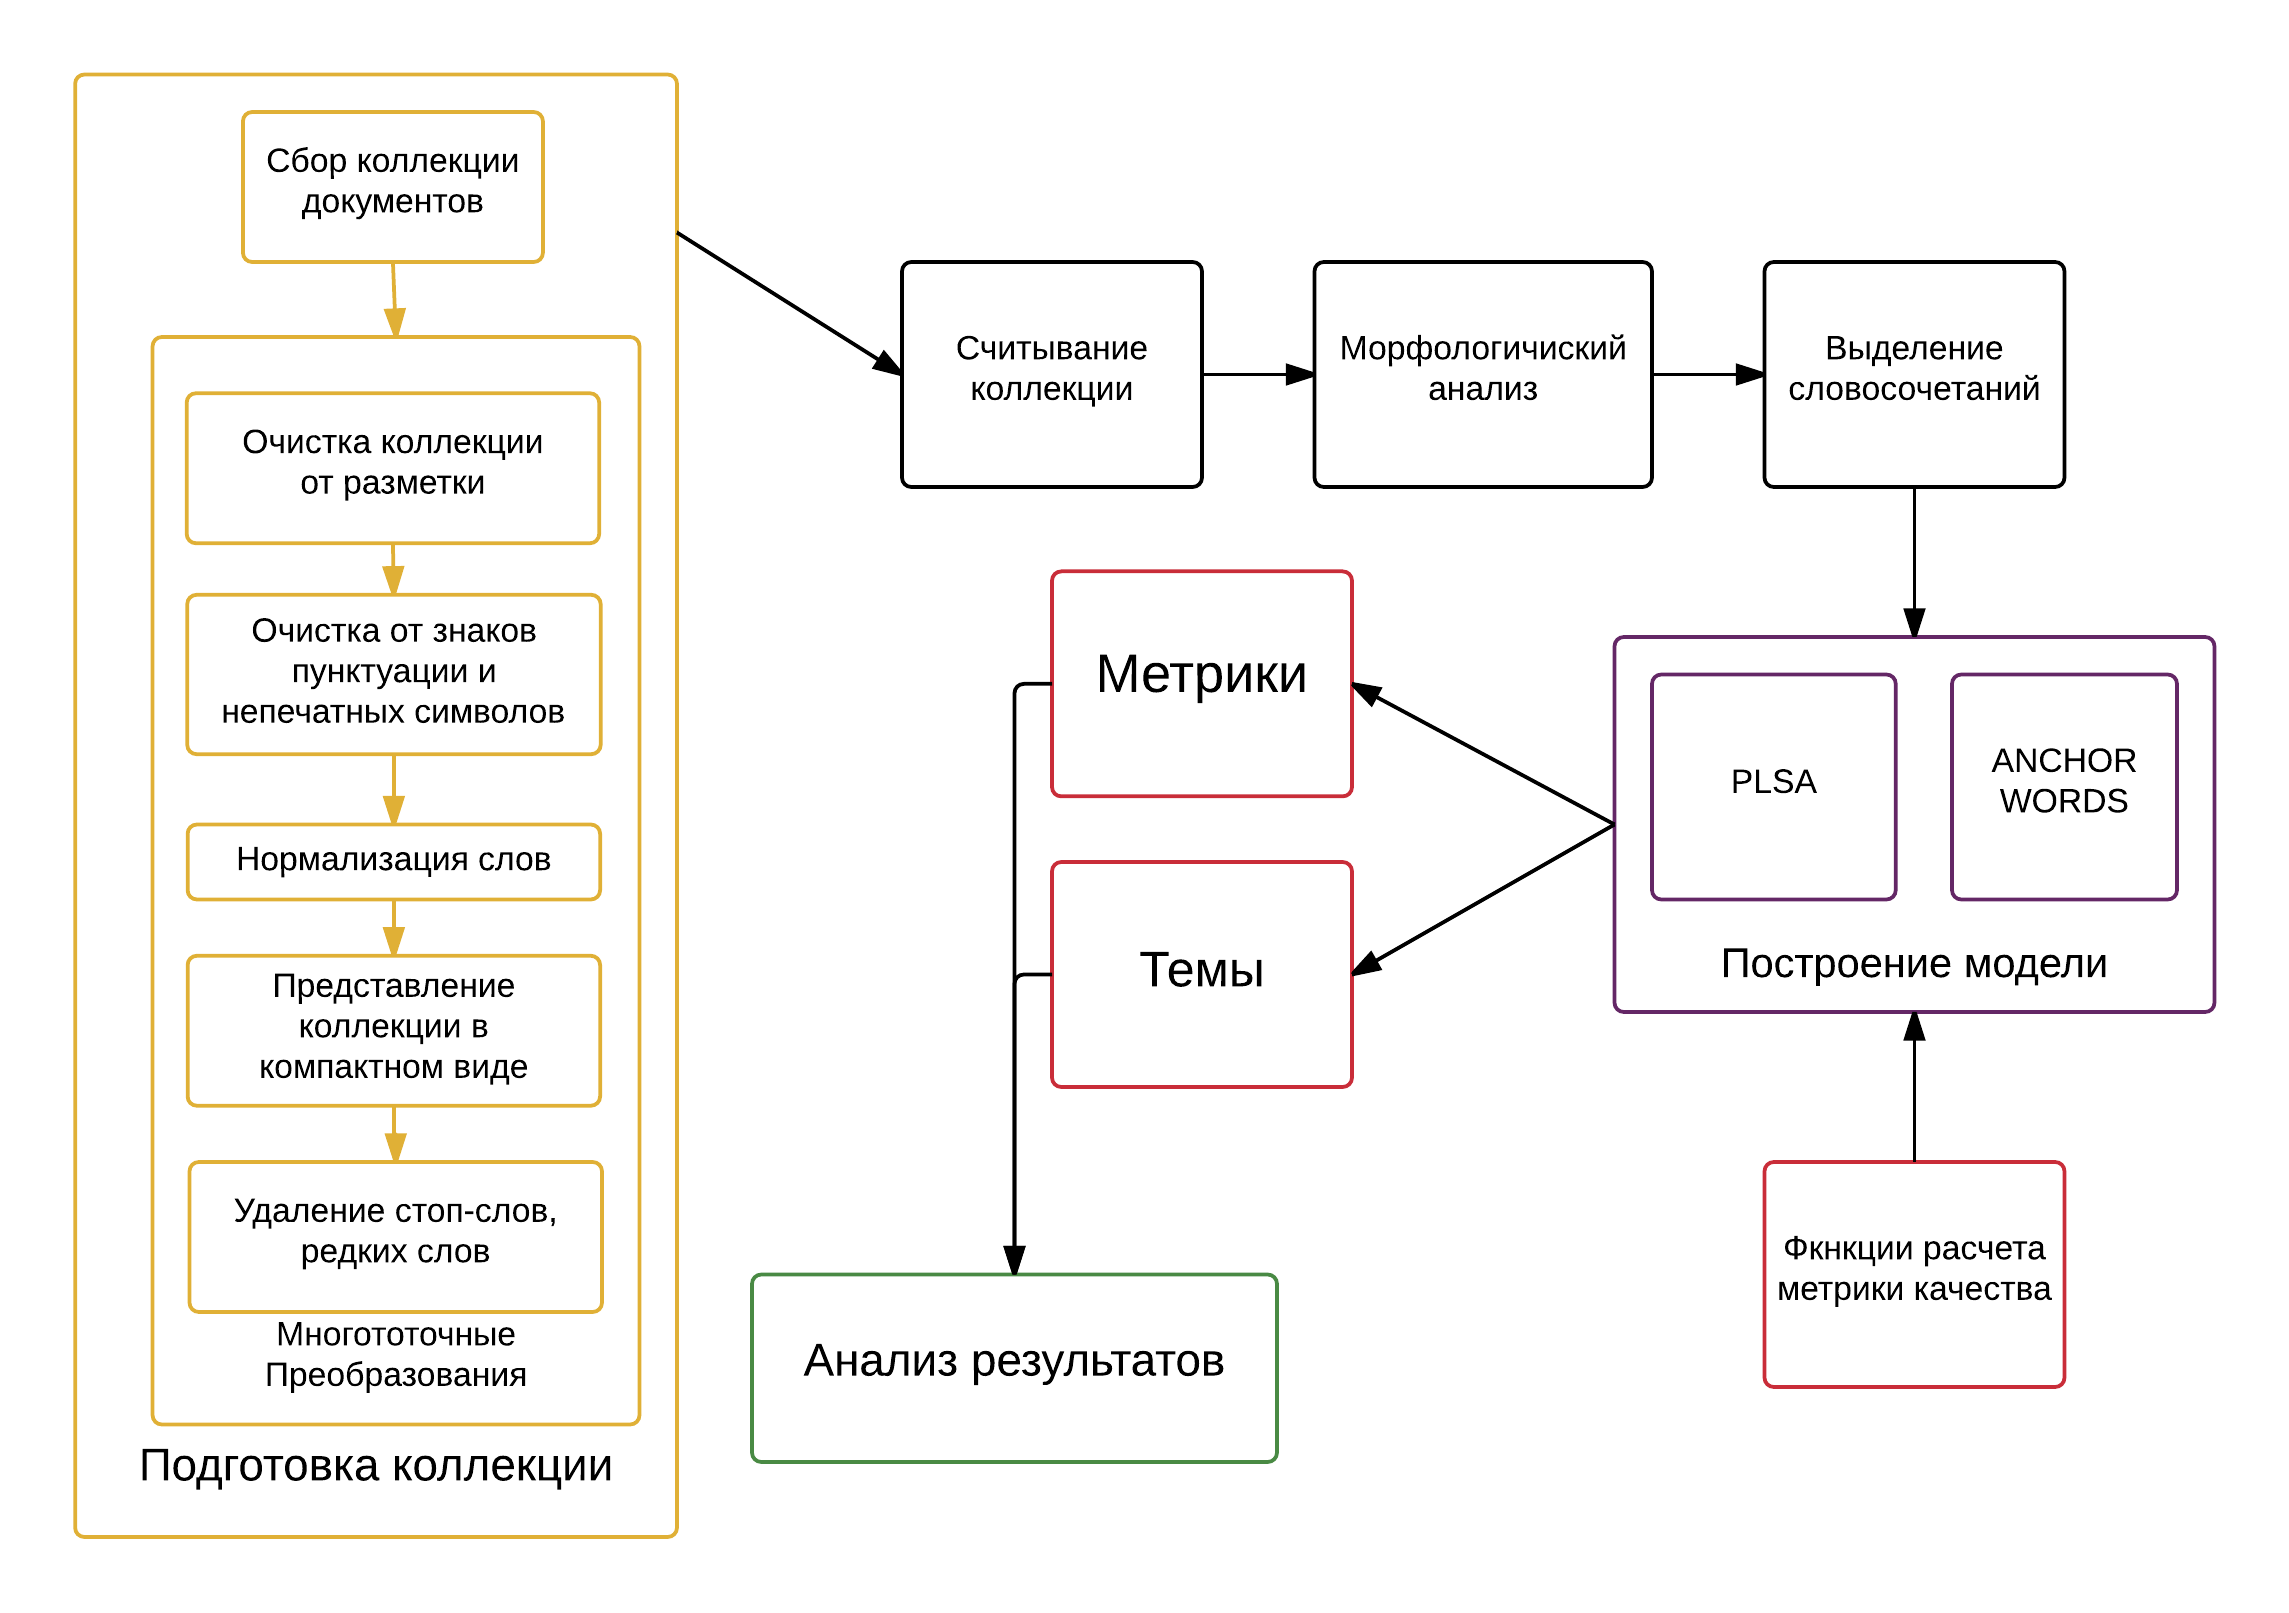
\includegraphics[scale=0.9]{img/pr}  
		\caption{Схема процесса построения тематической модели}
		\label{buildtm}
\end{figure}
\subsubsection*{Пример построения запуска эксперимента \\ для построения модели}

В приведенном листинге \ref{code1} приведен пример запуска алгоритма PLSA, на коллекции банковских статей. 

\begin{singlespace}
	\begin{mycode}{python}{Пример построения запуска эксперимента для построения модели}{code1}
import ...

collection = FullTextCollection(
    path='./tmtk/corpa/ru_bank_wid_small.zip', 
    lang='ru'
).fill()
    
F, T = plsa.plsa_model(
    collection, wrd_count=len(collection), 
    num_iter=40, verbose=True,
    metrics=[preplexity, coherence, uniq_top_of_topics])
plsa.print_topics(F, collection.id_to_words, 'res/pl.txt')
	\end{mycode}
	
\end{singlespace}


\newpage
\section{Учет лингвистических знаний \\ в тематических моделях}
\subsection{Постановка задачи}

Требуется разработать модификации стандартных моделей, с более высокой уникальностью ядер, засчёт интеграции дополнительных параметров: учета частей речи и словосочетаний. 

Реализовать данную модификацию и провести эксперименты и выполнить оценку качества моделей.


Цель данного раздела --- показать, что учёт лингвистических знаний может улучшить качество вероятностных тематических моделей, основанных только на частотах употребления слов.

Эксперименты, приведённые в данном разделе, проведены на коллекции текстов банковской тематики на русском языке, взятых из электронных журналов~ (\href{https://goo.gl/L97CZ8}{goo.gl/L97CZ8}). Предварительно слова в текстах были нормализованы, приведены к нижнему регистру. Было проведено удаление стоп-слов, тематически не окрашенных слов (по морфологическим характеристикам), знаков пунктуации.

Коллекция размером в 2500 документов была случайным образом разделена на 2000 документов для обучения и 500 для контроля.

Для вычисления \emph{перплексии} на тестовой коллекции документ случайным образом разделялся на две части (случайным образом выбирались слова из документа), после чего первая часть использовалась для оценки распределения тем в документе, а вторая для оценки перплексии.

Для представление результатов экспериментов использованы следующие обозначения:
\begin{enumerate}
	\item \texttt{an} --- алгоритм Anchor Words.
	\item \texttt{pl} --- алгоритм PLSA.
	\item \texttt{bi} --- использование словосочетаний, биграмм.
	\item \texttt{mr} --- использование морфологических ограничений.
	\item \textcolor{red}{1.23} --- нестабильный результат.
	\item \textbf{1.23} --- лучший результат.
\end{enumerate}

Результат для алгоритма выбирался фиксацией метрик на лучшей итерации, лучшей по перплексии на контроле (иногда почти самой лучшей в пределах двух итераций от лучшего значения).

Реализация экспериментов и алгоритмов доступна по адресу  \href{https://goo.gl/f8ZdcW}{goo.gl/f8ZdcW}. 

\subsection{Комбинация Anchor Words и PLSA}
\subsubsection*{Anchor Words как начальное приближение для PLSA}
	Алгоритмы Anchor Words и PLSA могут устранить недостатки друг друга: модель Anchor Words в отличии от PLSA не пользуется случайным приближением матриц $\Phi$ и $\Theta$, а руководствуется достаточно слабым предположением p-разделимости, модель PLSA оптимизирует перплексию, которая является недостатком Anchor Words.
	
	Возникает предположение, что модель Anchor Words будет хорошим  начальным приближением для PLSA. 
	
	Проведённые эксперименты подтвердили данное предположение одновременным улучшением сразу нескольких метрик качества. 
	
	Данное предположение уже обсуждалось в литературе, и не является идей автора, но дальнейшие эксперименты будут проведены именно с использованием комбинации моделей. 	
\subsubsection*{Эксперименты}

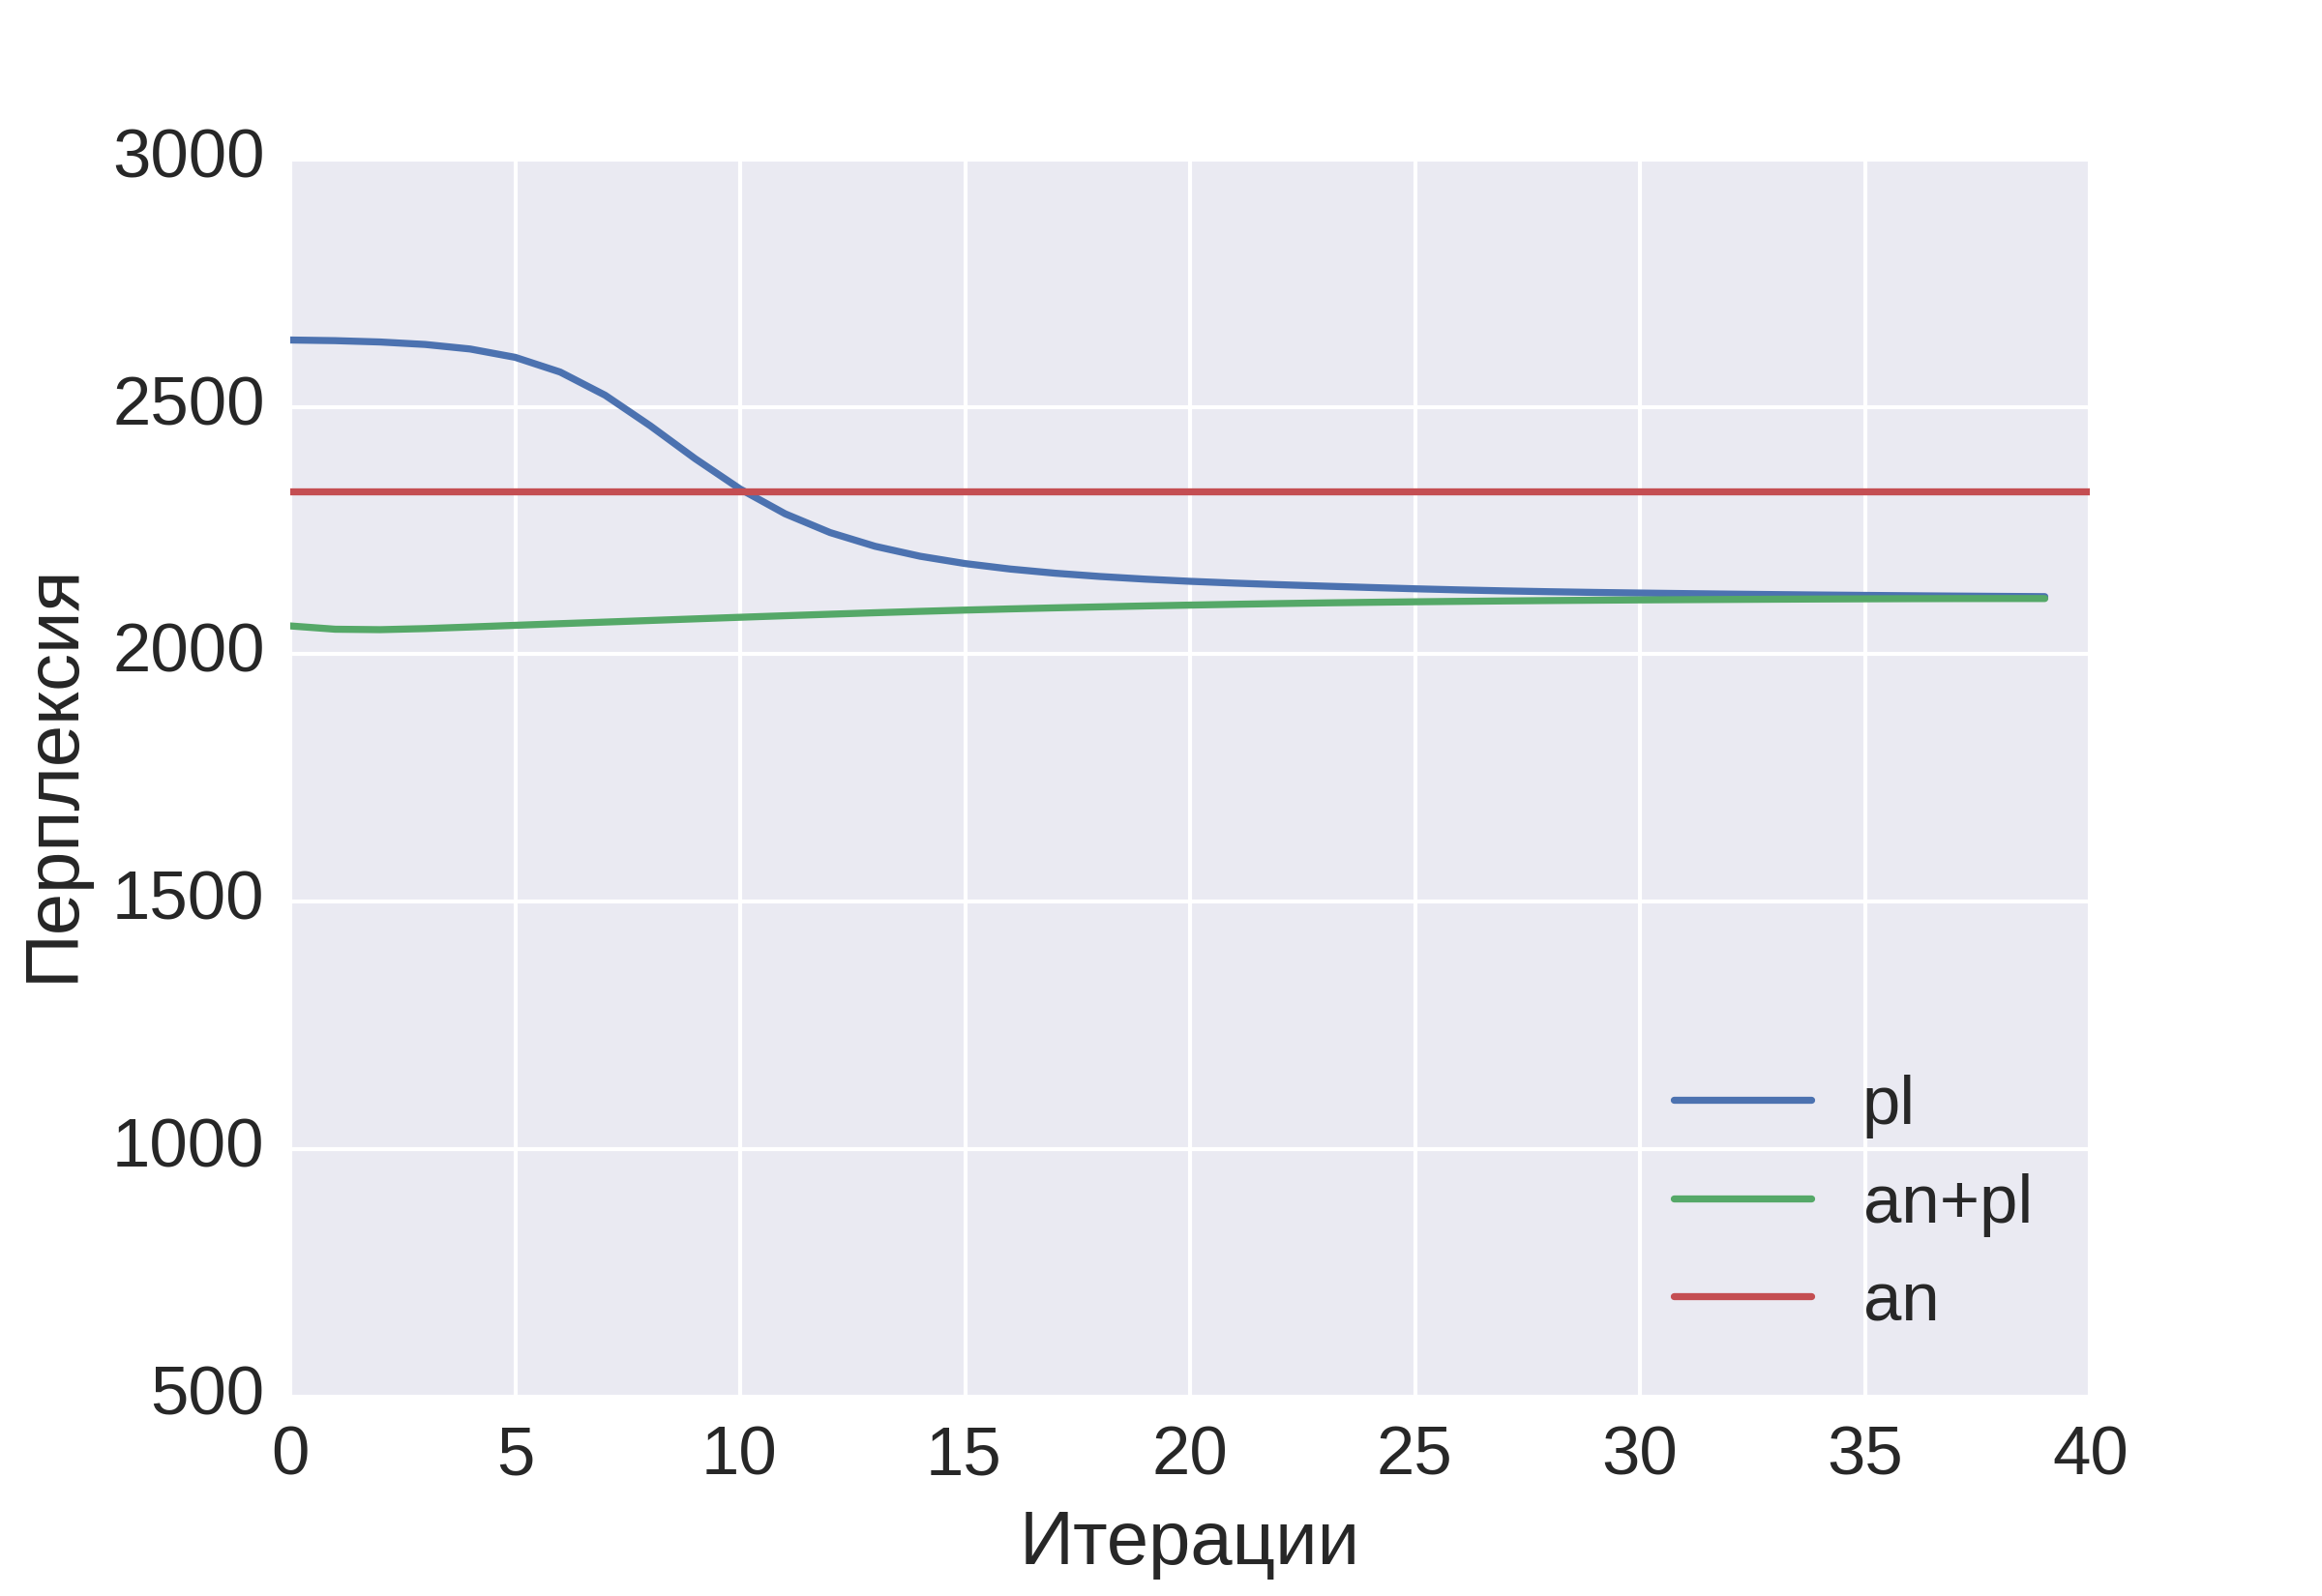
\includegraphics[scale=0.43]{img/anpl/1}  
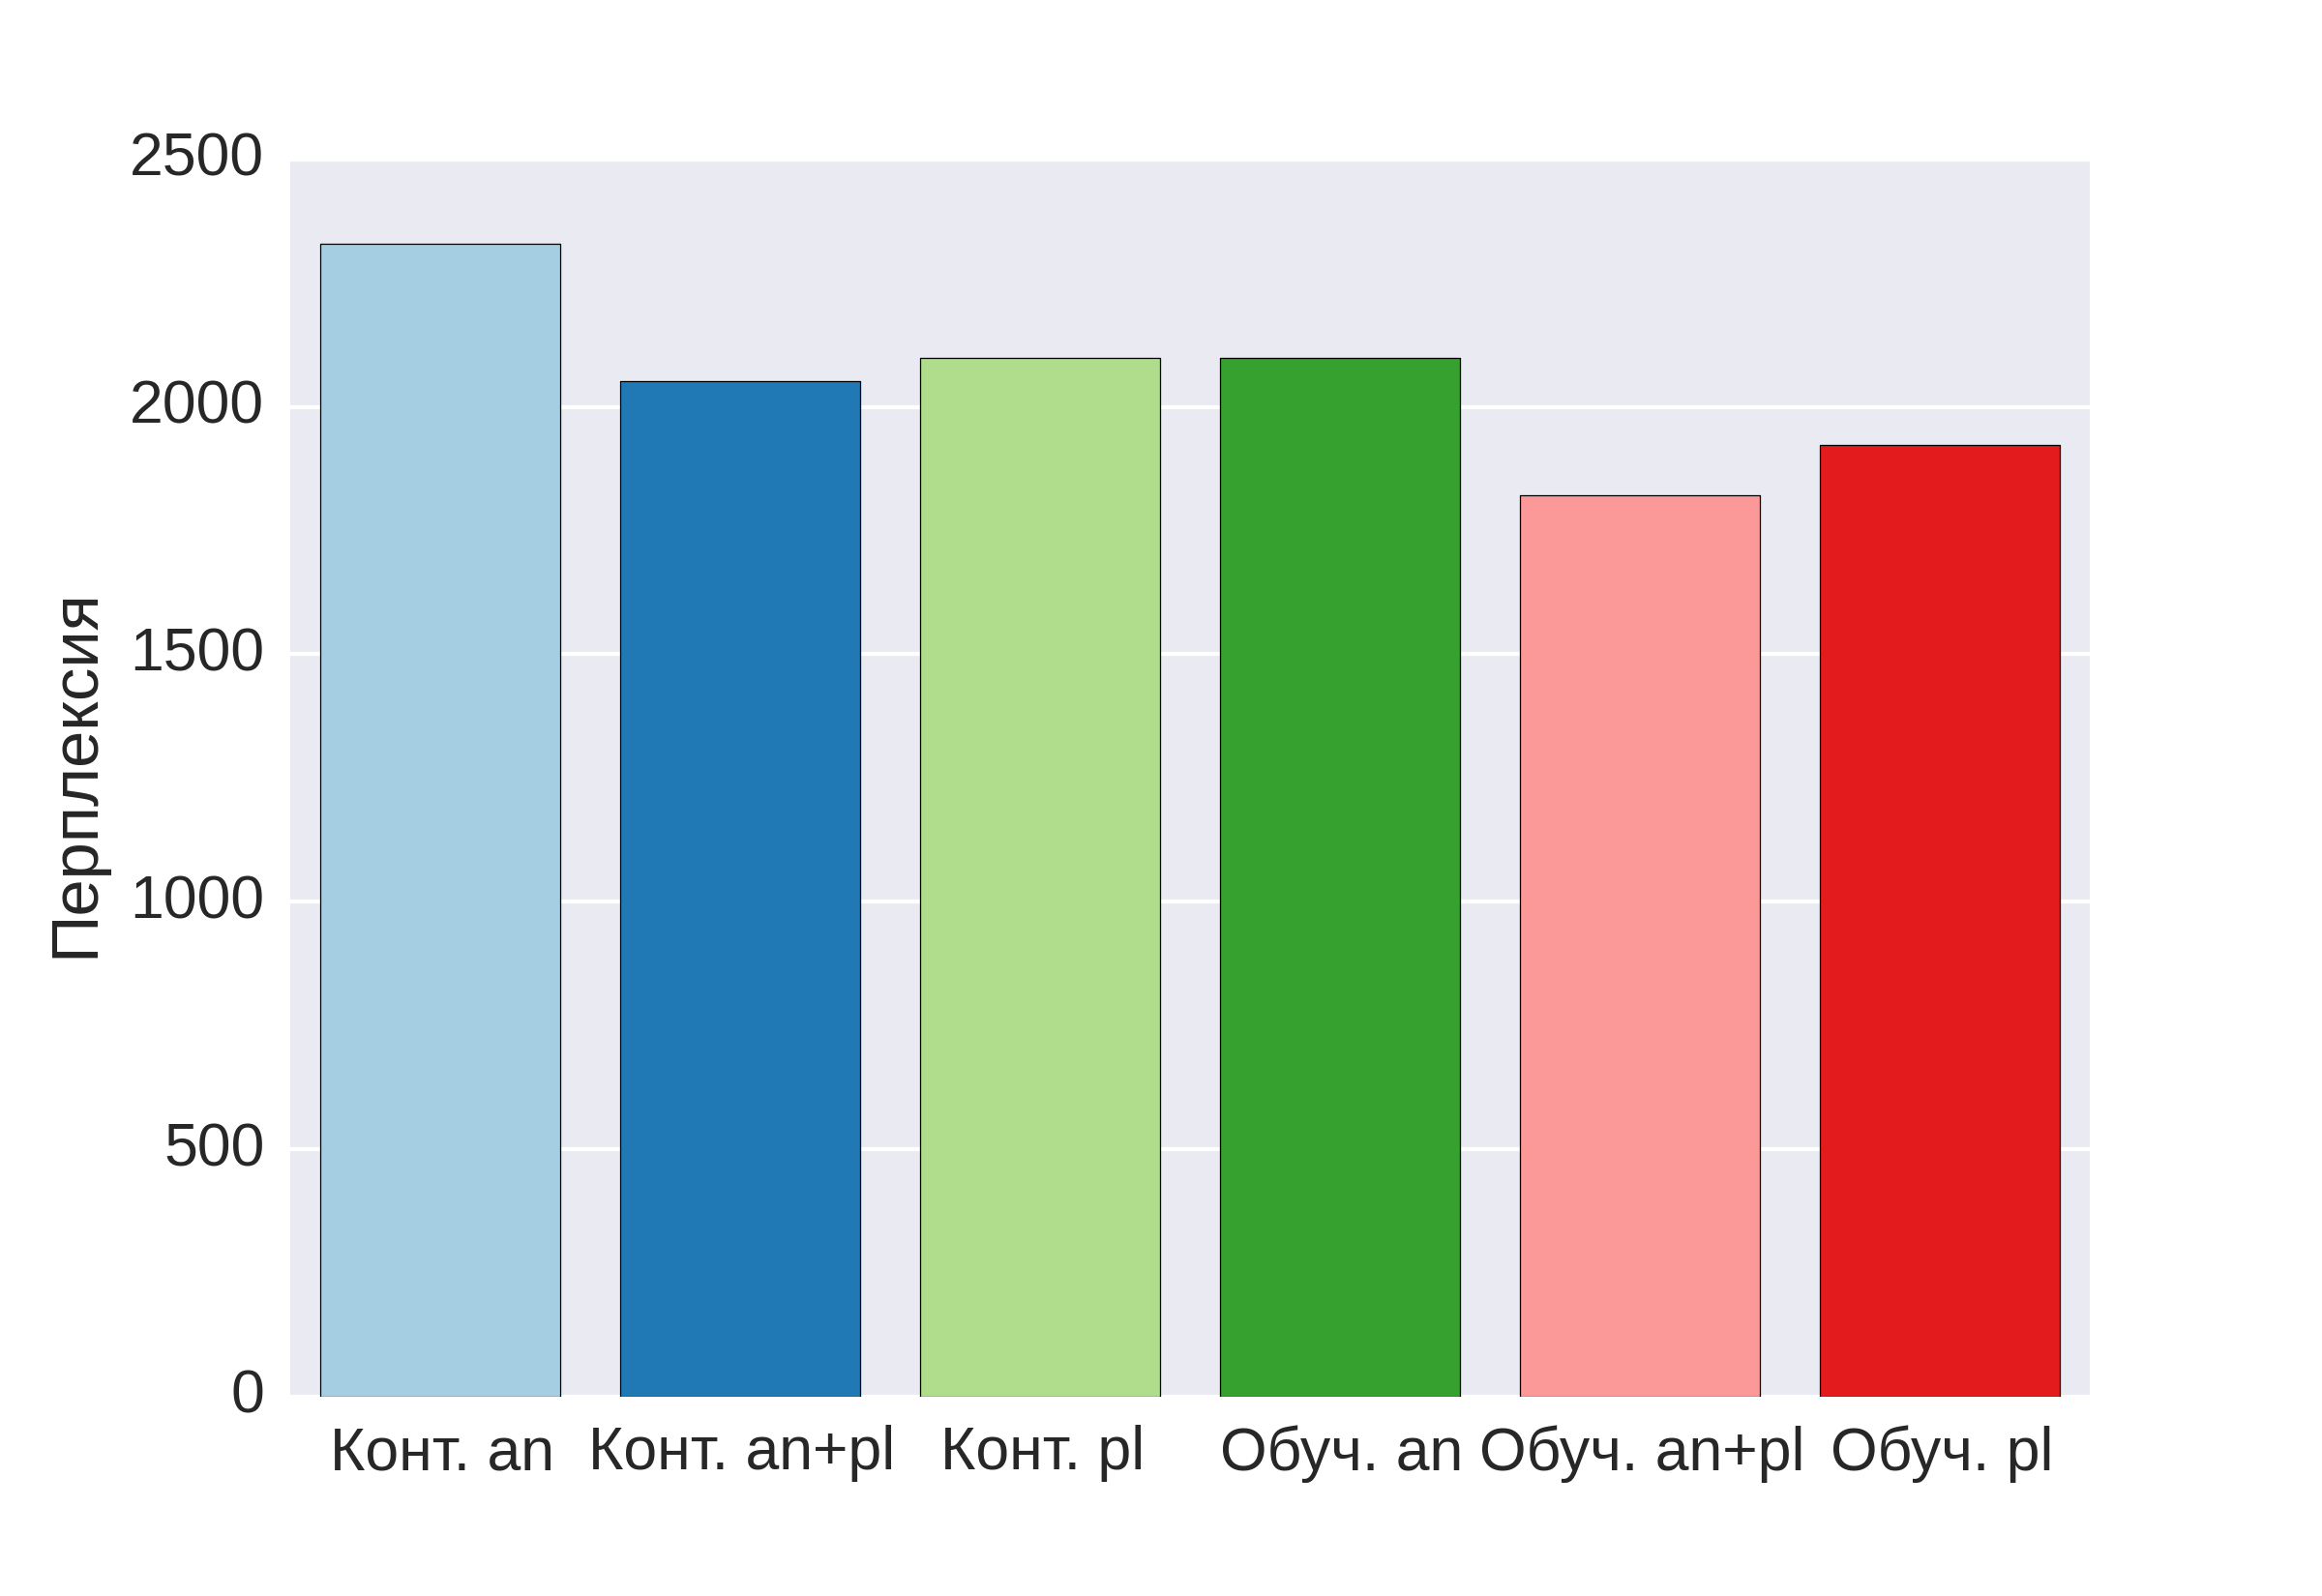
\includegraphics[scale=0.43]{img/anpl/5}
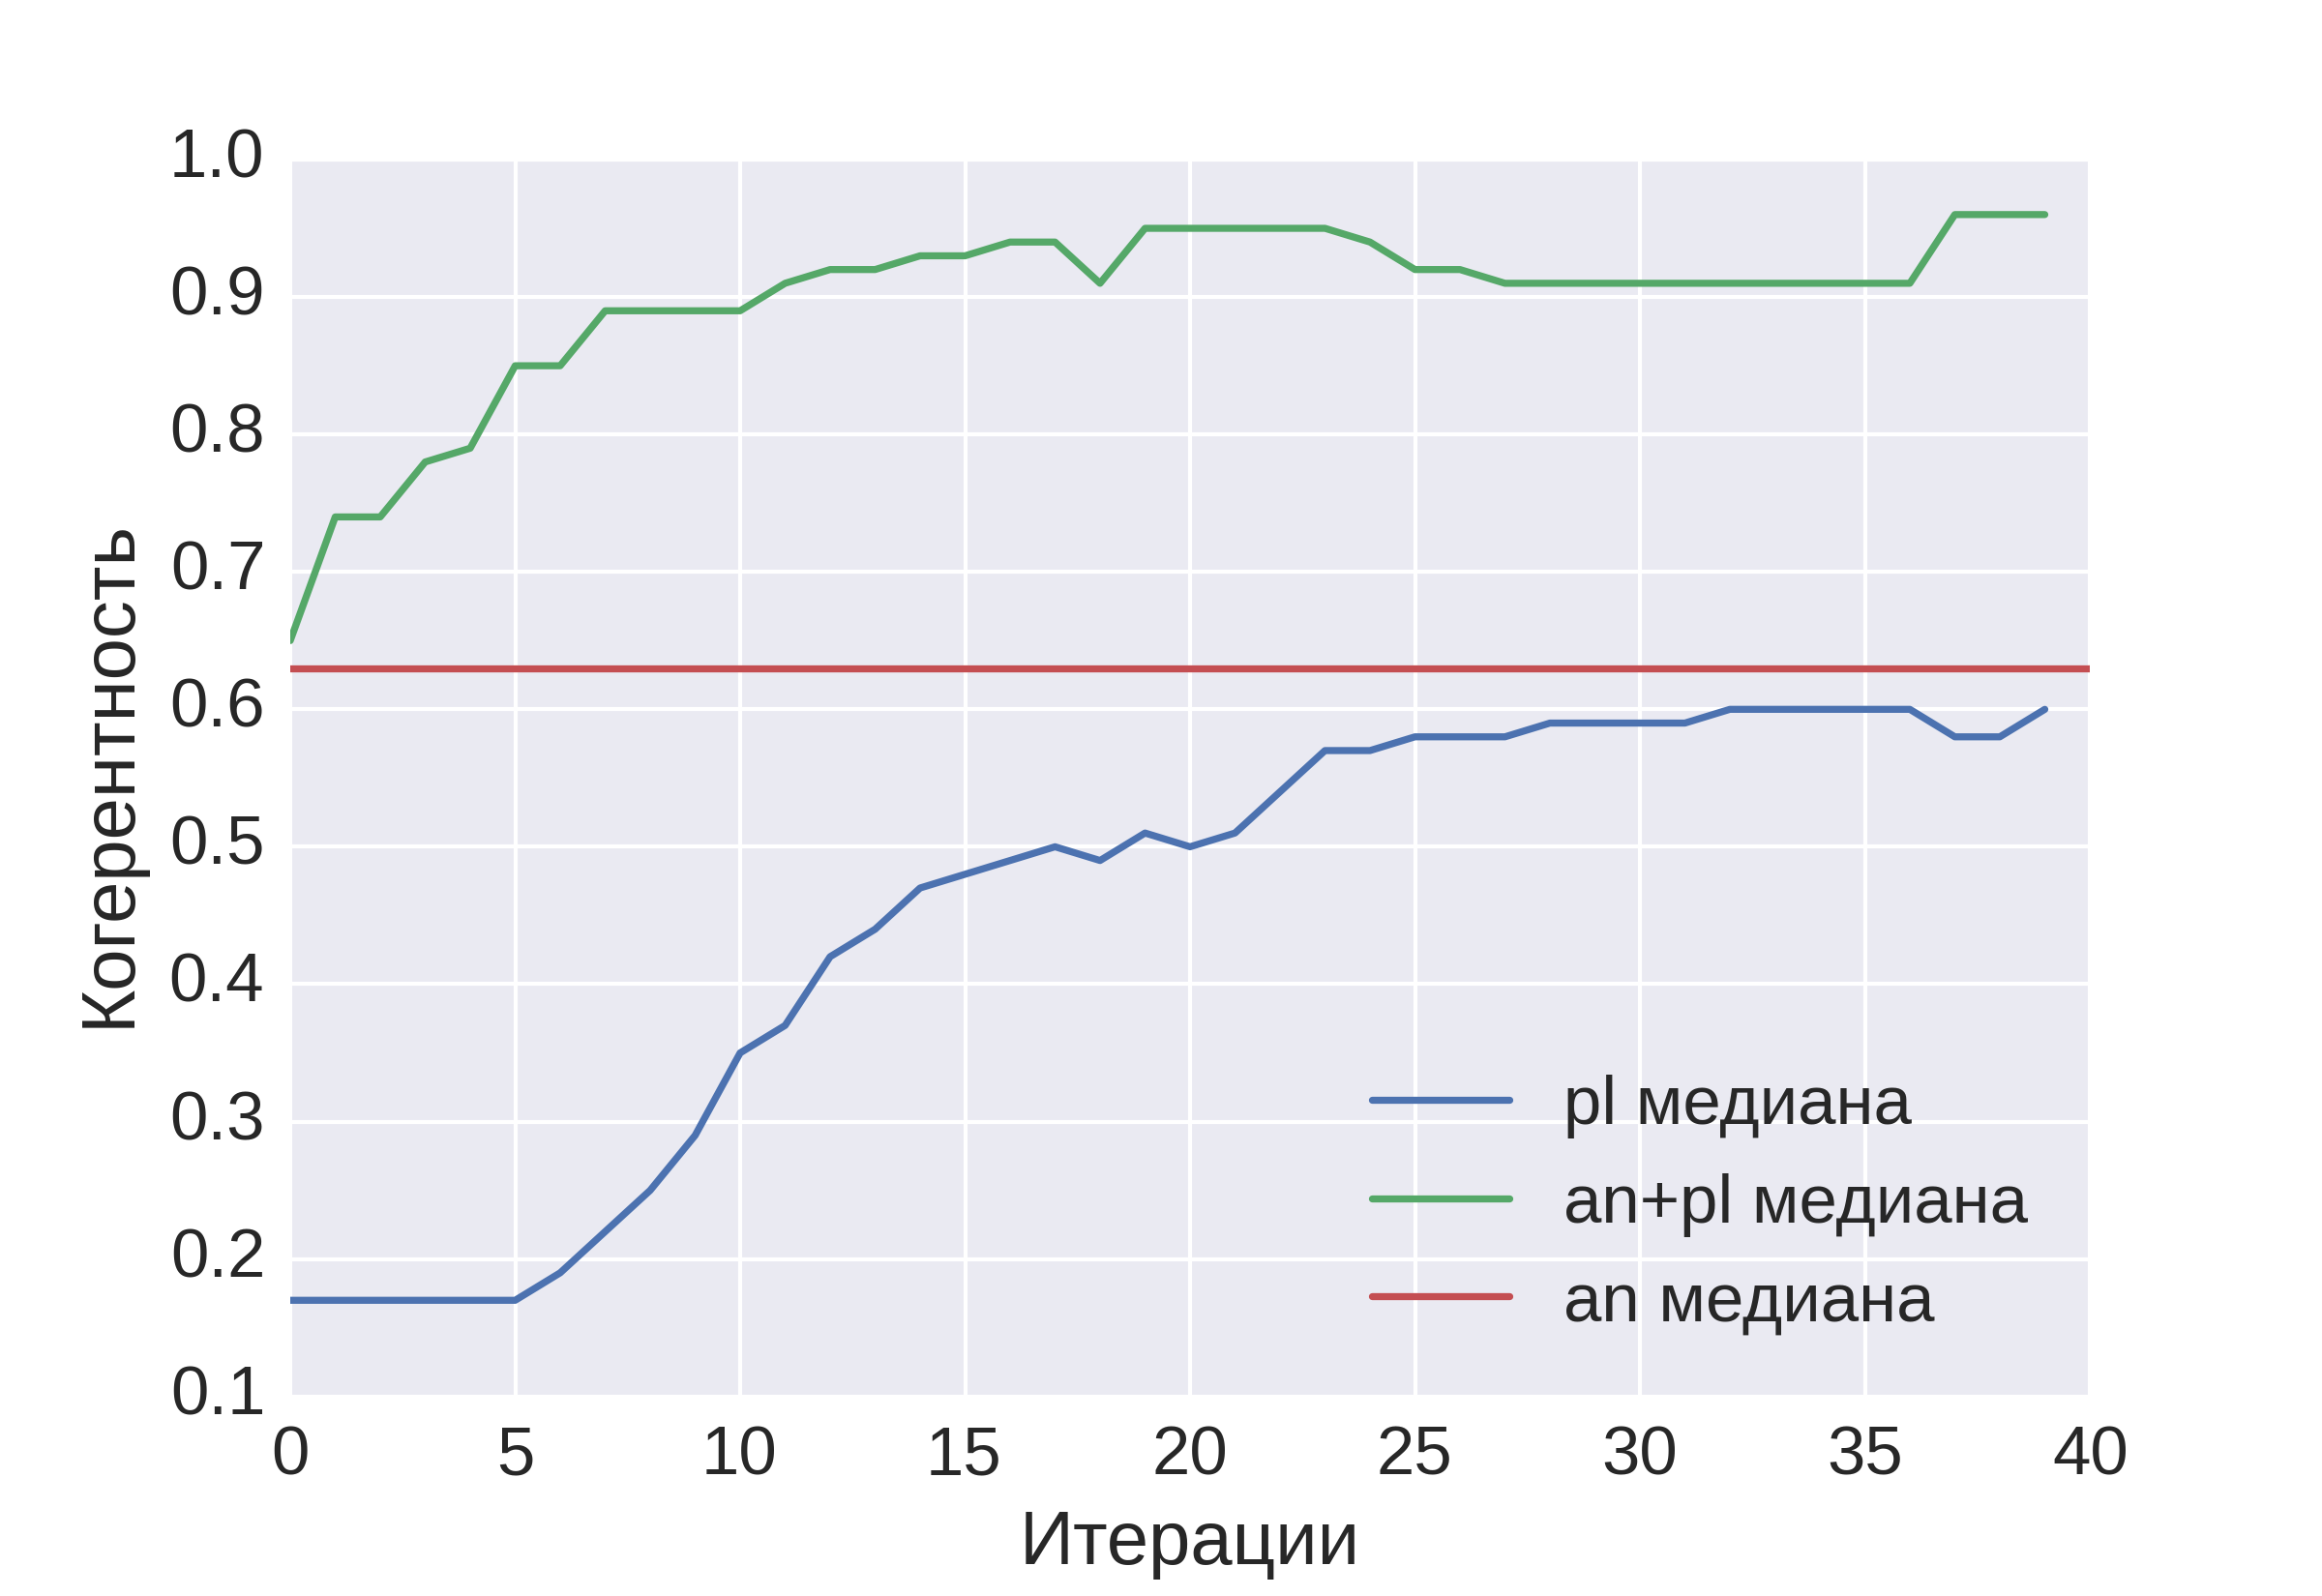
\includegraphics[scale=0.43]{img/anpl/3}
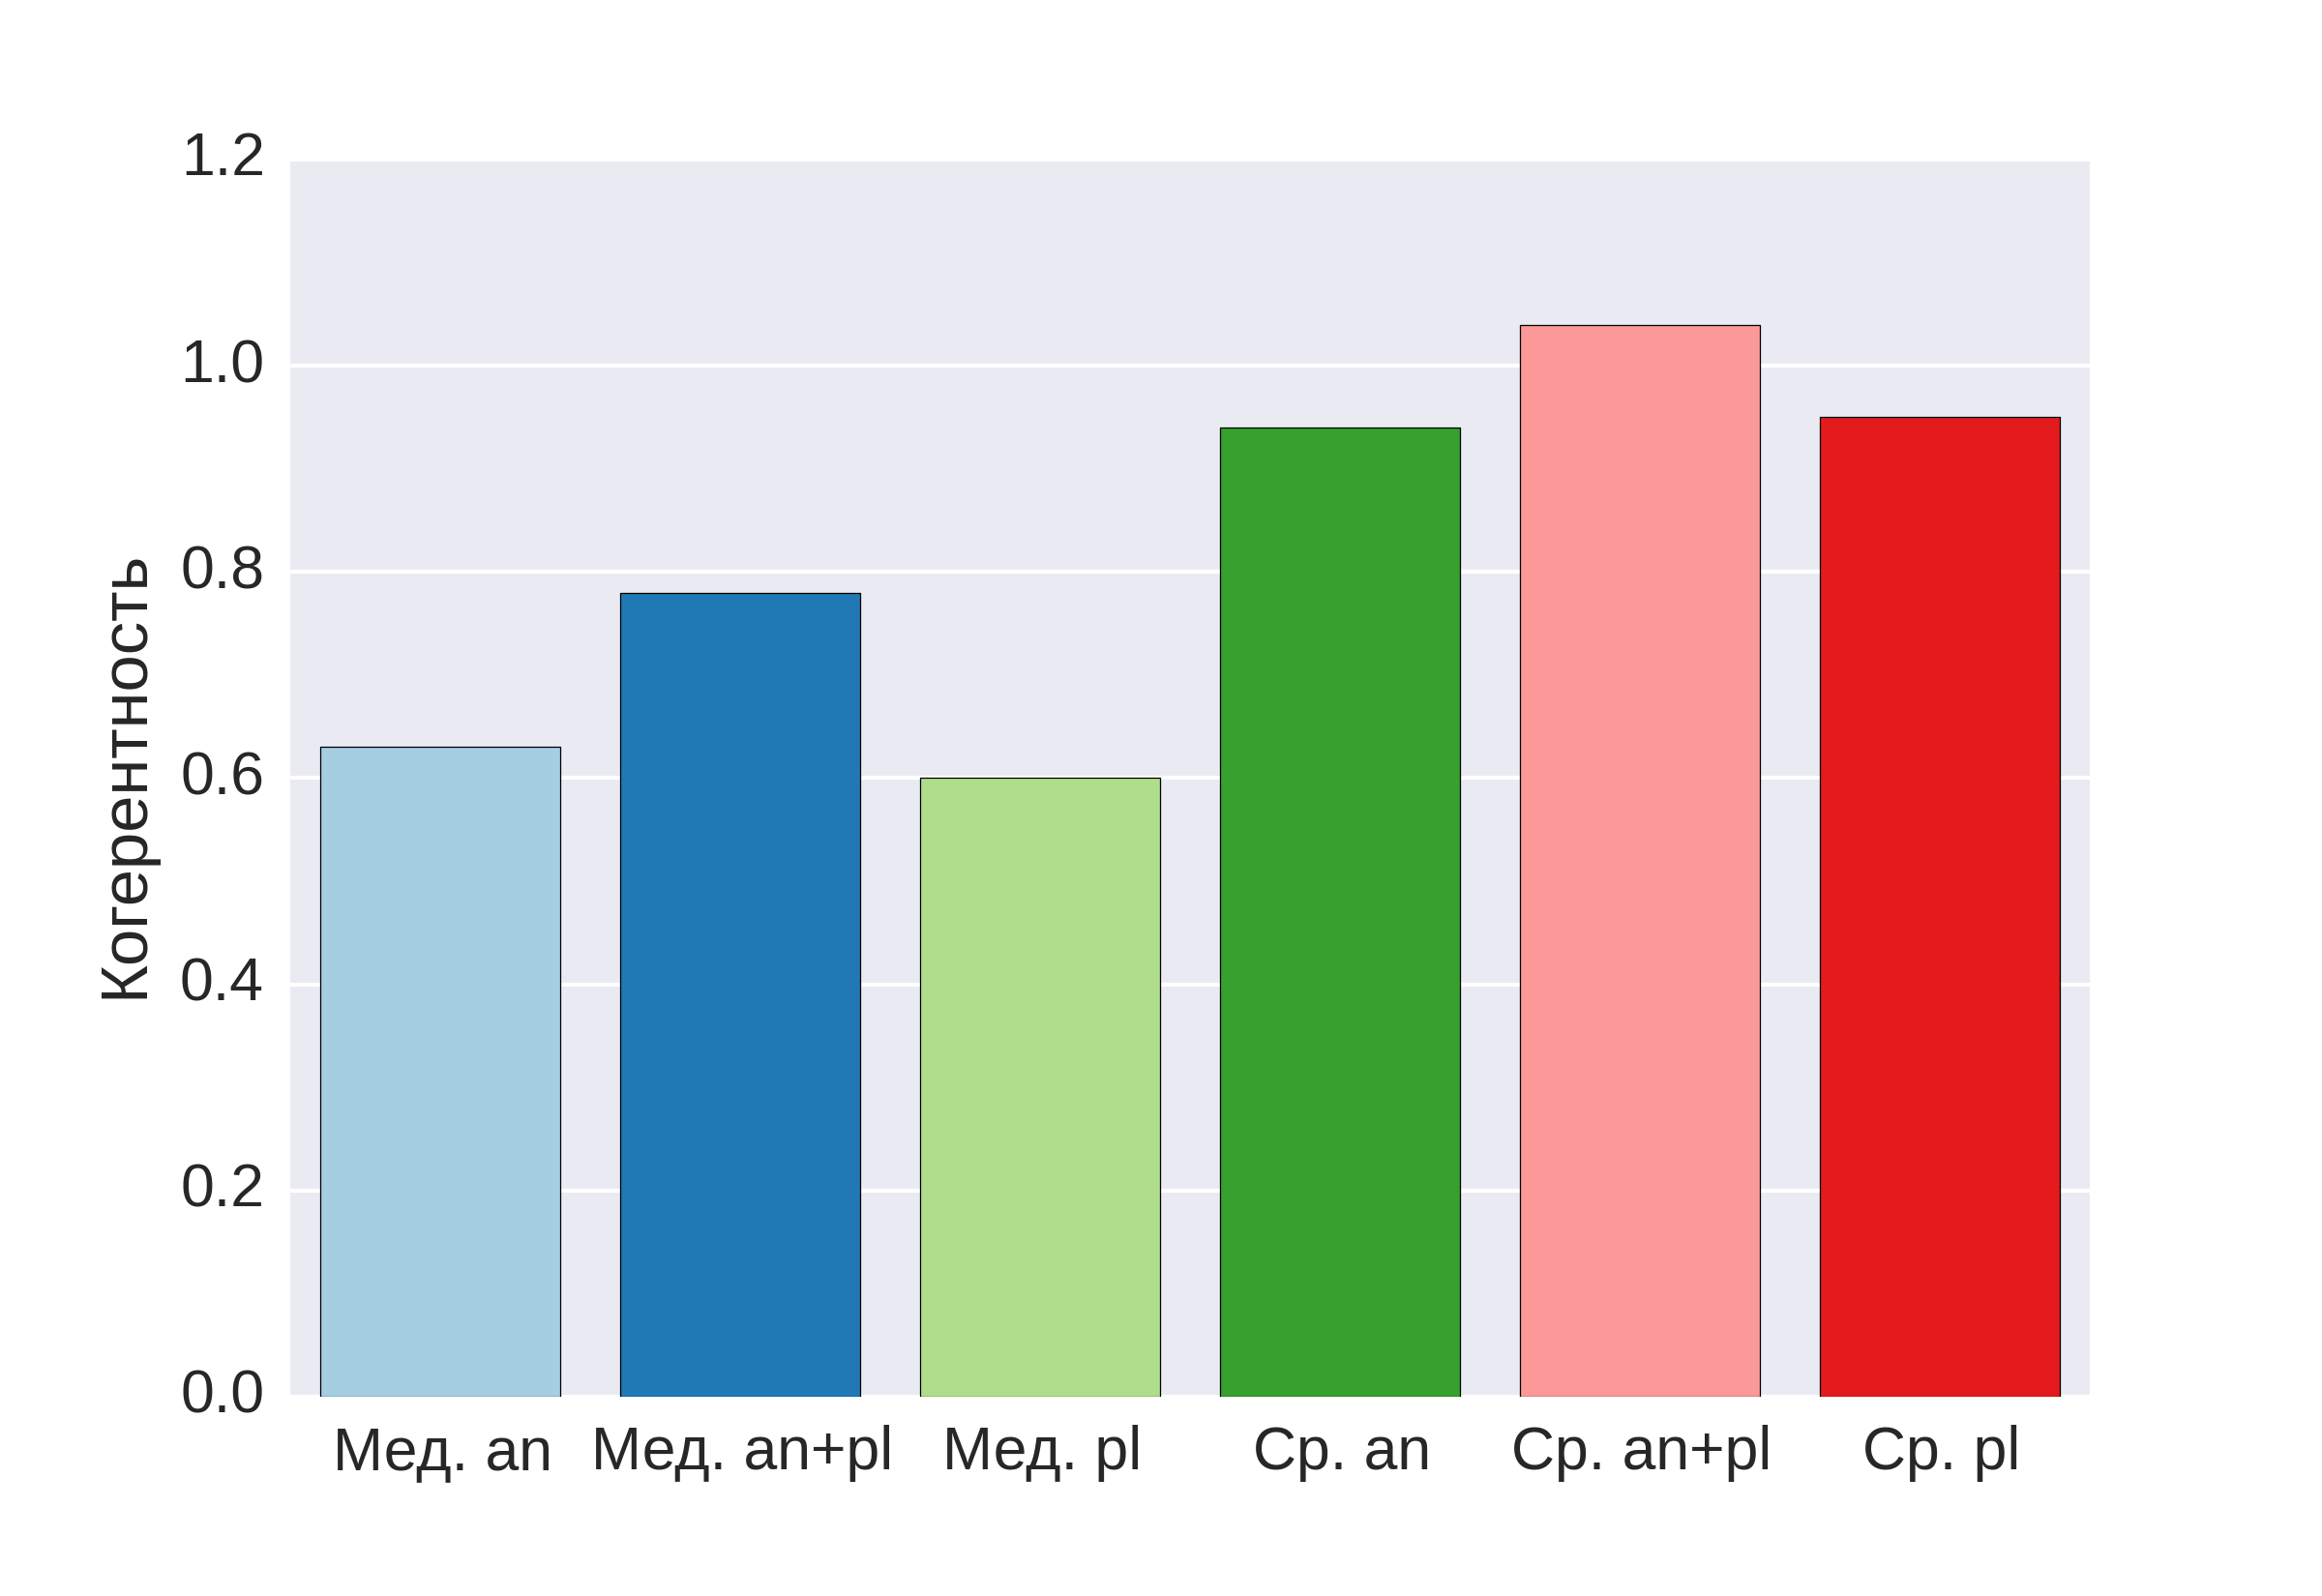
\includegraphics[scale=0.43]{img/anpl/6}\\
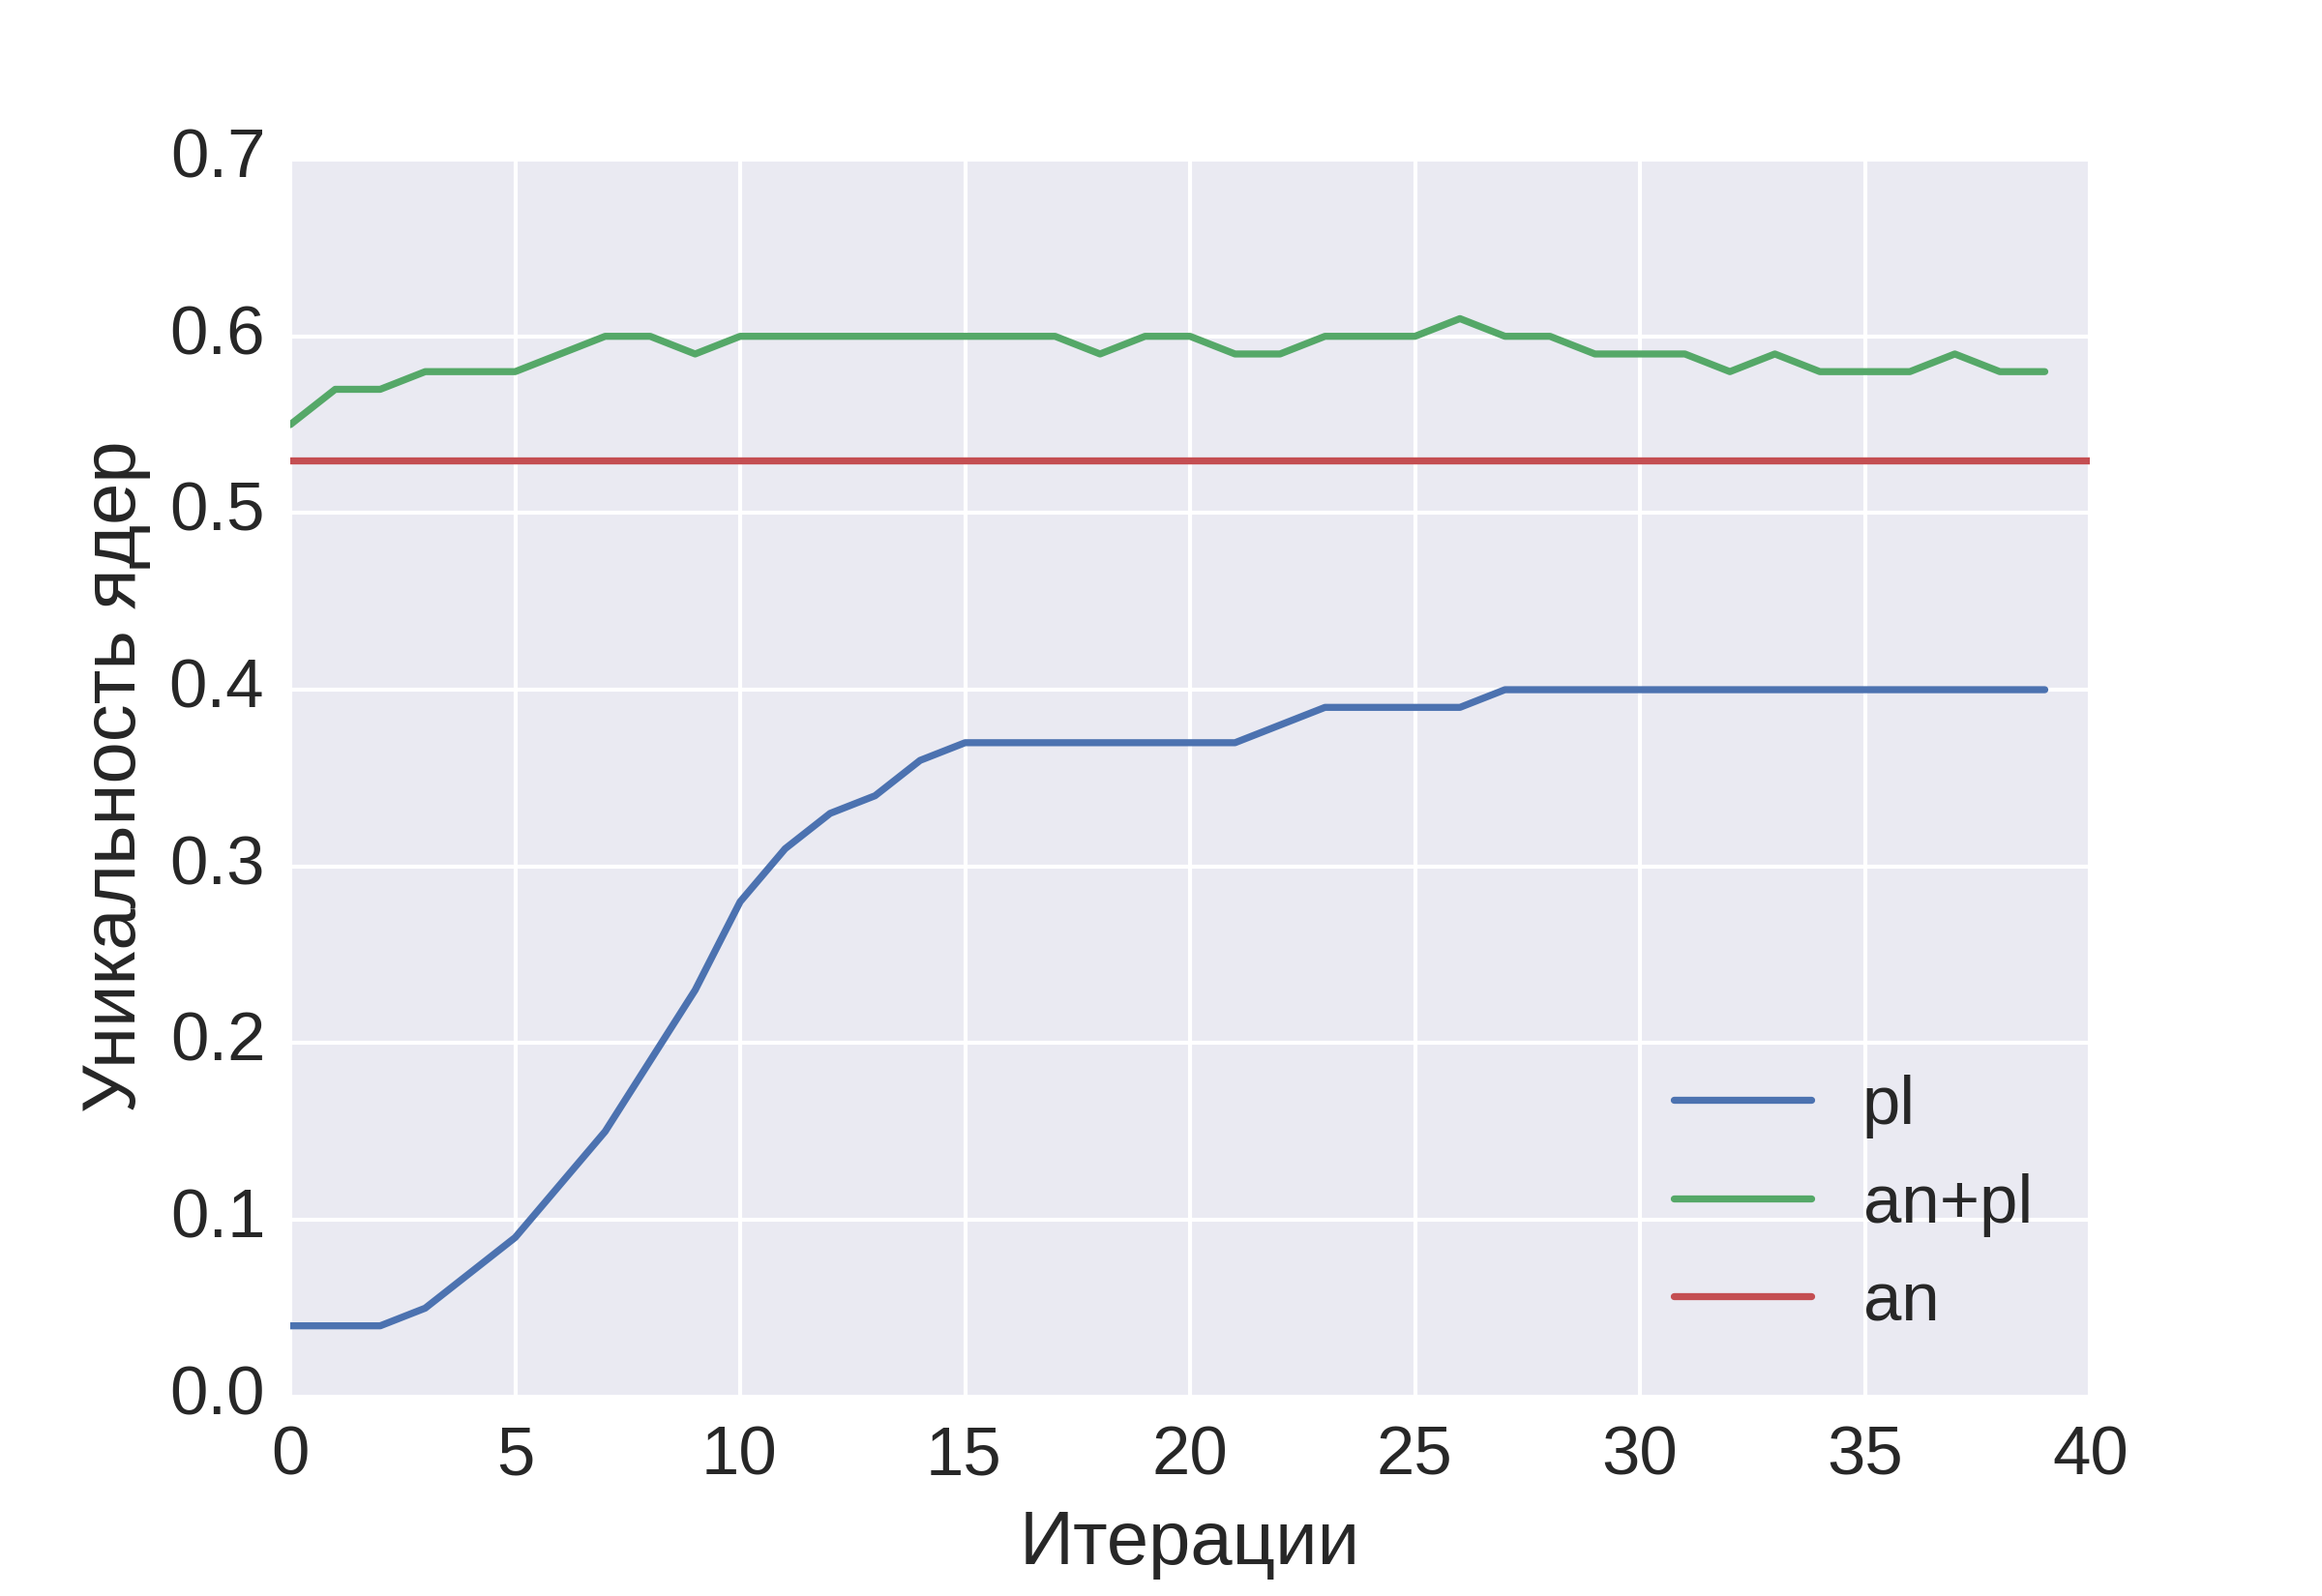
\includegraphics[scale=0.43]{img/anpl/4}
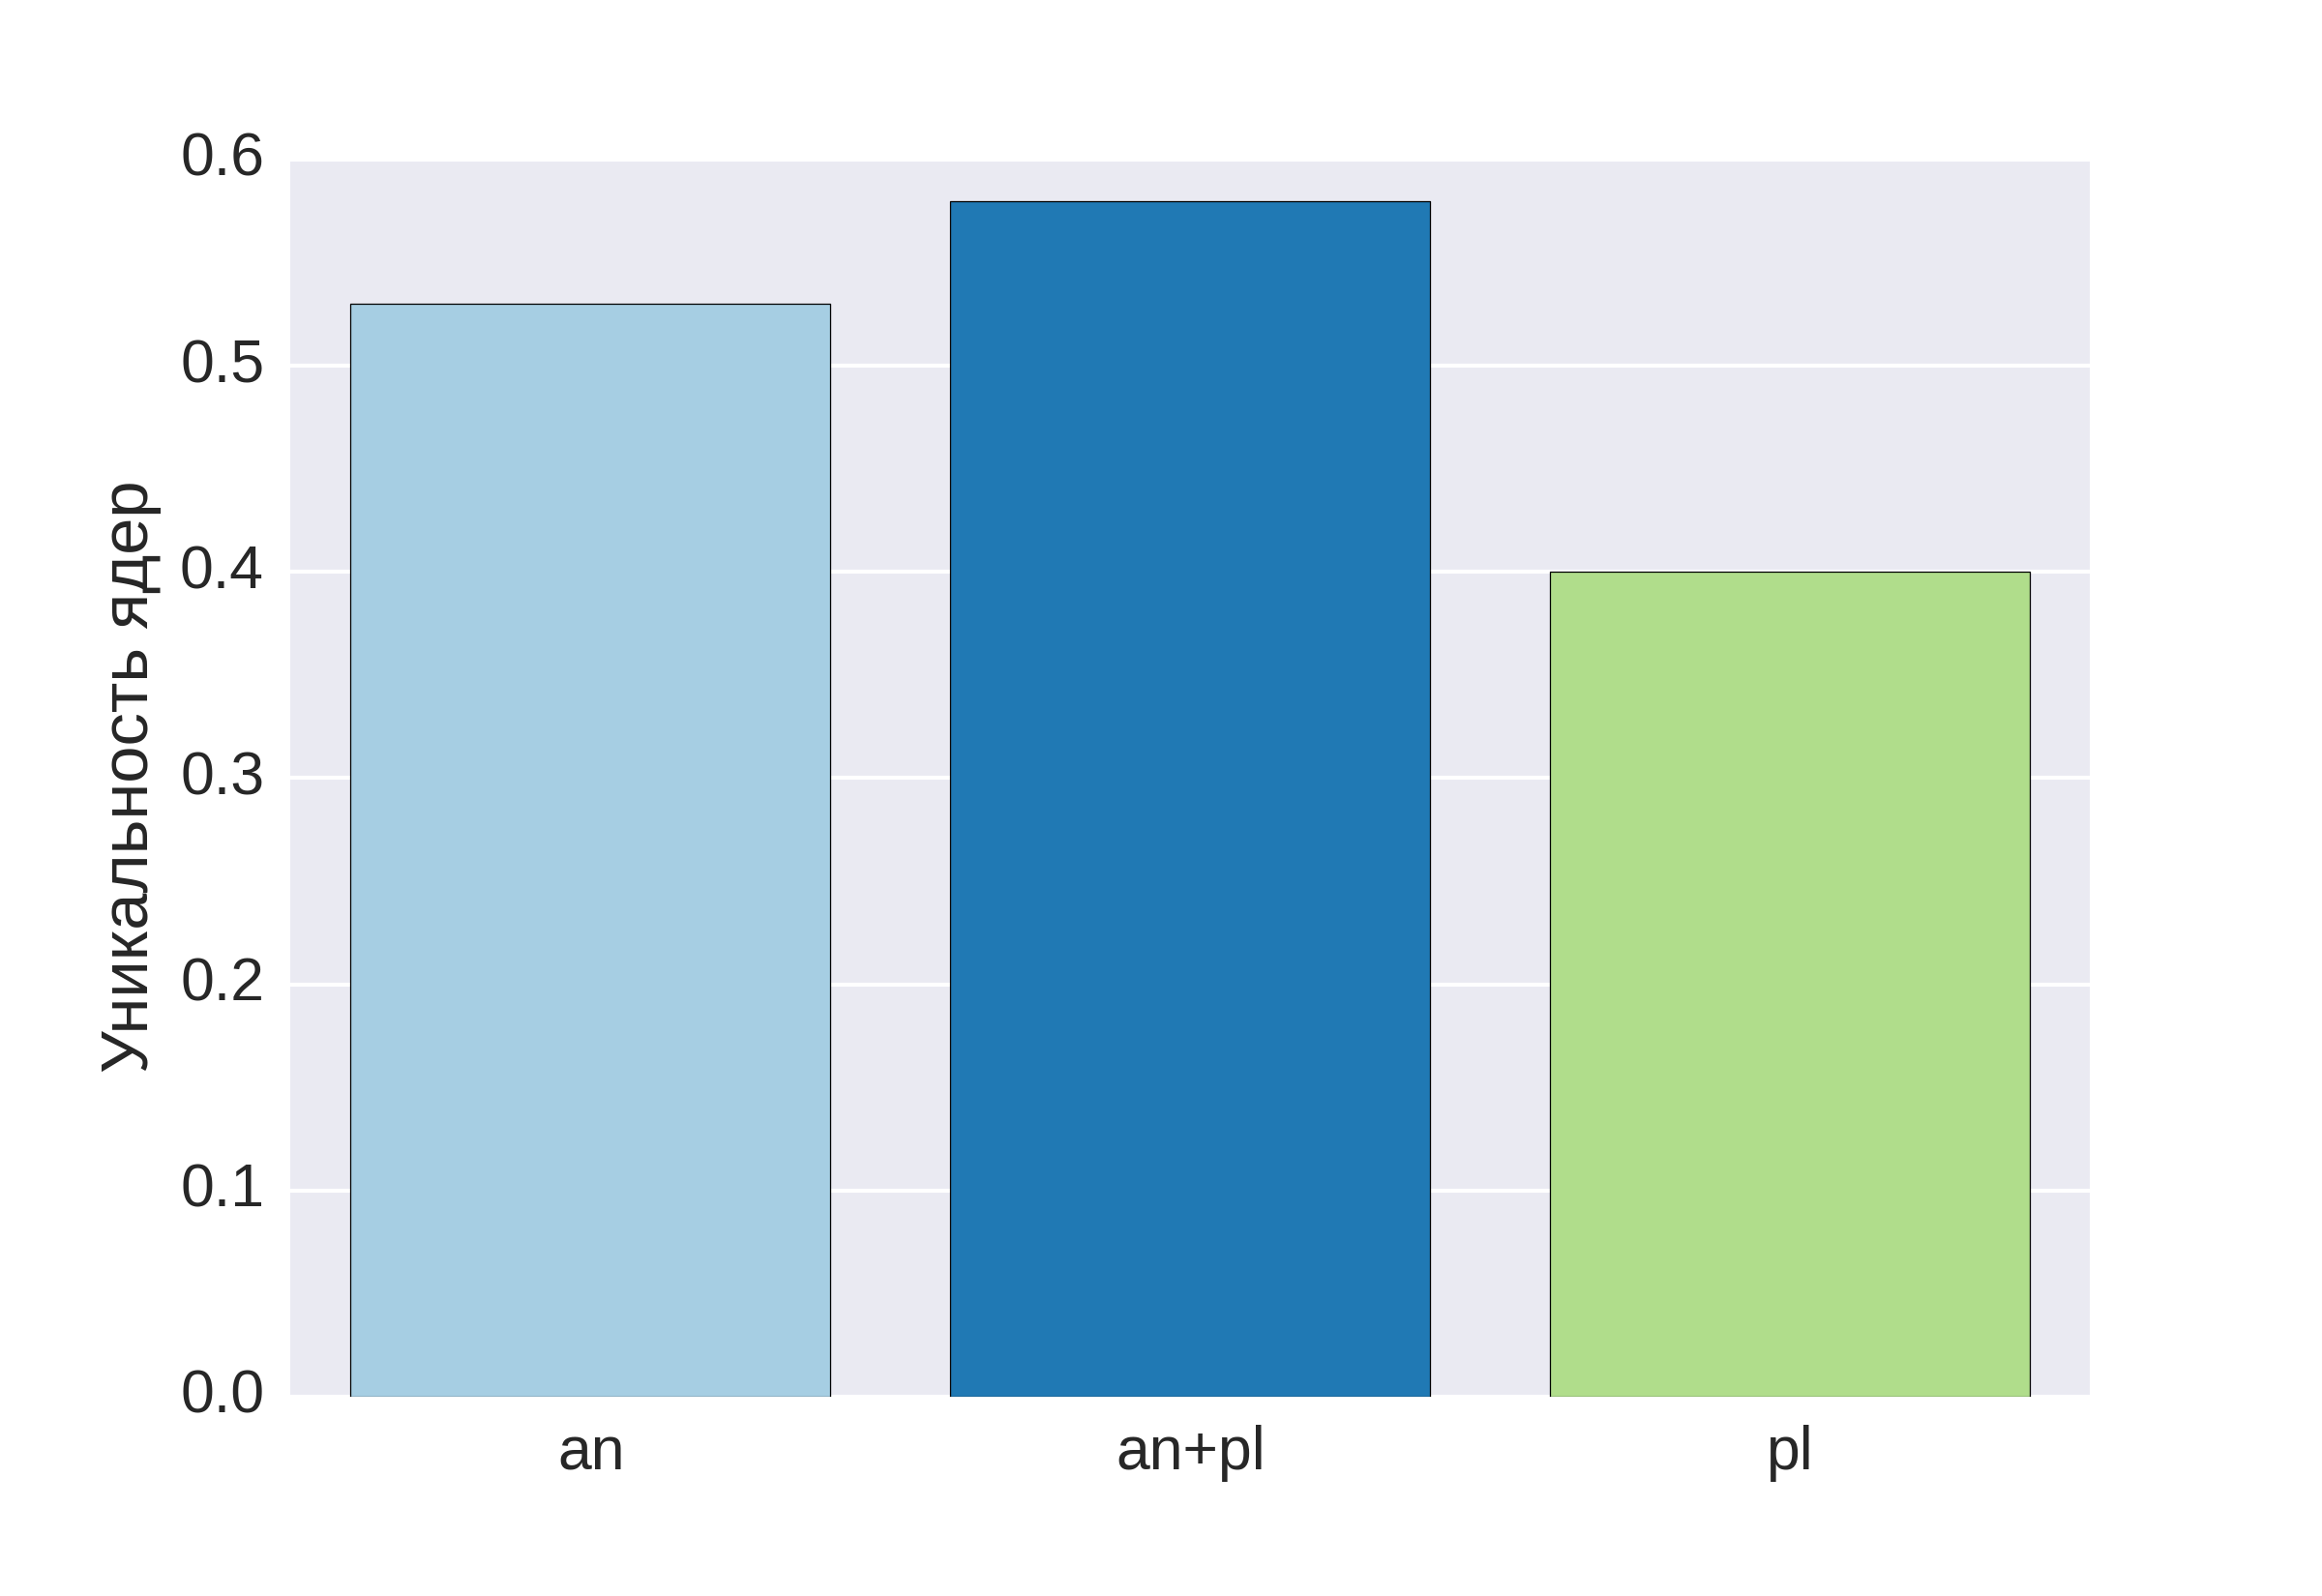
\includegraphics[scale=0.43]{img/anpl/7}

Рис. 10: Результаты экспериментов PLSA, Anchor Words, Комбинация PLSA и Anchor Words.



\subsection{Поиск кандидатов в Anchor Words}
\subsubsection*{Лингвистические требования к тематически окрашенным терминам}
В реализации предложенной авторами на термины, которые могли стать якорными накладывались частотные ограничения для устранения шумов.

Но термины помимо своих частотных характеристик обладают также и лингвистическими характеристиками -- морфологическими, грамматическими, и  др.

Было выдвинуто предположение, что якорными словами могли стать те термины, которые прошли частотный отбор и являются существительными.

Эксперименты показали что при добавлении морфологических ограничений перплексия уменьшается, средняя интерпретируемость возрастает,  но медиана интерпретируемости и уникальность ядер ведет себя нестабильно.
\subsubsection*{Эксперименты}


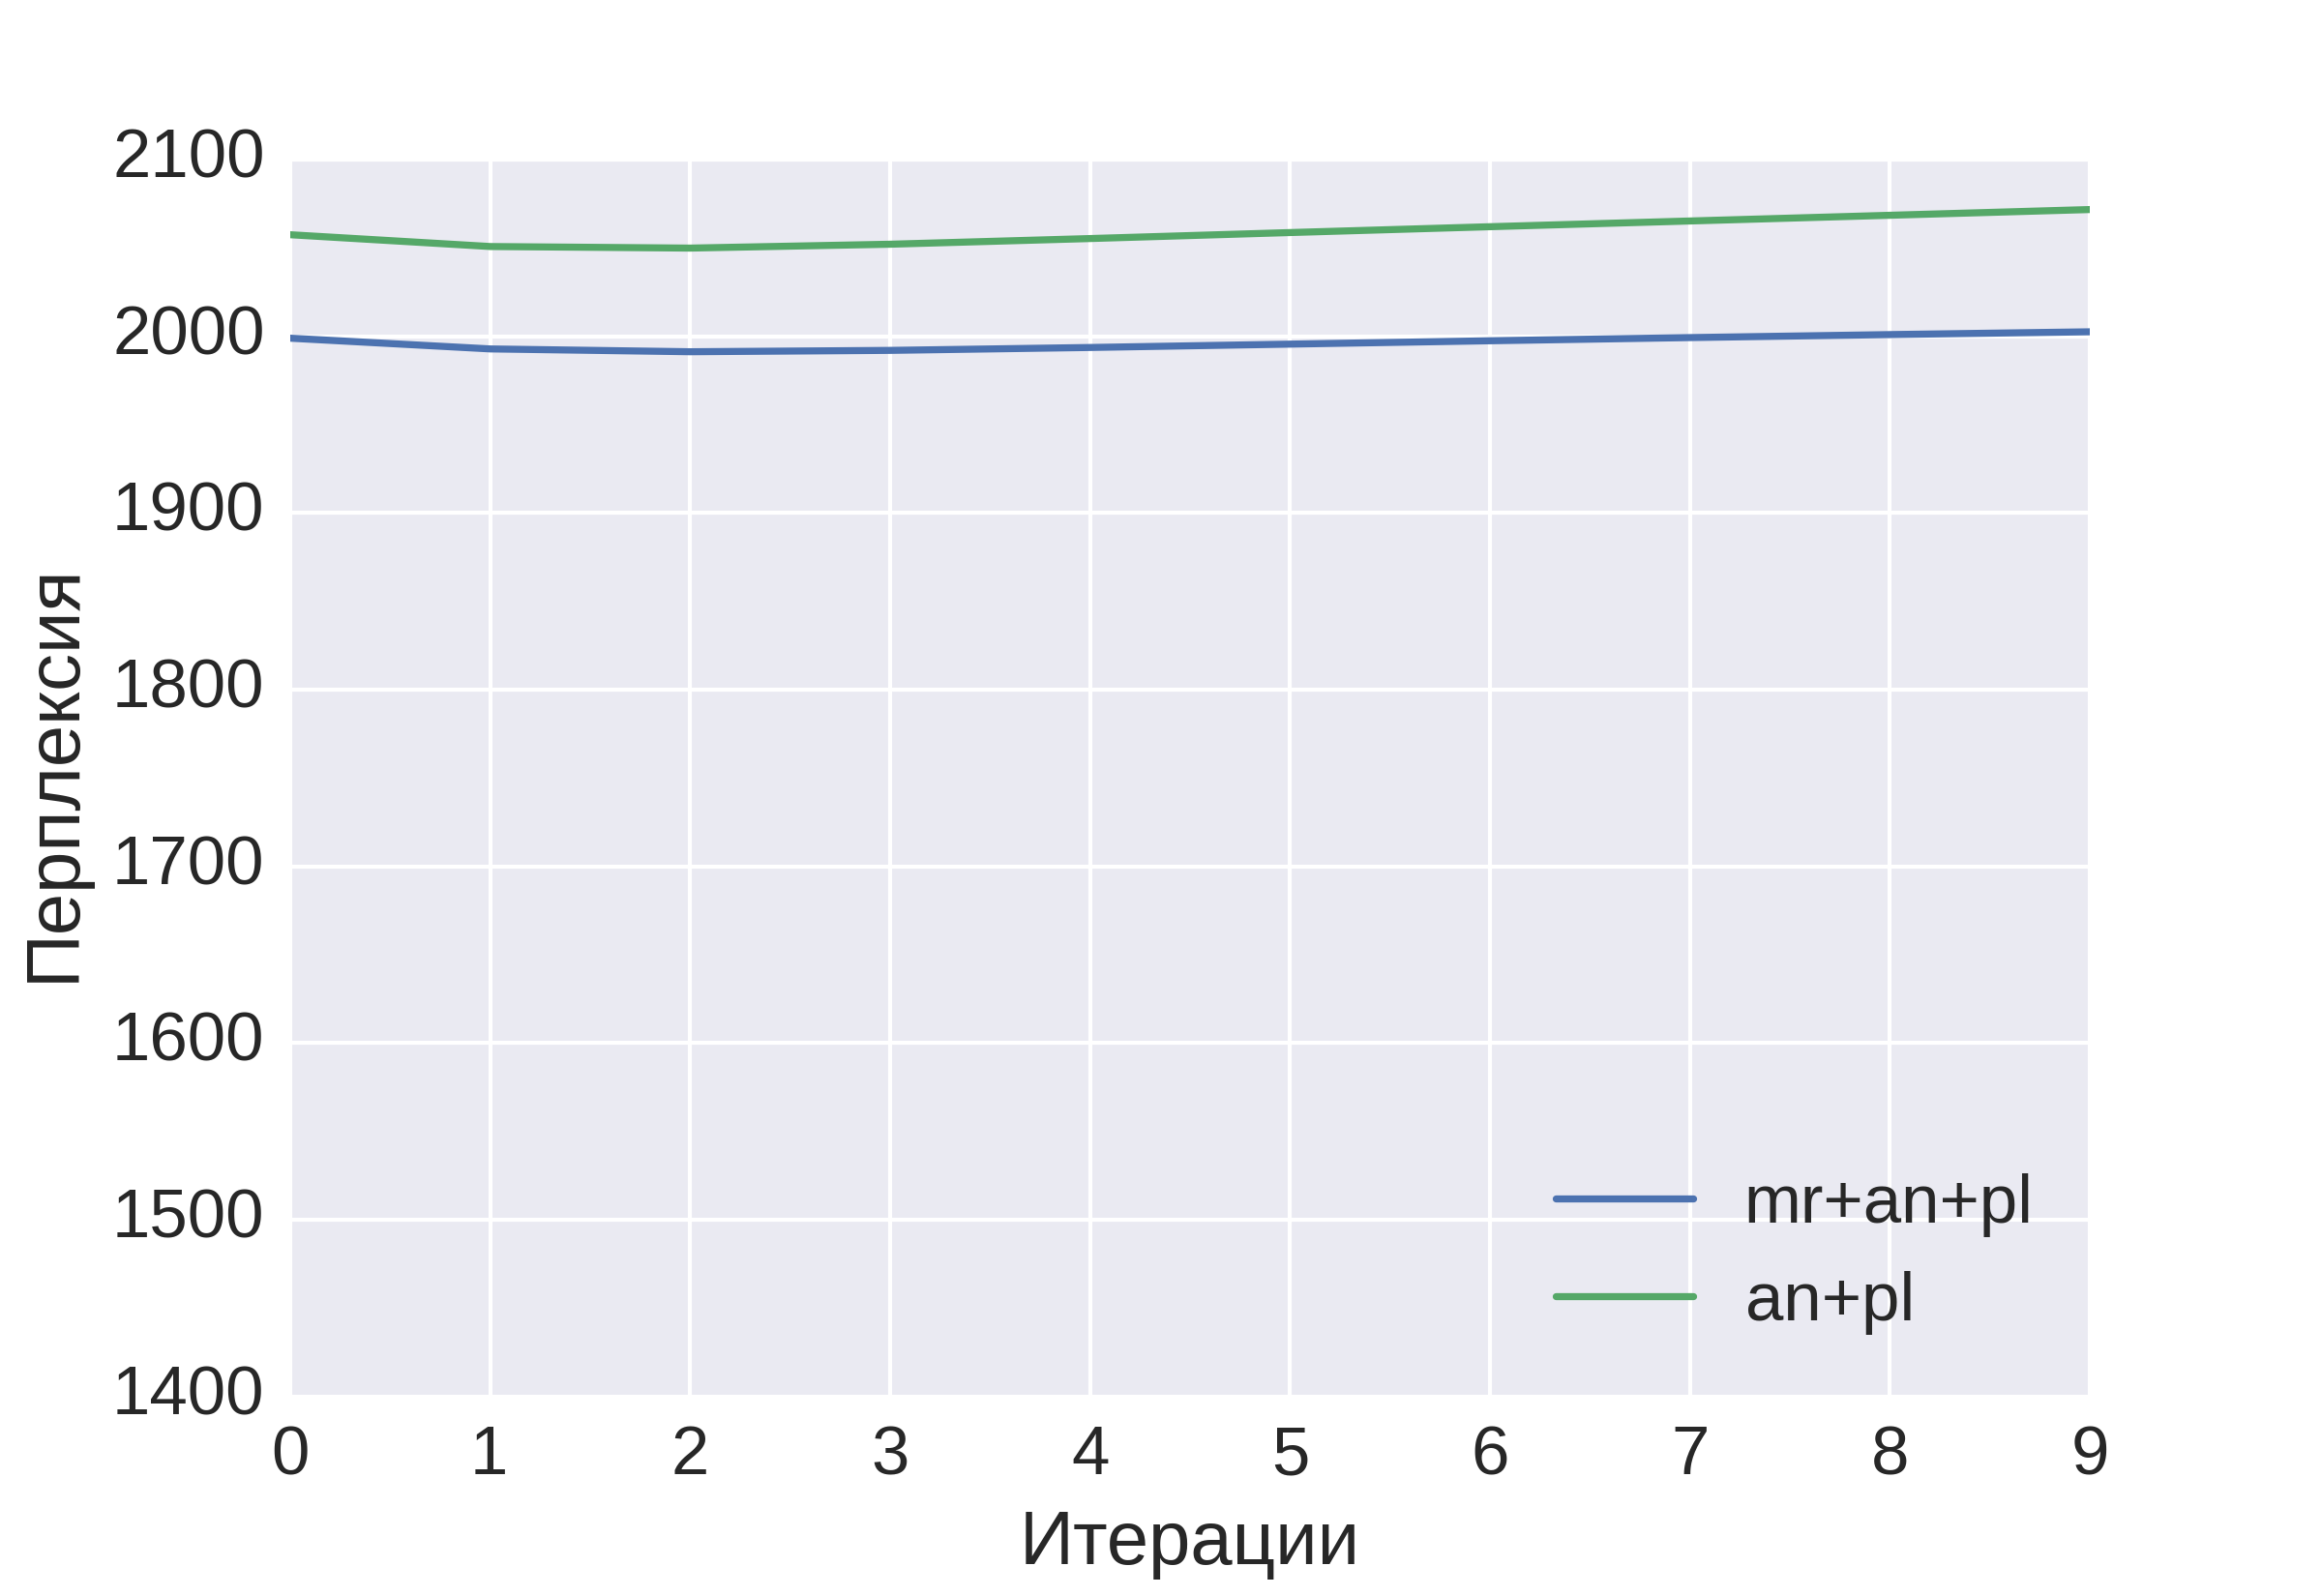
\includegraphics[scale=0.43]{img/no/1}
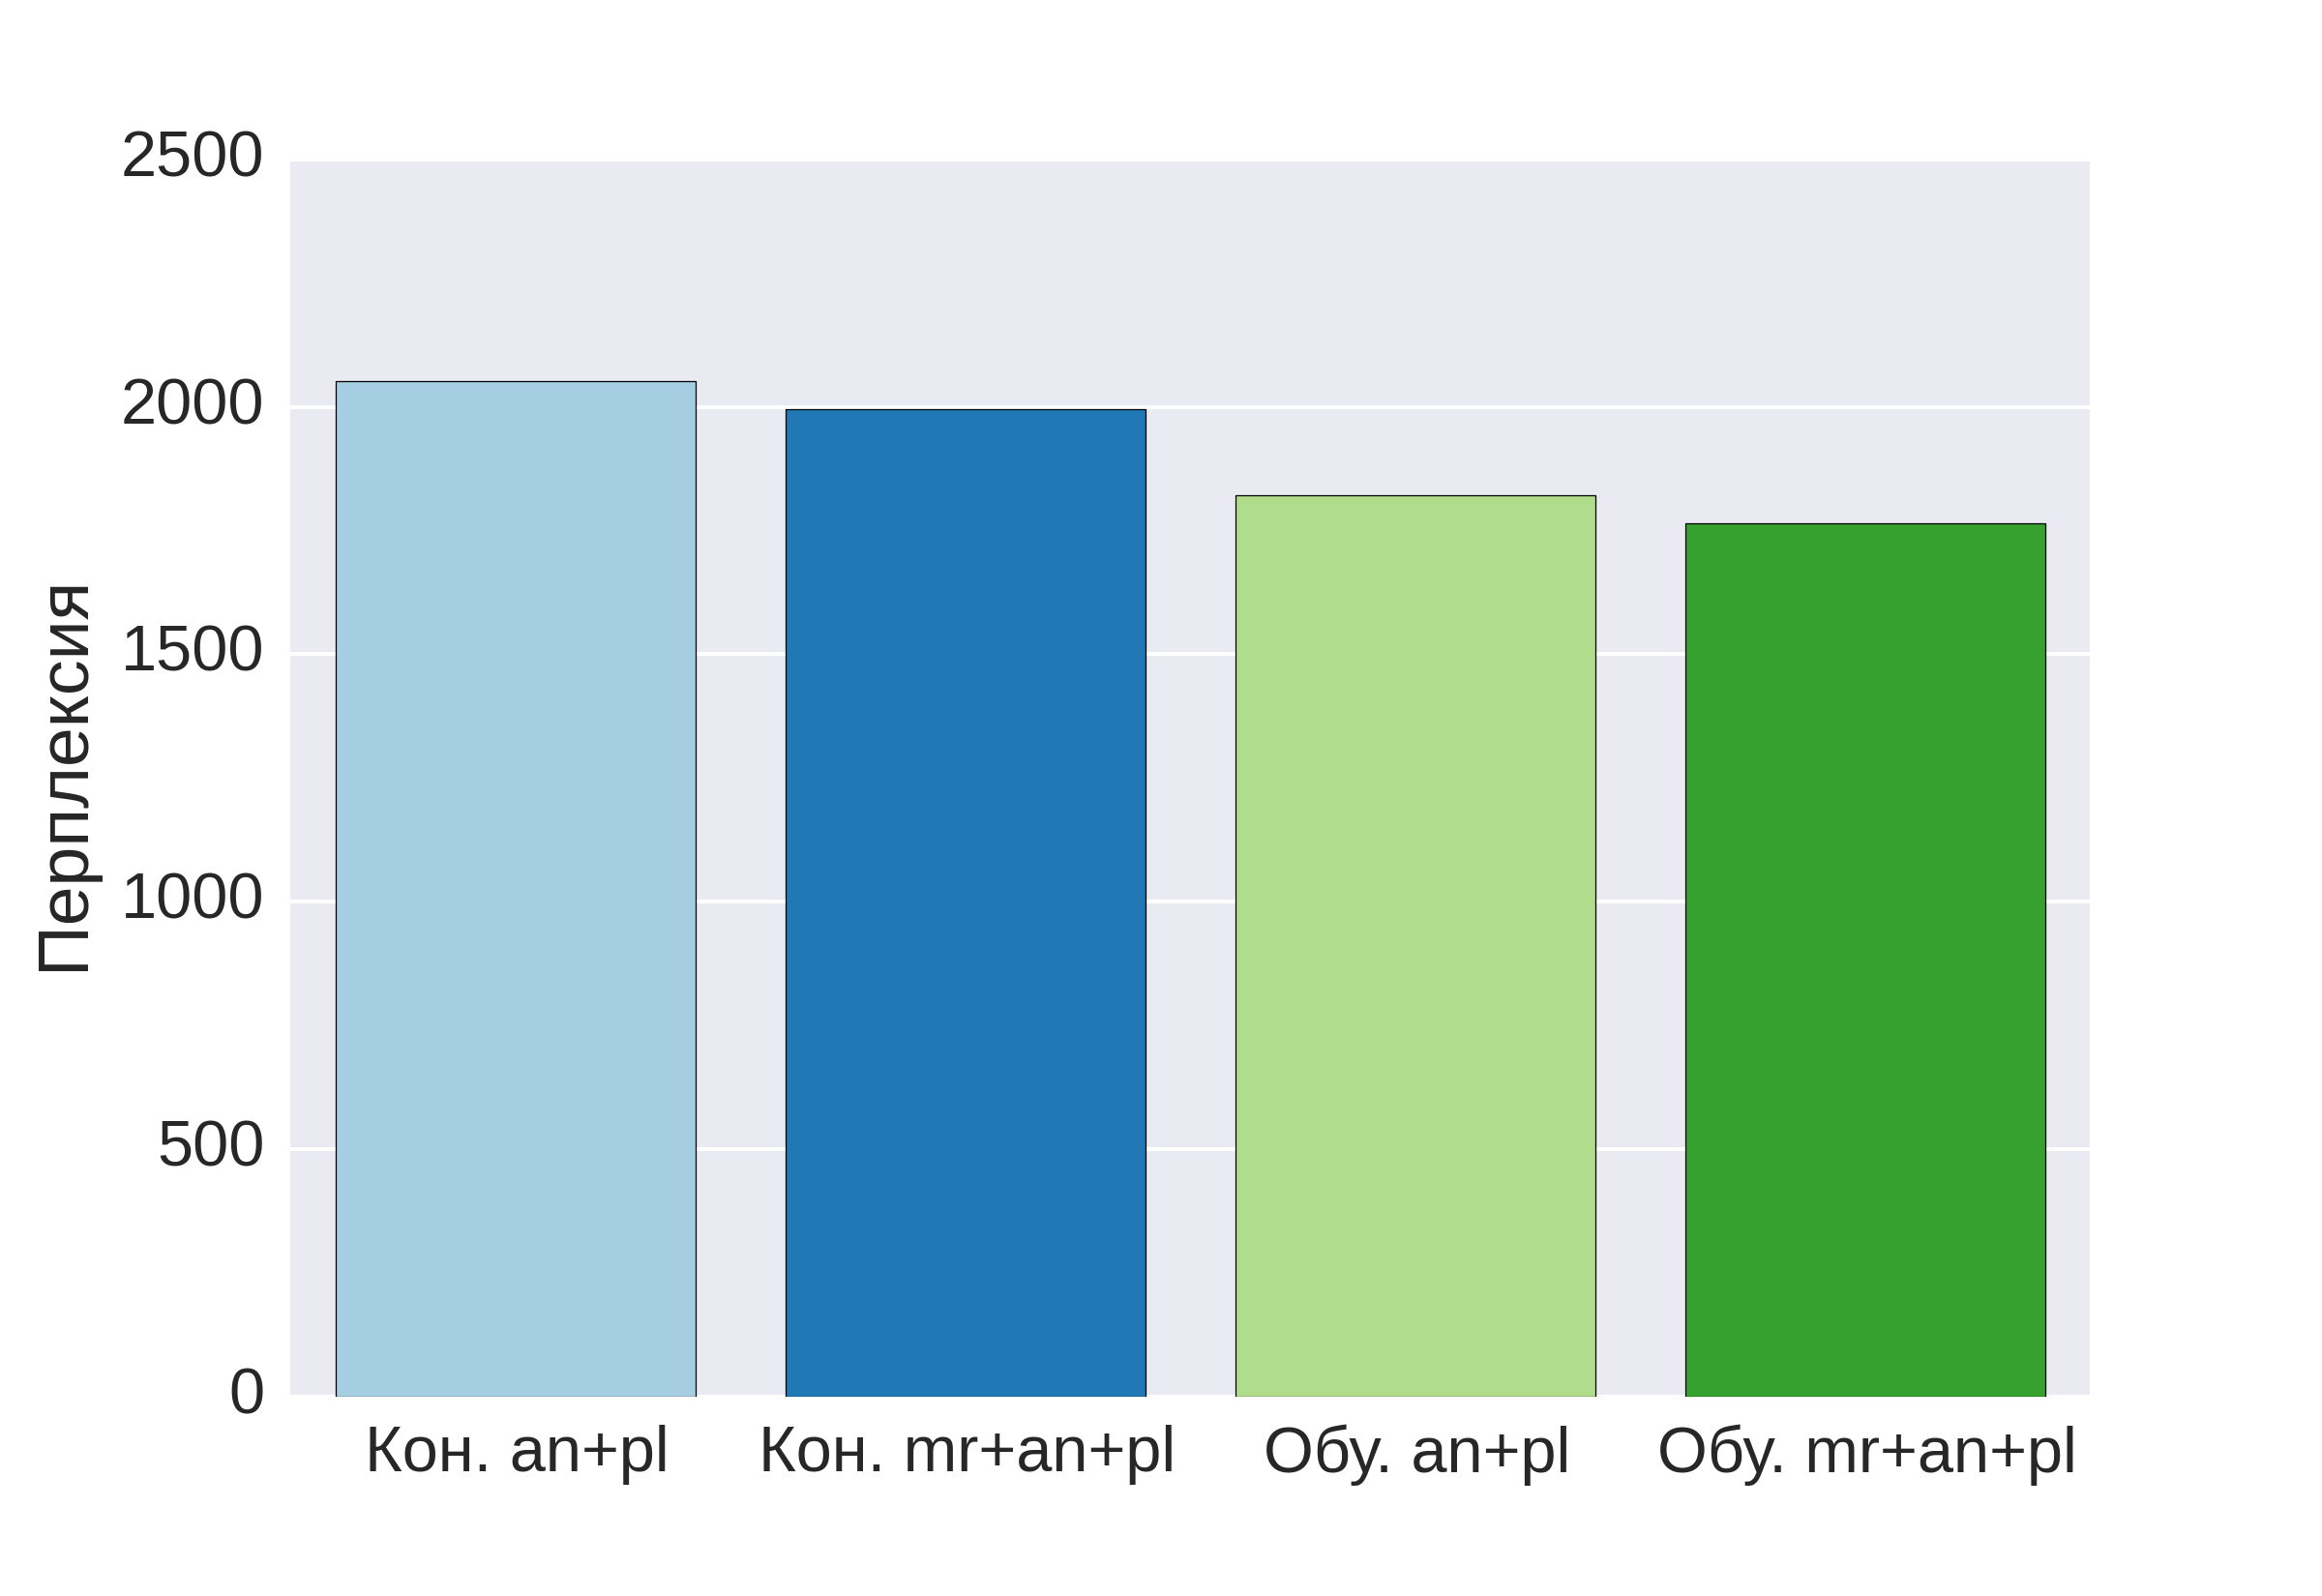
\includegraphics[scale=0.43]{img/no/5}\\
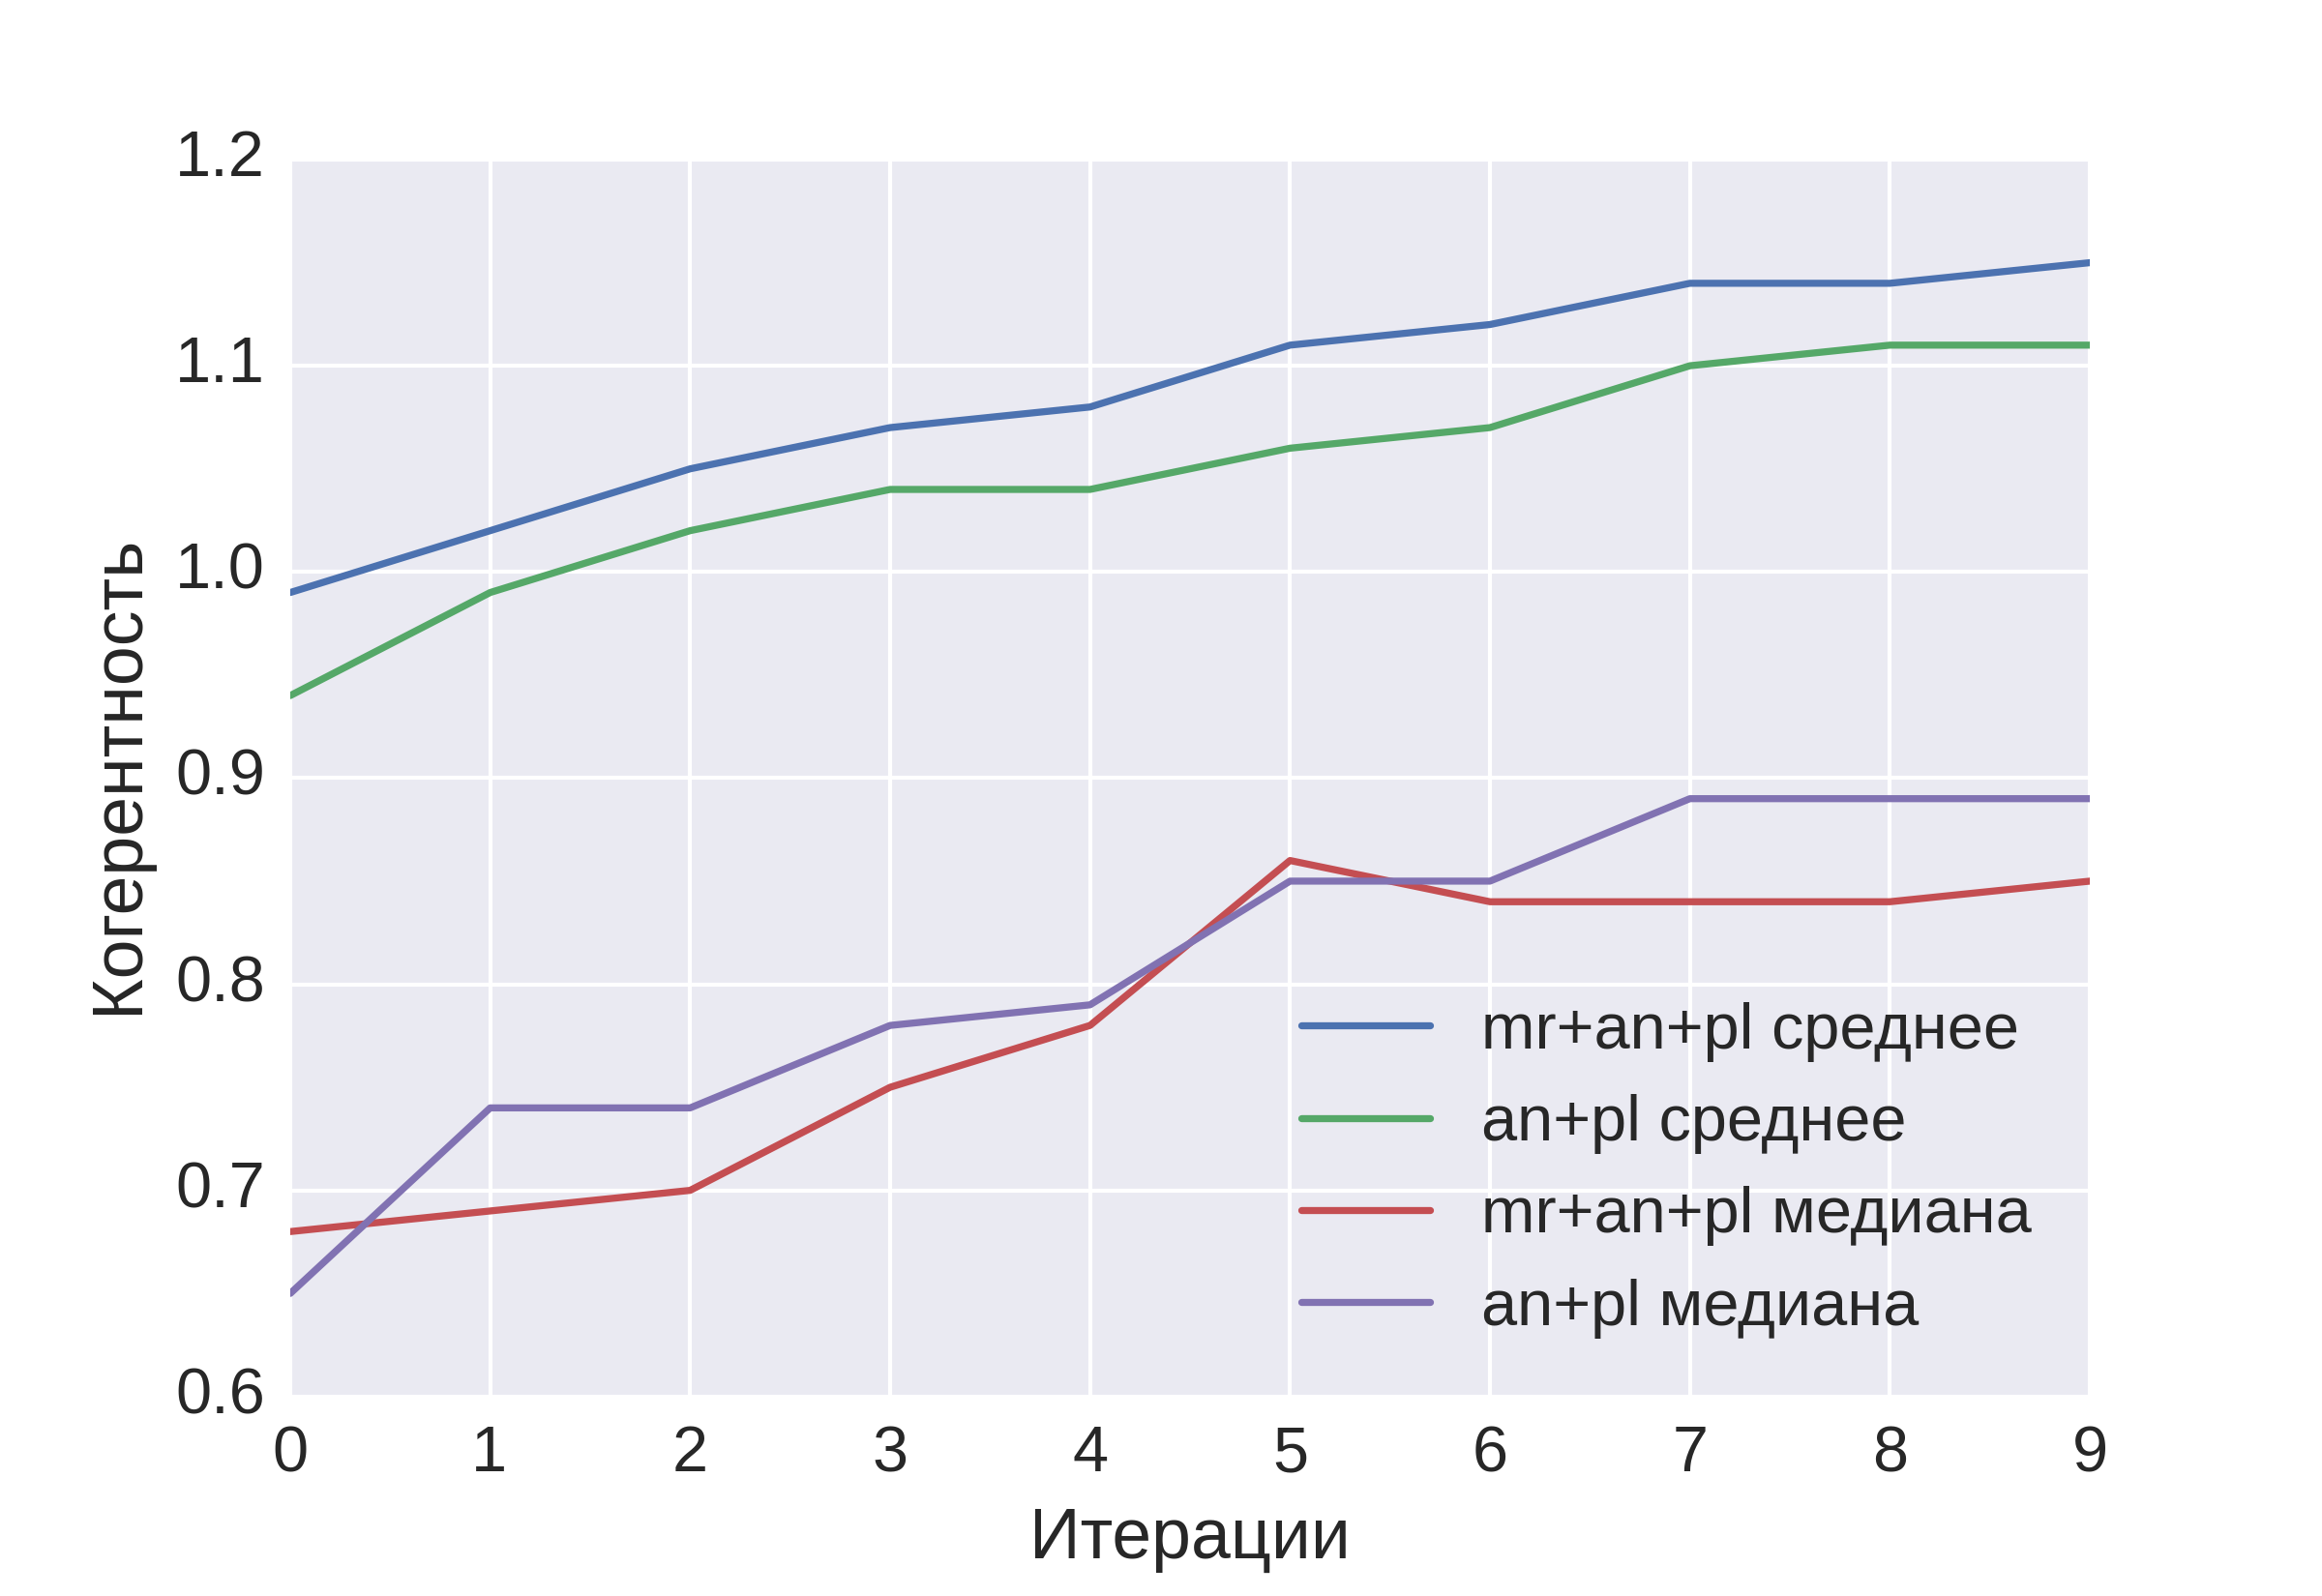
\includegraphics[scale=0.43]{img/no/3}
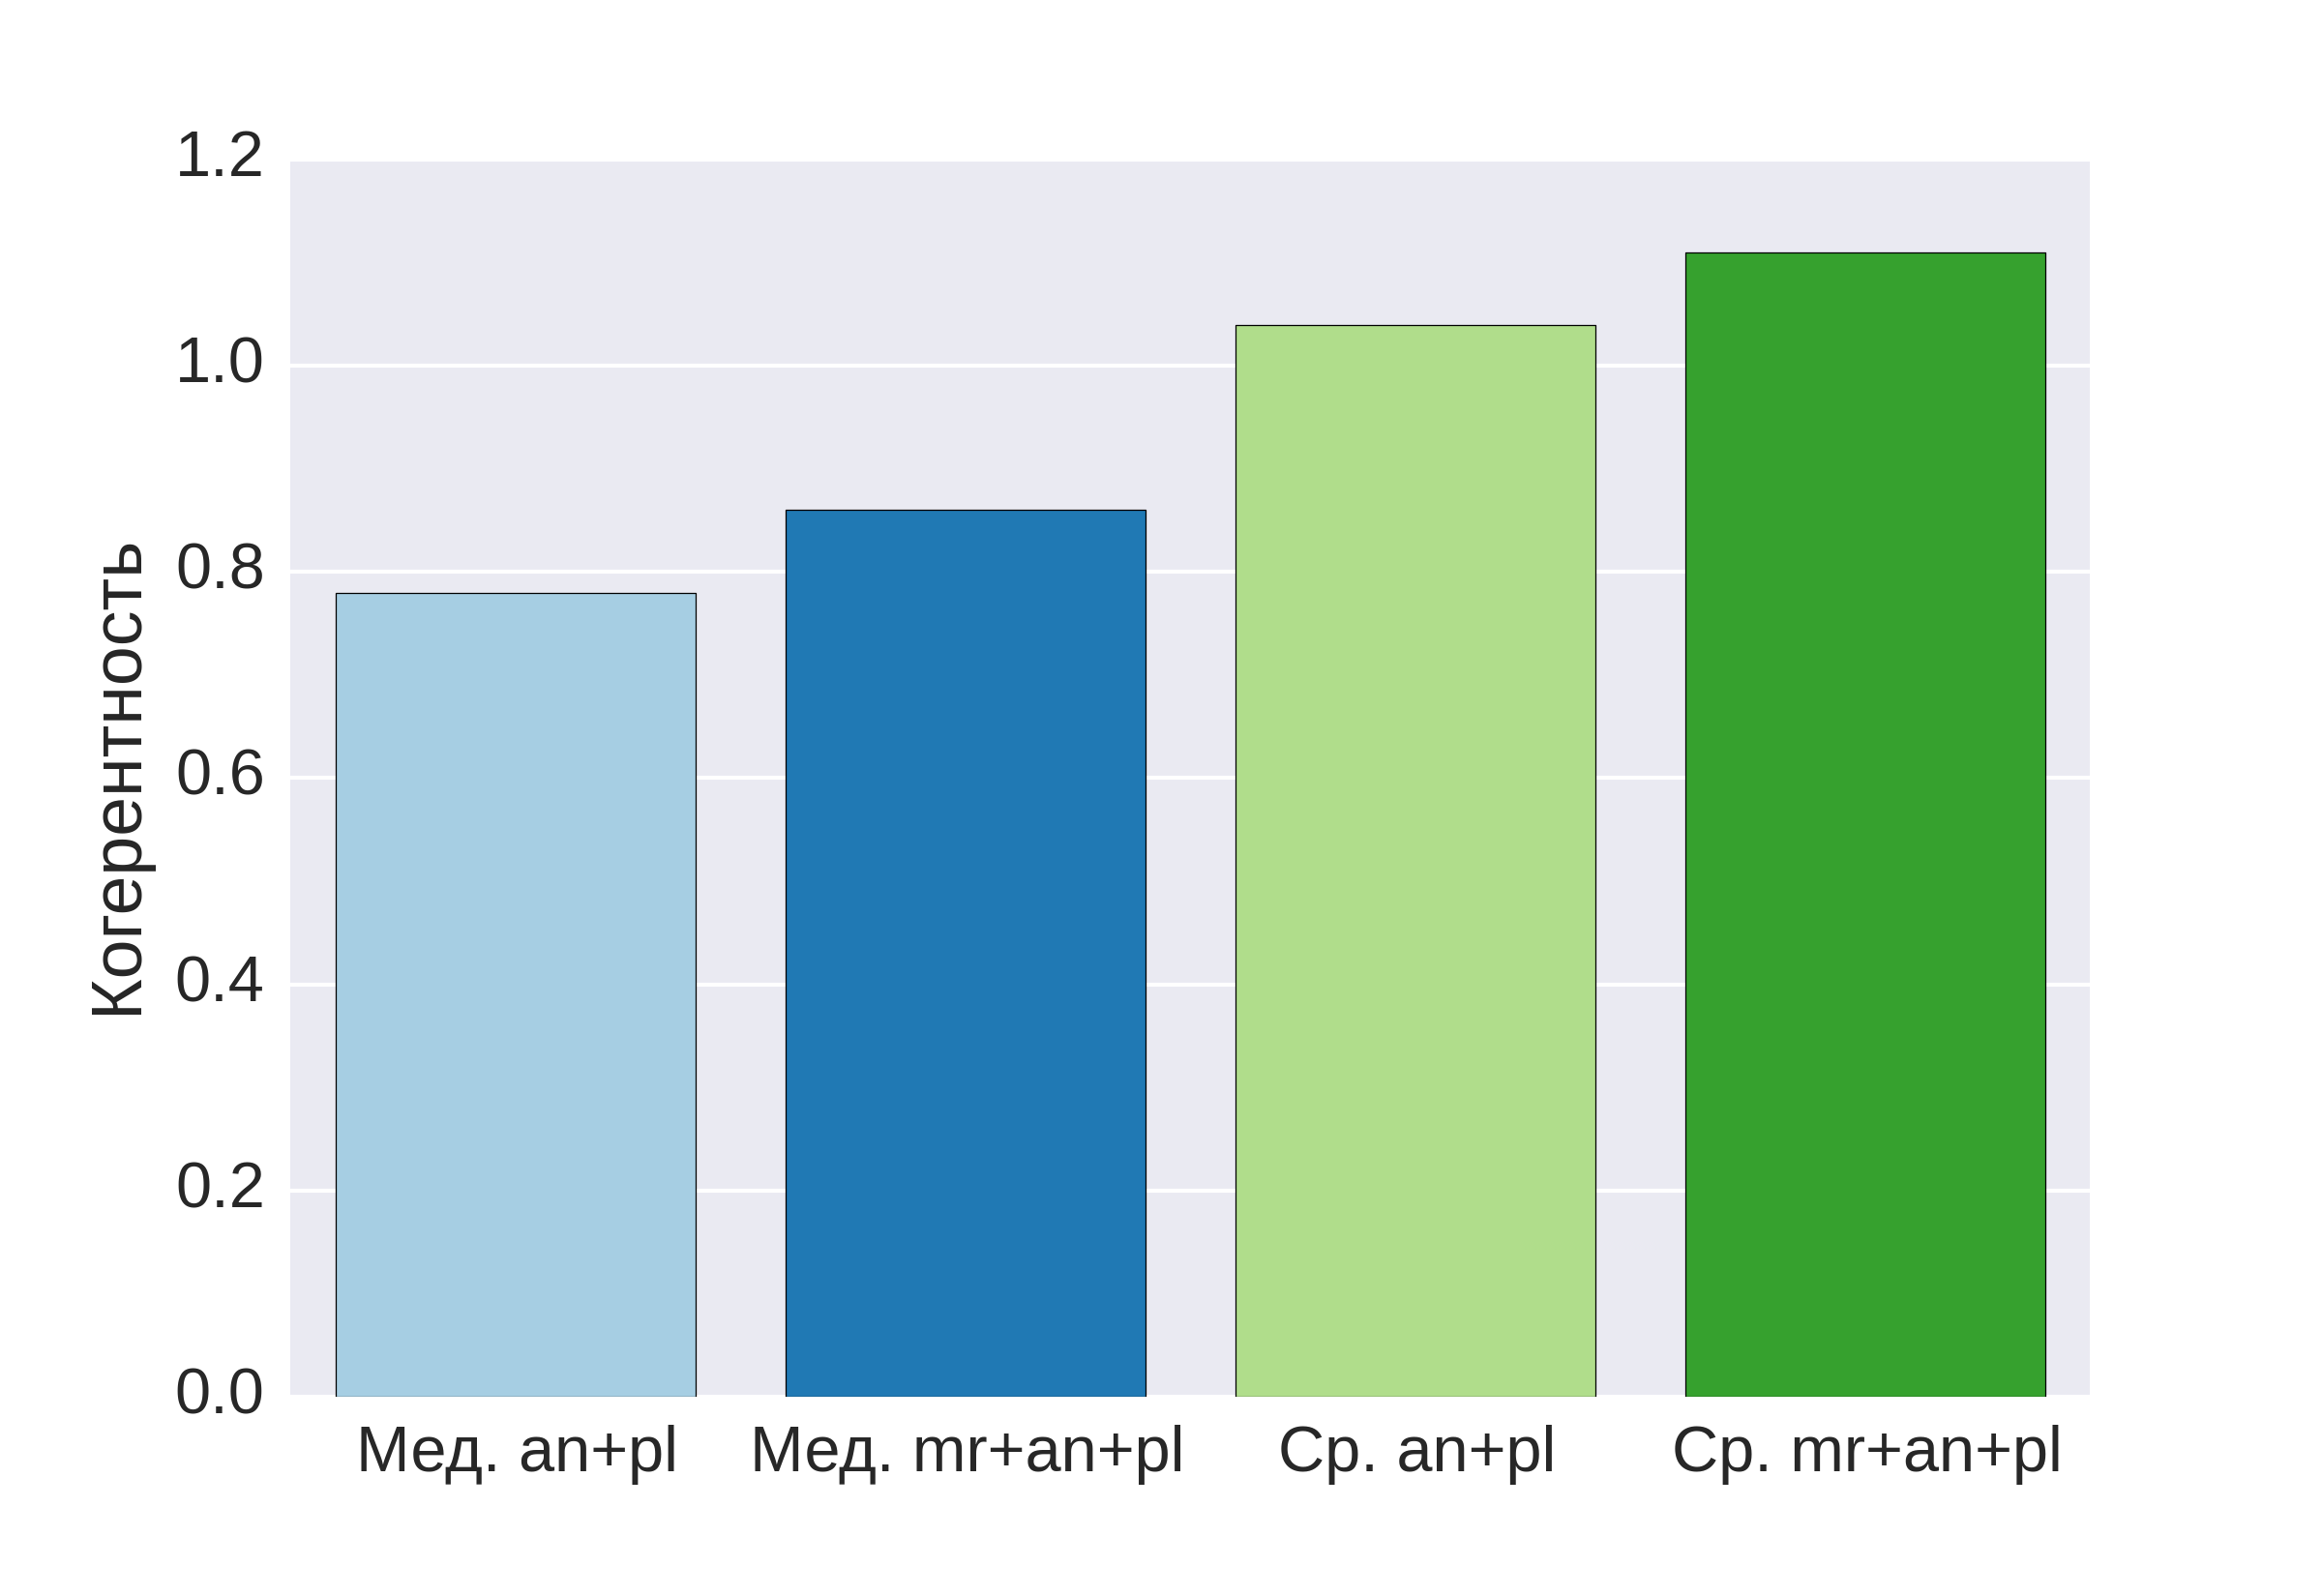
\includegraphics[scale=0.43]{img/no/6}\\
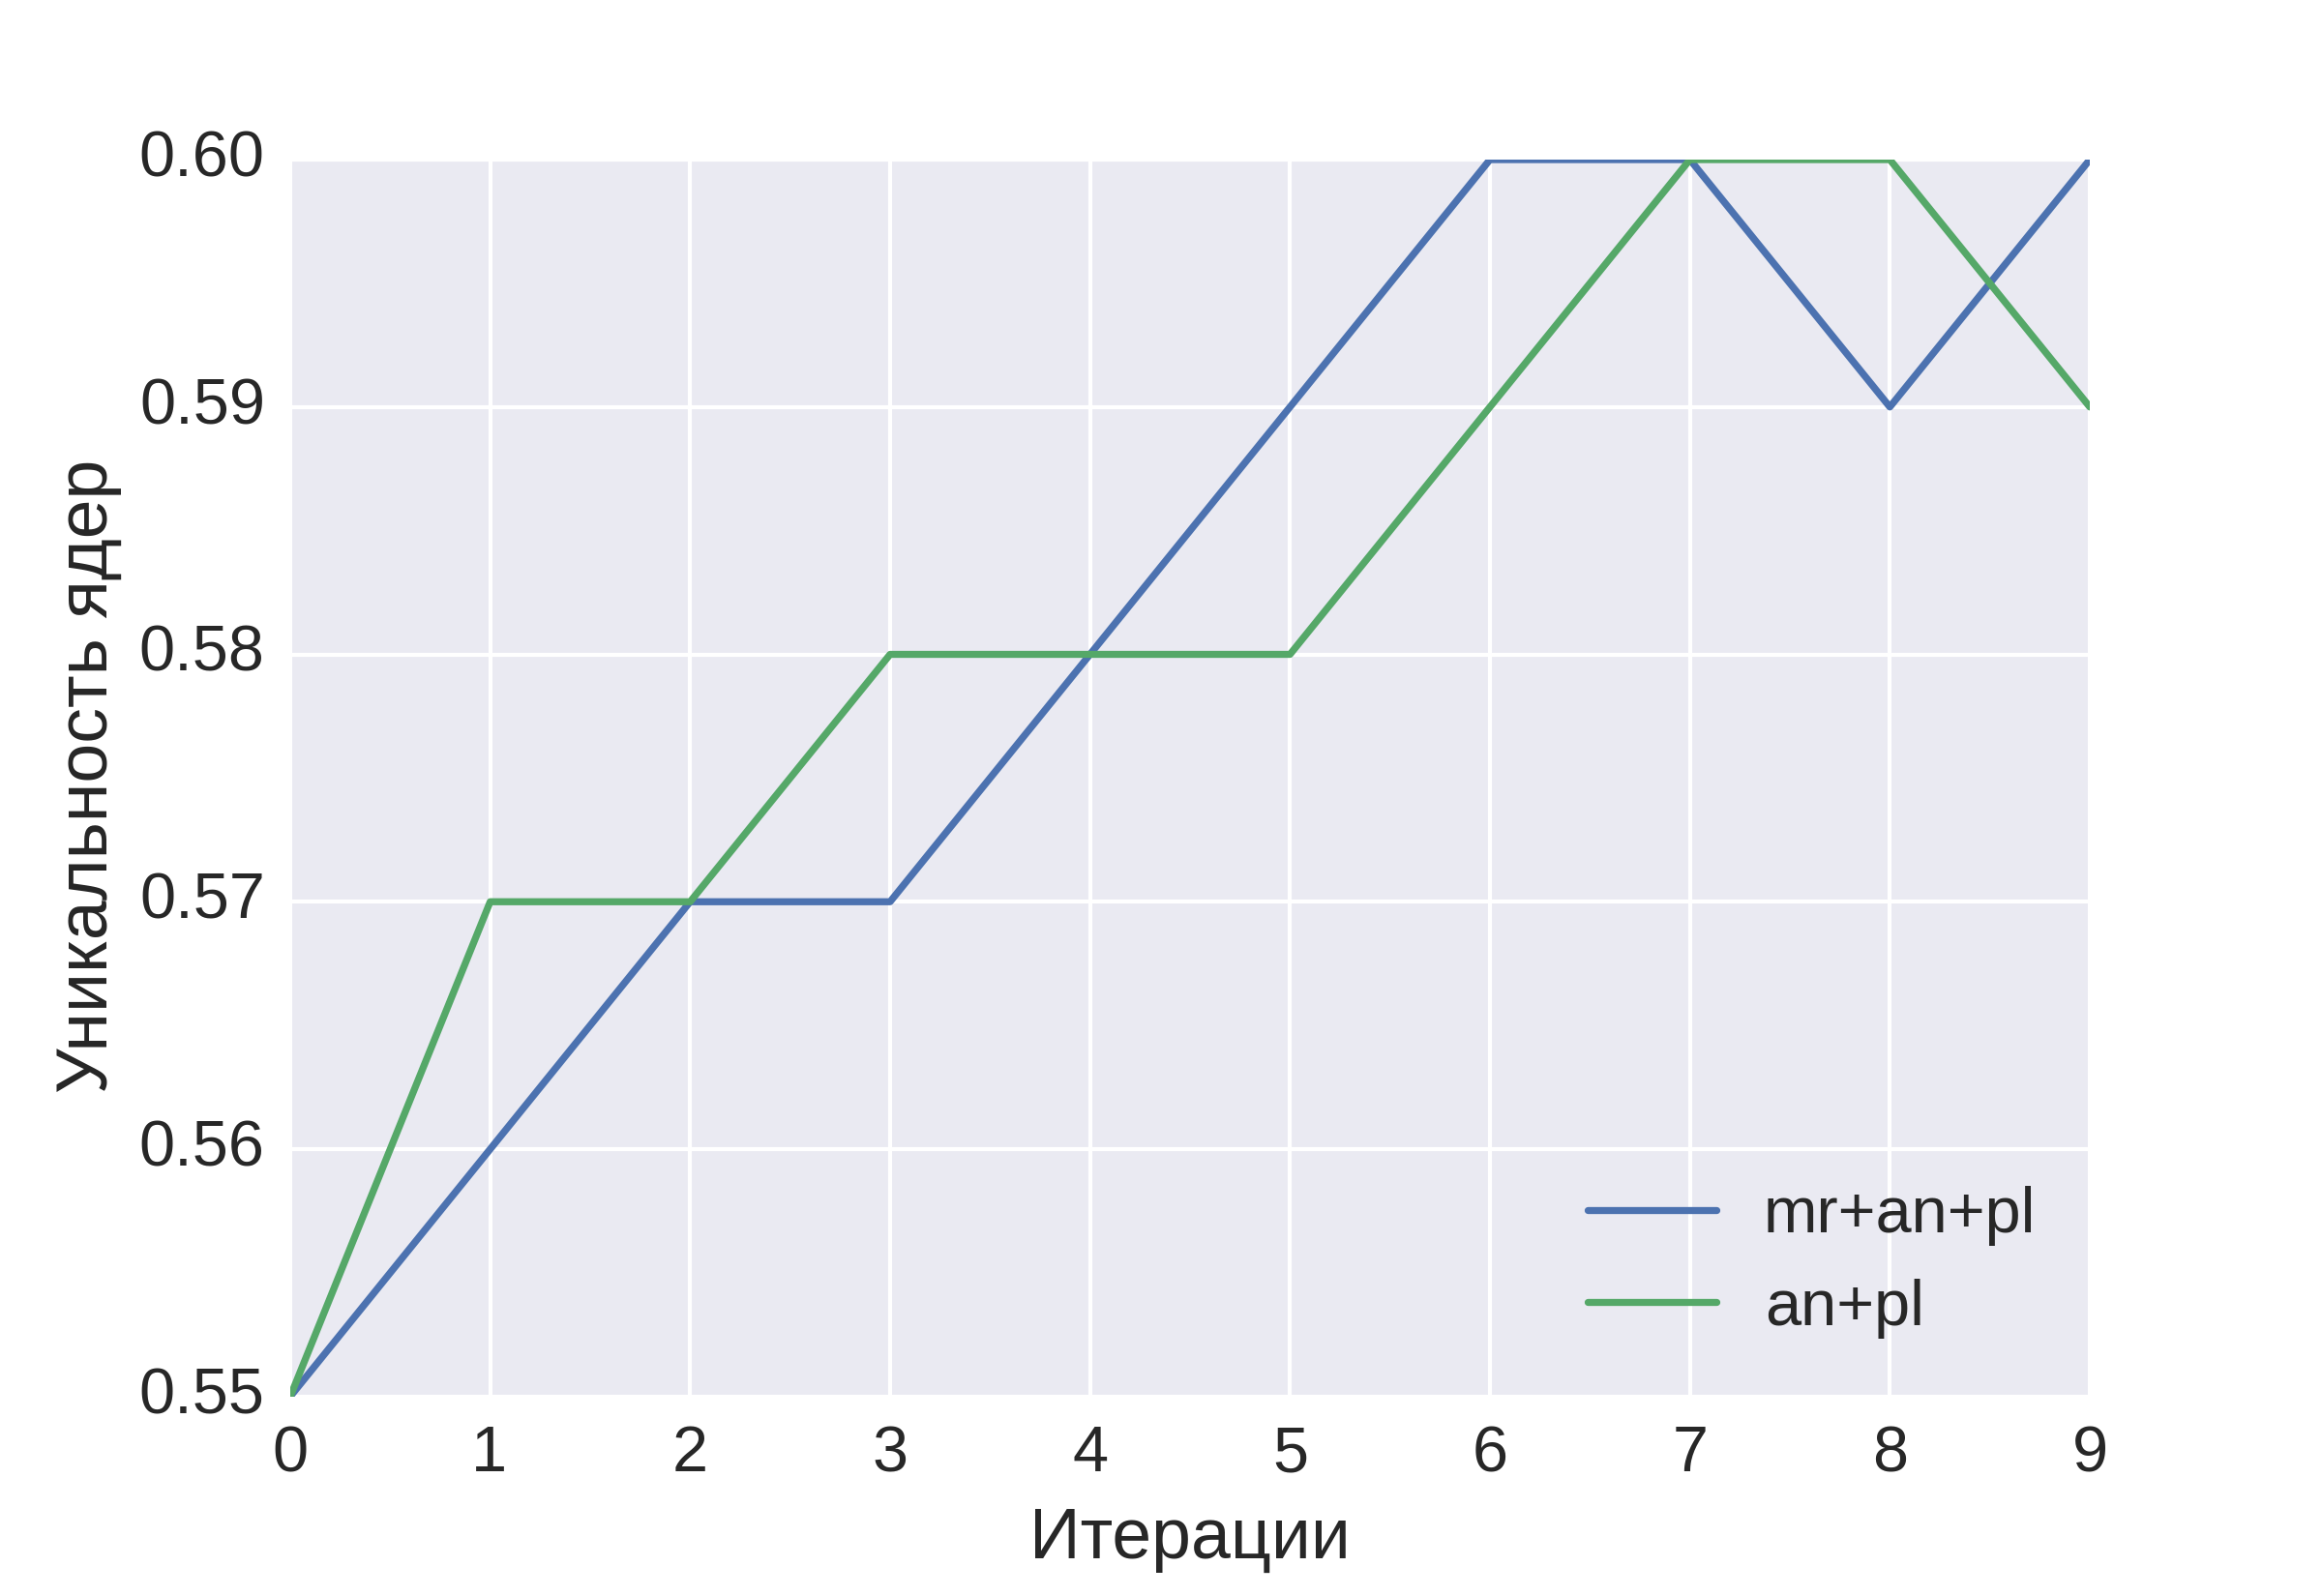
\includegraphics[scale=0.43]{img/no/4}
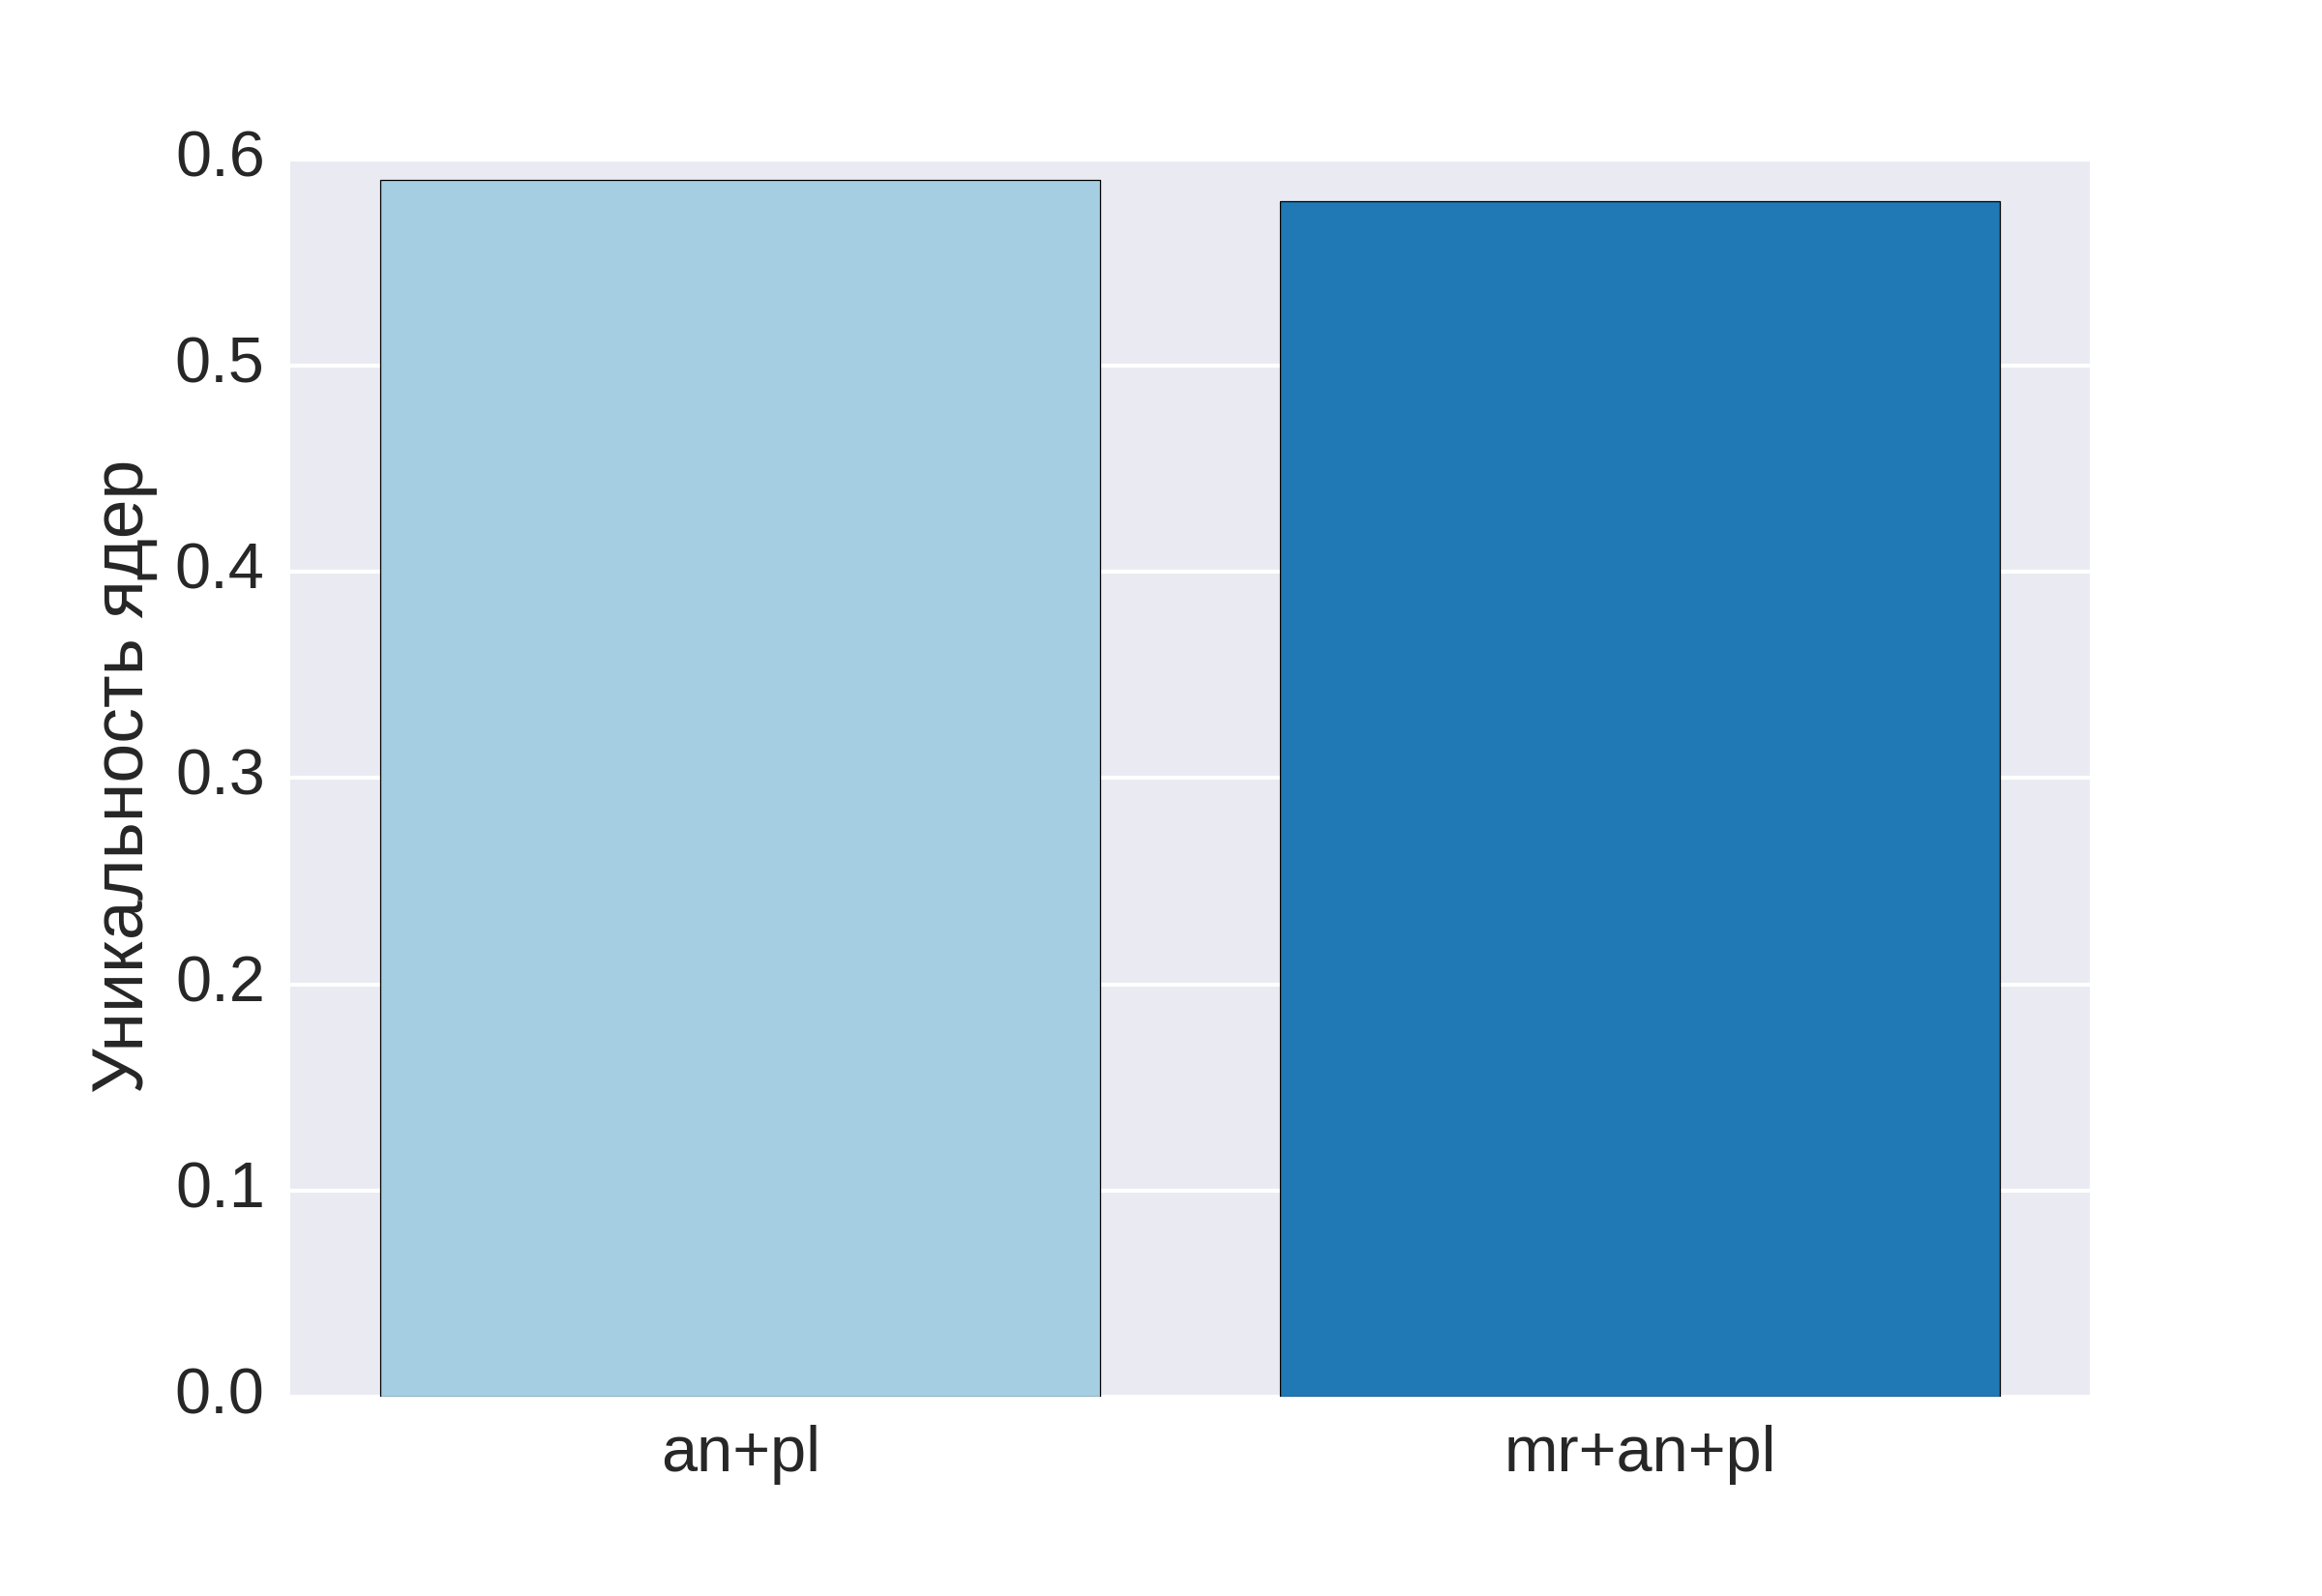
\includegraphics[scale=0.43]{img/no/7}
Рис. 11: Результаты экспериментов Комбинация PLSA и Anchor Words и учет морфологических ограничений.
		
\subsection{Учёт словосочетаний в Anchor Words}
Модель мешка слов совсем не учитывает порядок слов в документах, а на самом деле многие термины, употреблённые в тексте, употреблены именно в словосочетаниях и имеют совершенно другую тематическую окраску.

Добавление словосочетаний как уникальных элементов словаря существенно ухудшает перплексию, за сечёт увеличения размера словаря, но увеличивает интерпретируемость тем. Возникает вопрос --- можно ли учесть словосочетания в алгоритме Anchor Words, не добавляя их как уникальные элементы словаря?

\subsubsection*{Выделение словосочетаний (биграмм) }
Для выделения словосочетаний был использован метод предложенный в \cite{Dobrov2001}.

Авторы предлагают следующий алгоритм --- Если \emph{автор текста} использует некоторый термин, как отдельную единицу изложения, опирается на этот термин в своём изложении, то именно в этом тексте слова термина рядом будут встречаться чаще, чем в разбивку. Далее предполагается, что если пара слов встречается как непосредственные соседи более чем в половине случаев их появления в одном и том же текстовом окне, то это свидетельствует о том, что эта пара слов в совокупности служит автору опорной точкой, то есть представляет собой термин или фрагмент термина.

Для дальнейшего использования в тематических моделях предполагается использовать 1000 самых частотных биграмм.

\subsubsection*{Представление словосочетаний в Anchor Words}
Существует предположение, что биграммы точнее определяют тему, чем униграммы, поэтому возникла гипотеза, что биграммы будут хорошими якорными словами. Но добавление биграмм как уникальных элементов словаря ухудшает перплексию, поэтому был предложен следующий метод.

Обозначим $\textrm{B} = \{(w_1, w_2)_1,~\dots,~(w_1, w_2)_n\}$ -- множество биграмм,  $\textrm{W} =\{w_1, \dots, w_n\}$ -- вектора соответствующие терминам (в алгоритме \ref{recwt} ковариационная матрица слов), тогда представим каждую биграмму, как сумму векторов слов образующих данную биграмму -- $W(w_1)~+~W(w_2)$.
Произведём поиск якорных слов среди среди $$Q = \{q_1,~\dots,~q_n,~W(b_{11}) + W(b_{12}),~\dots,~W(b_{n1}) + W(b_{n1}))\},$$
после чего продолжим алгоритм \ref{recwt} без изменений. 

Проведённые эксперименты подтвердили данное предположение одновременным улучшением сразу нескольких метрик качества.

\subsubsection*{Эксперименты}

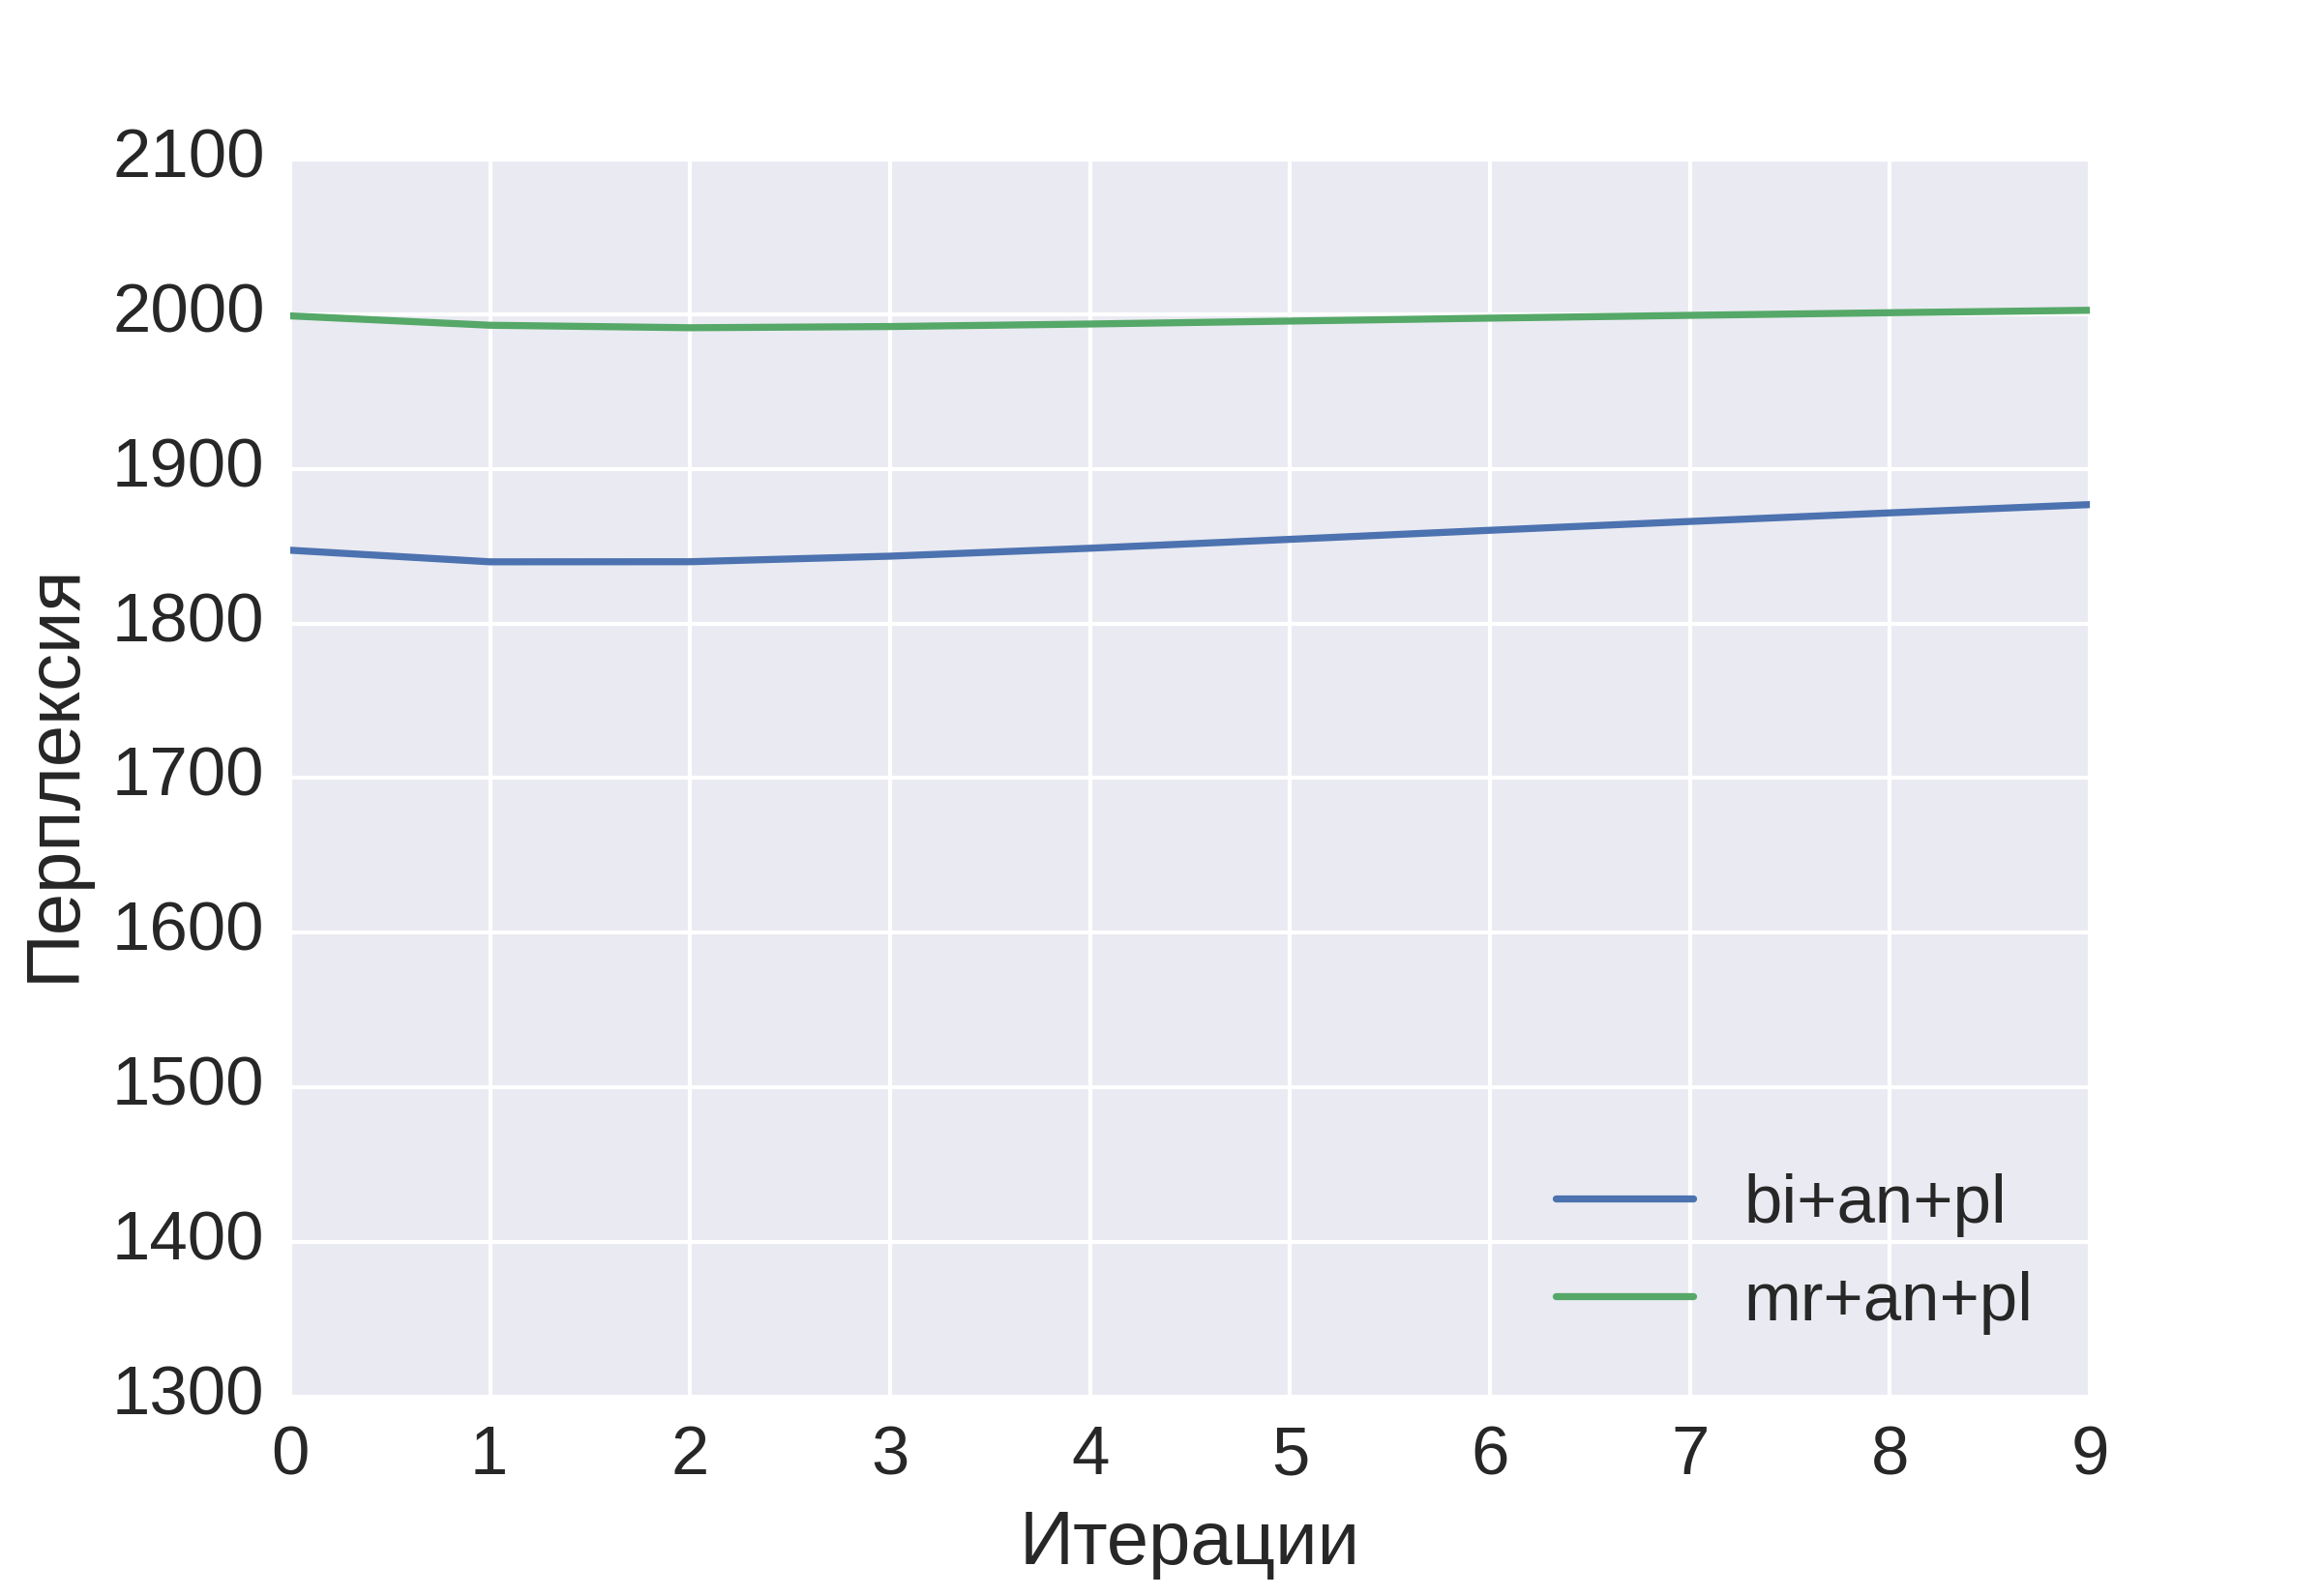
\includegraphics[scale=0.43]{img/bi/1}  
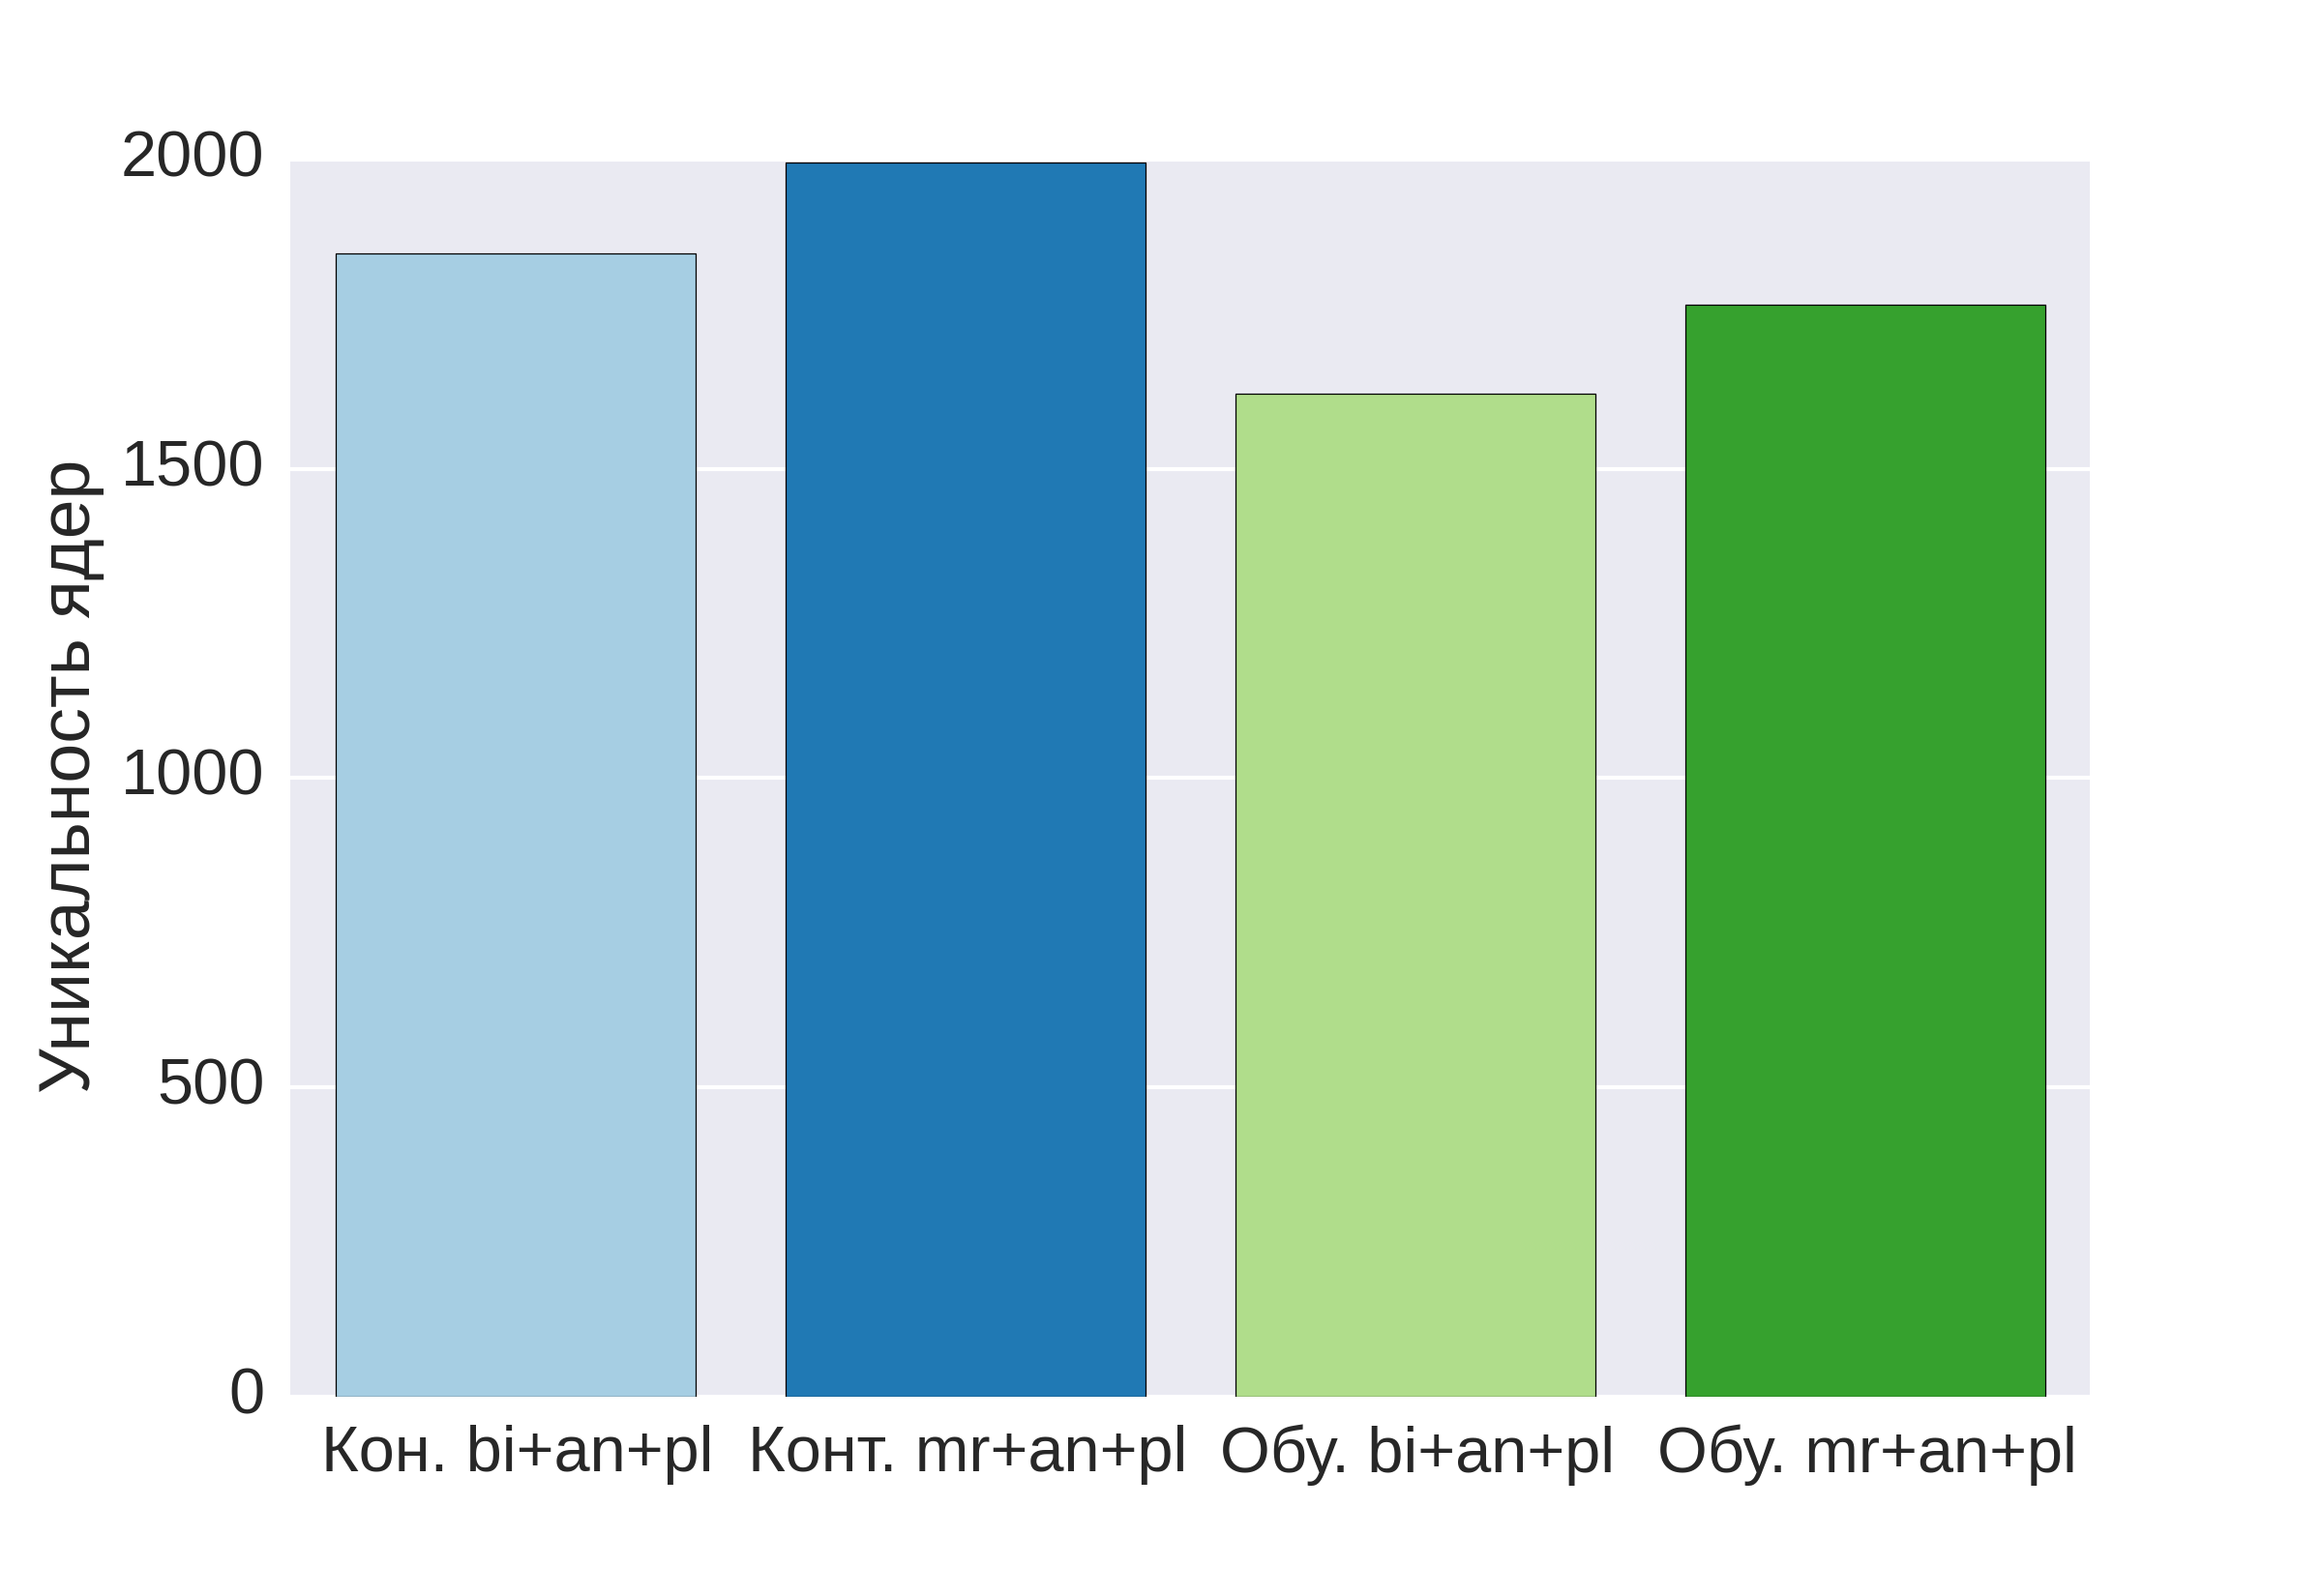
\includegraphics[scale=0.43]{img/bi/5}\\
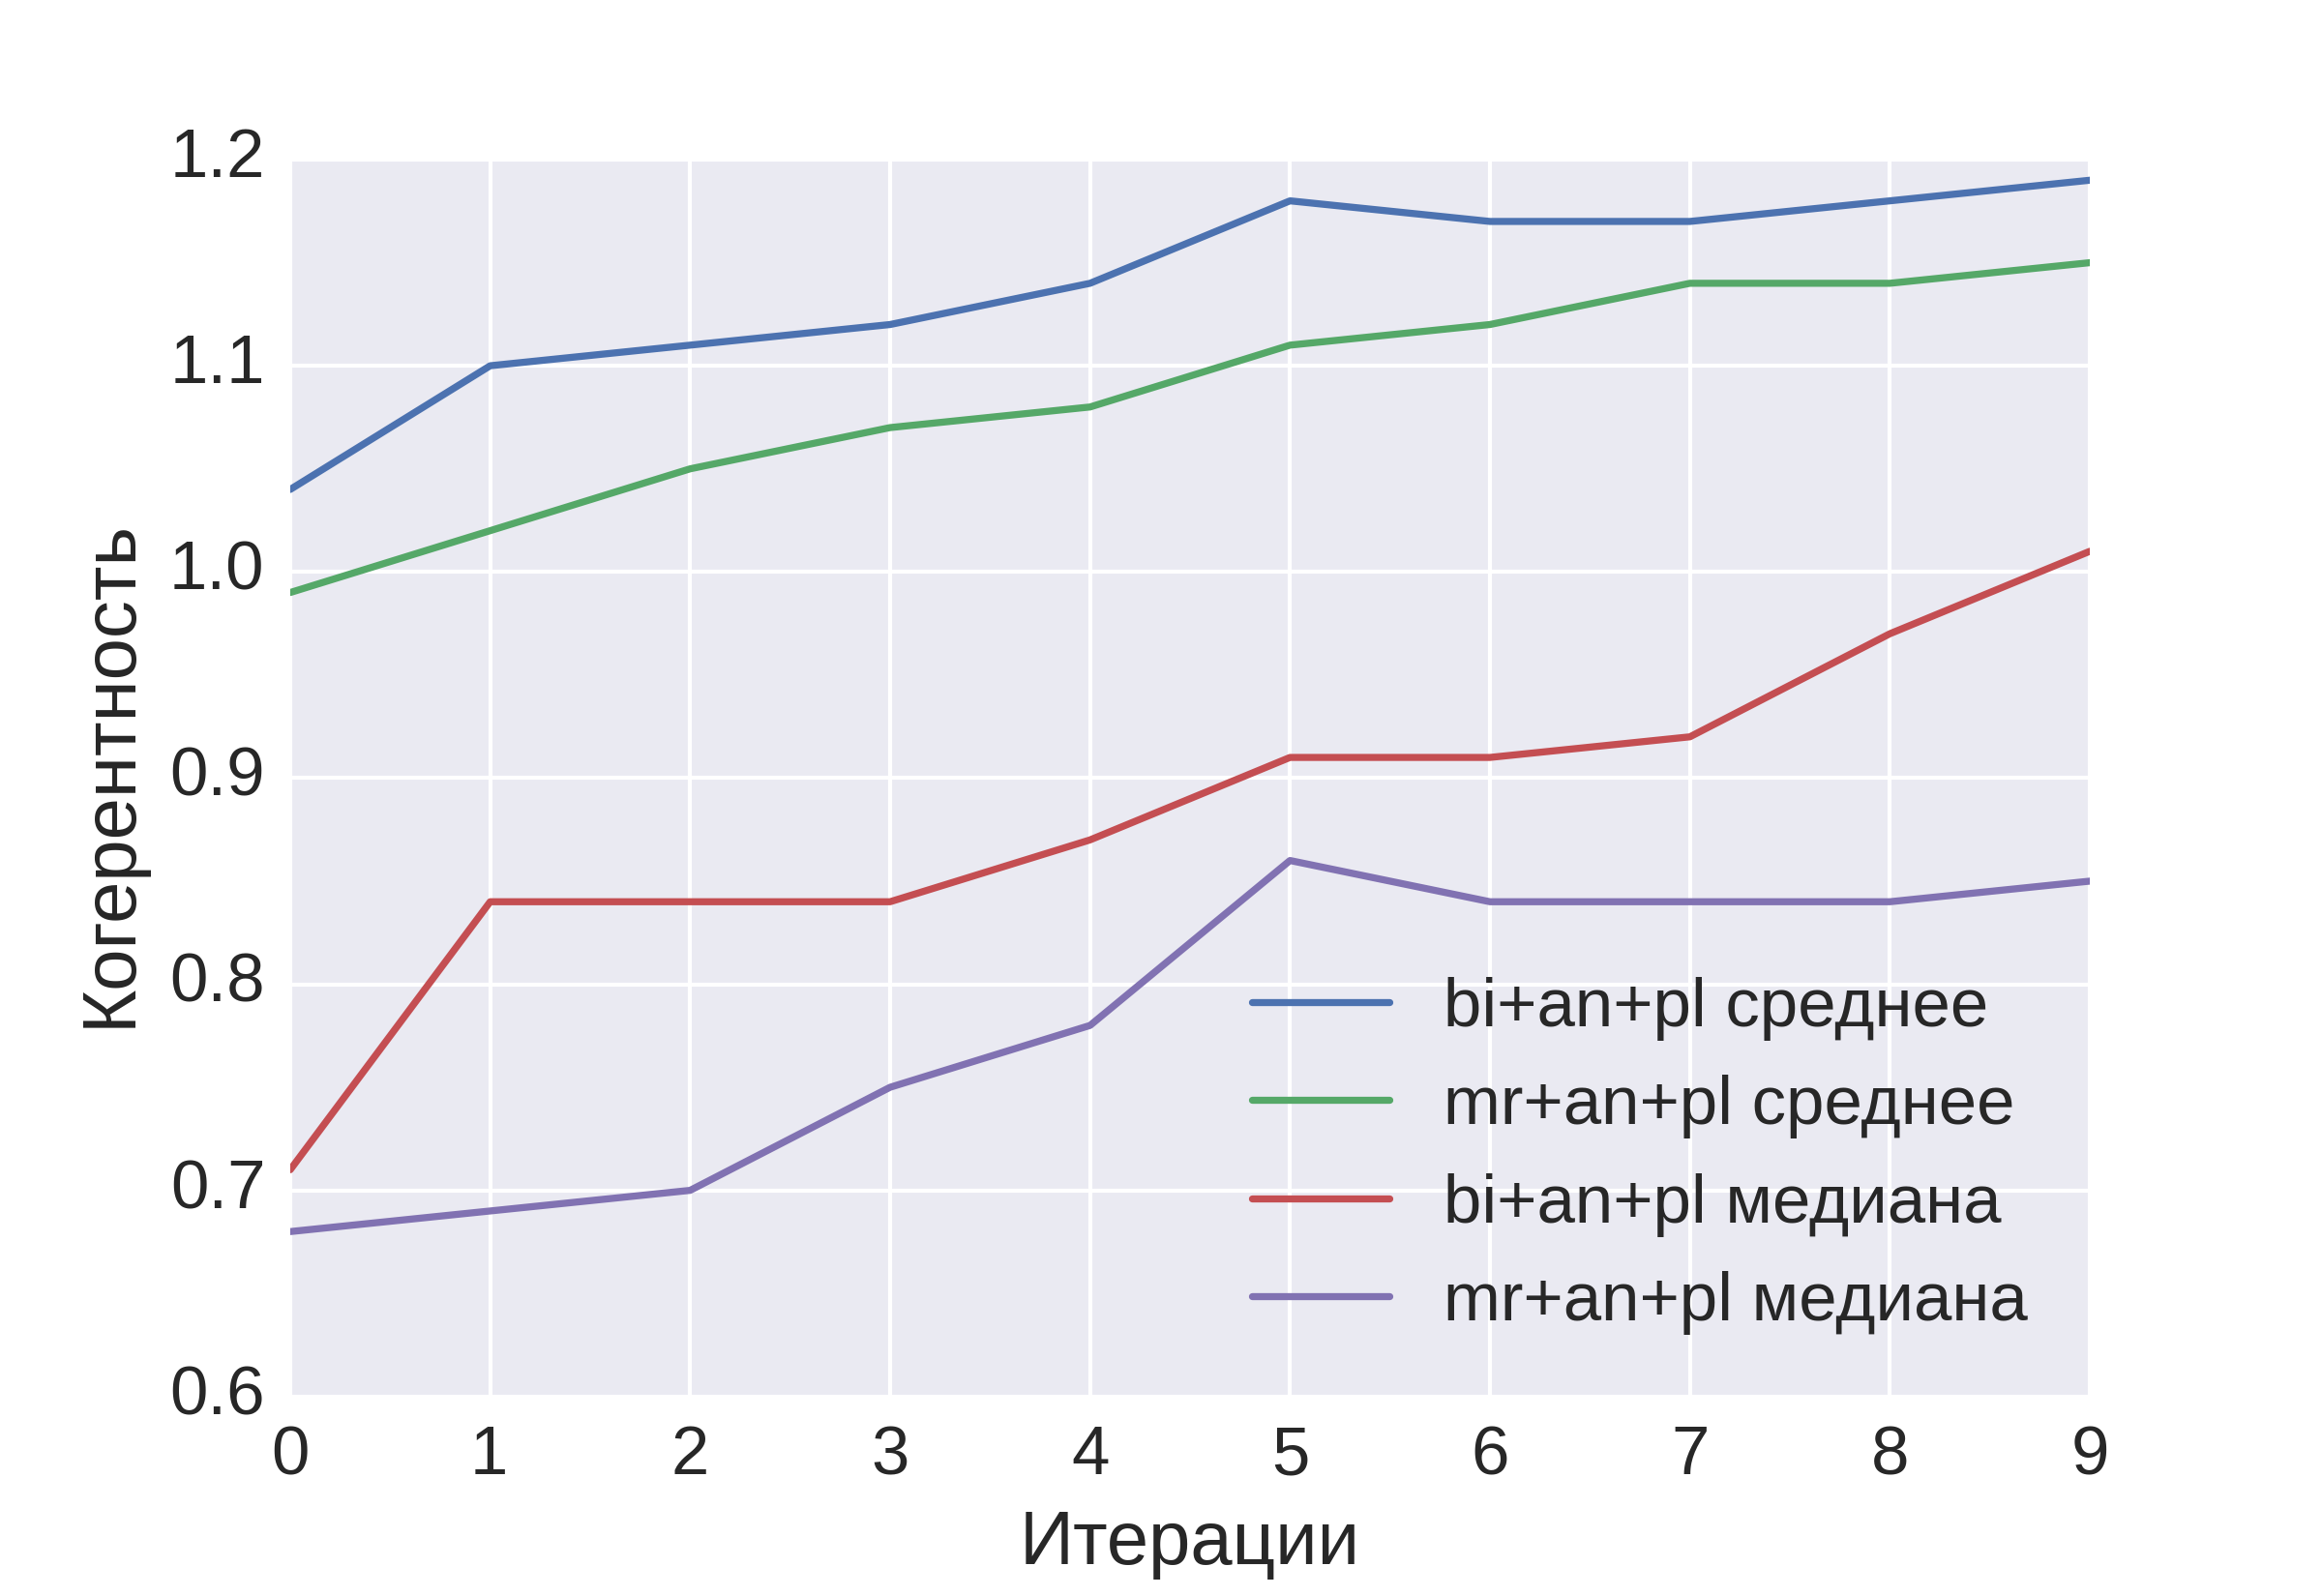
\includegraphics[scale=0.43]{img/bi/3}
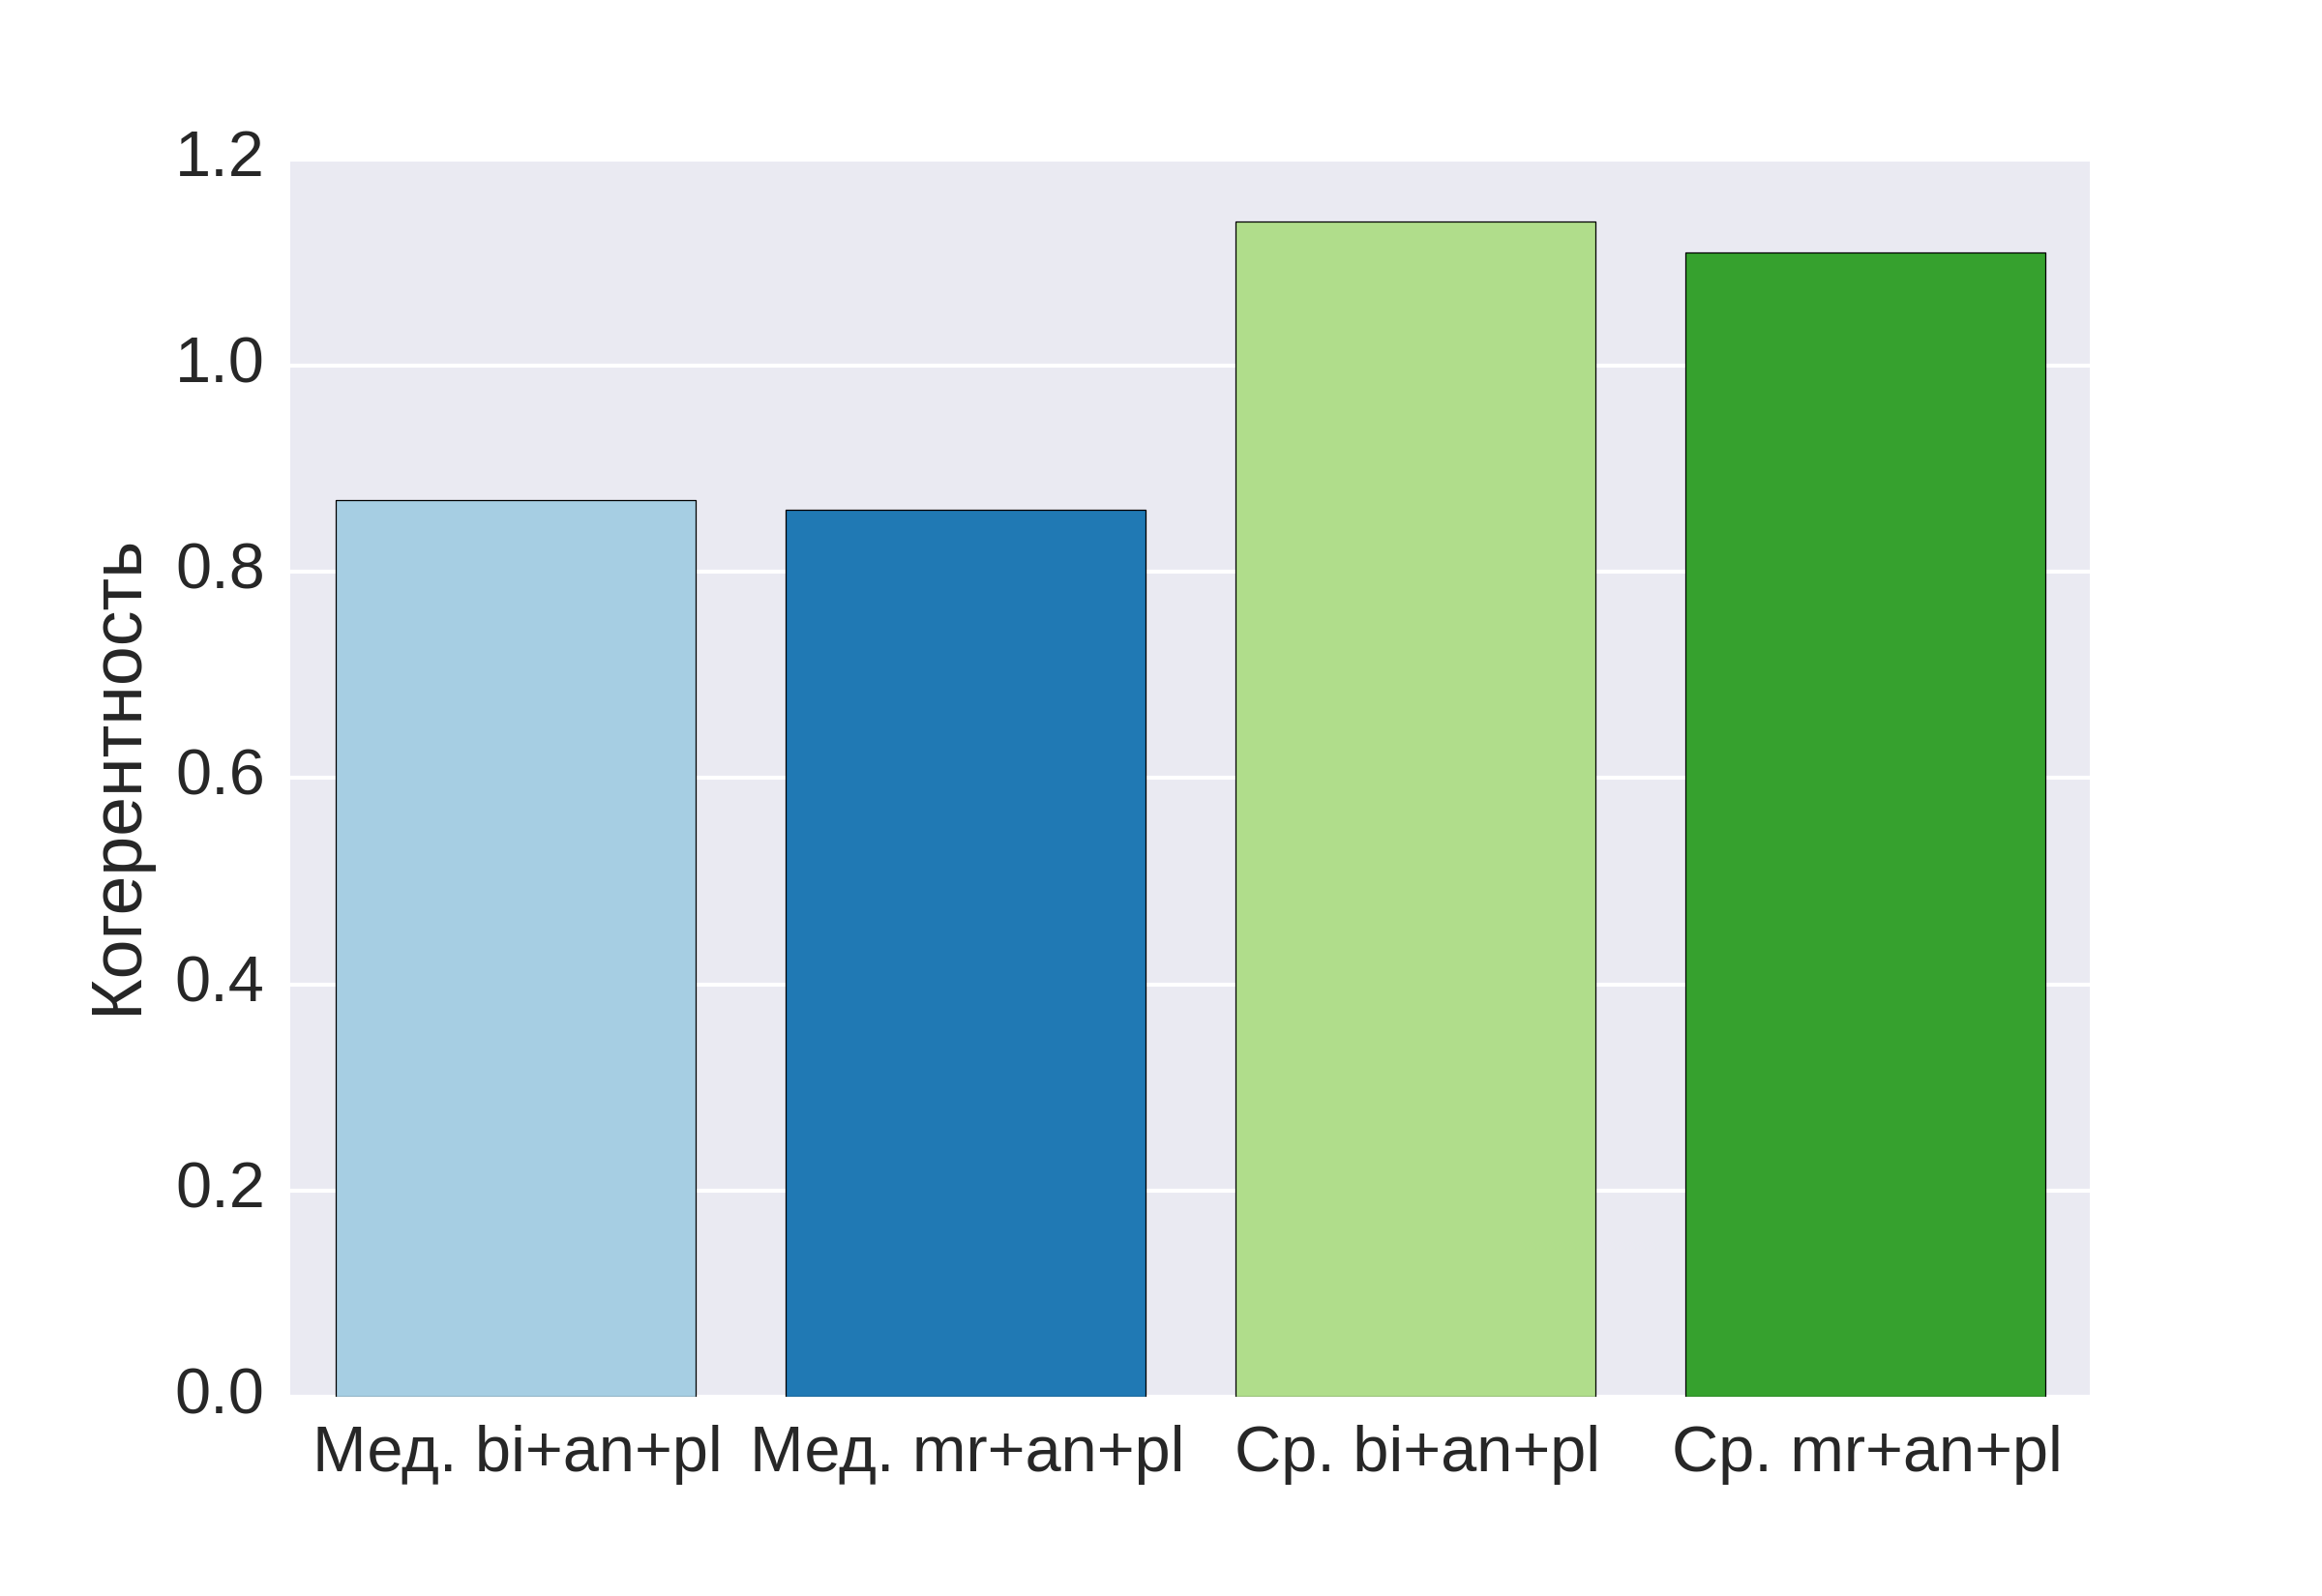
\includegraphics[scale=0.43]{img/bi/6}\\
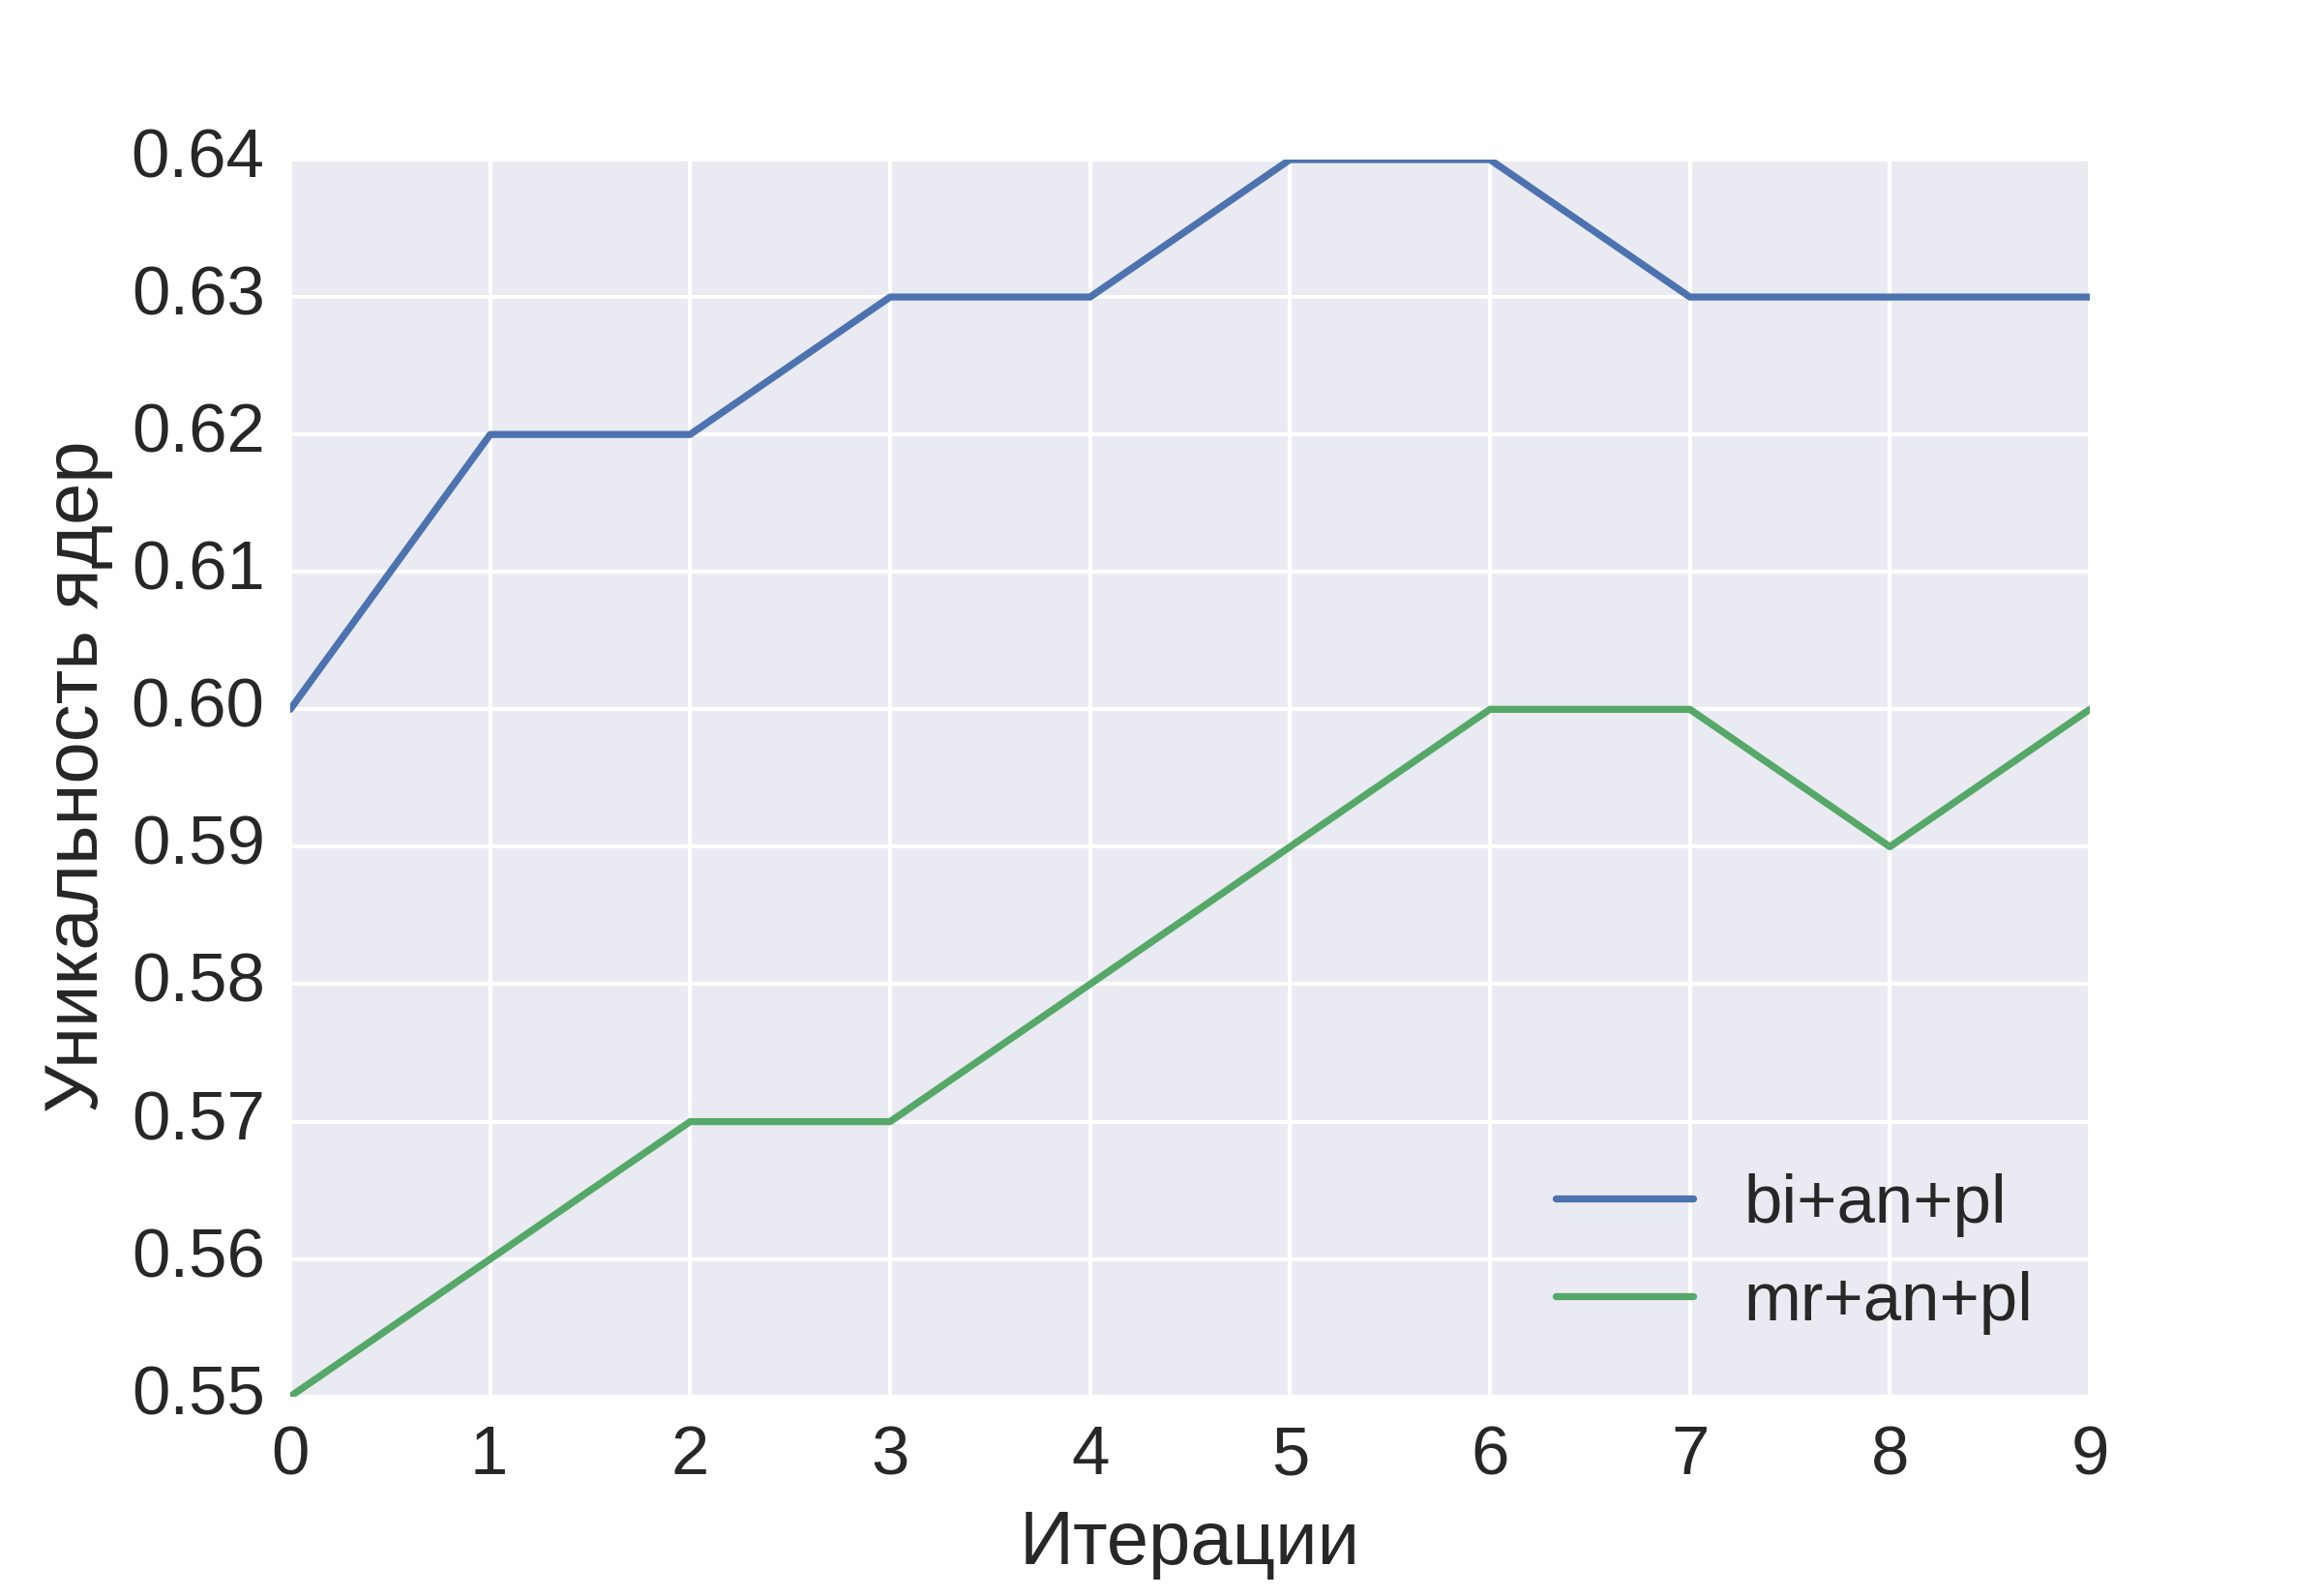
\includegraphics[scale=0.43]{img/bi/4}
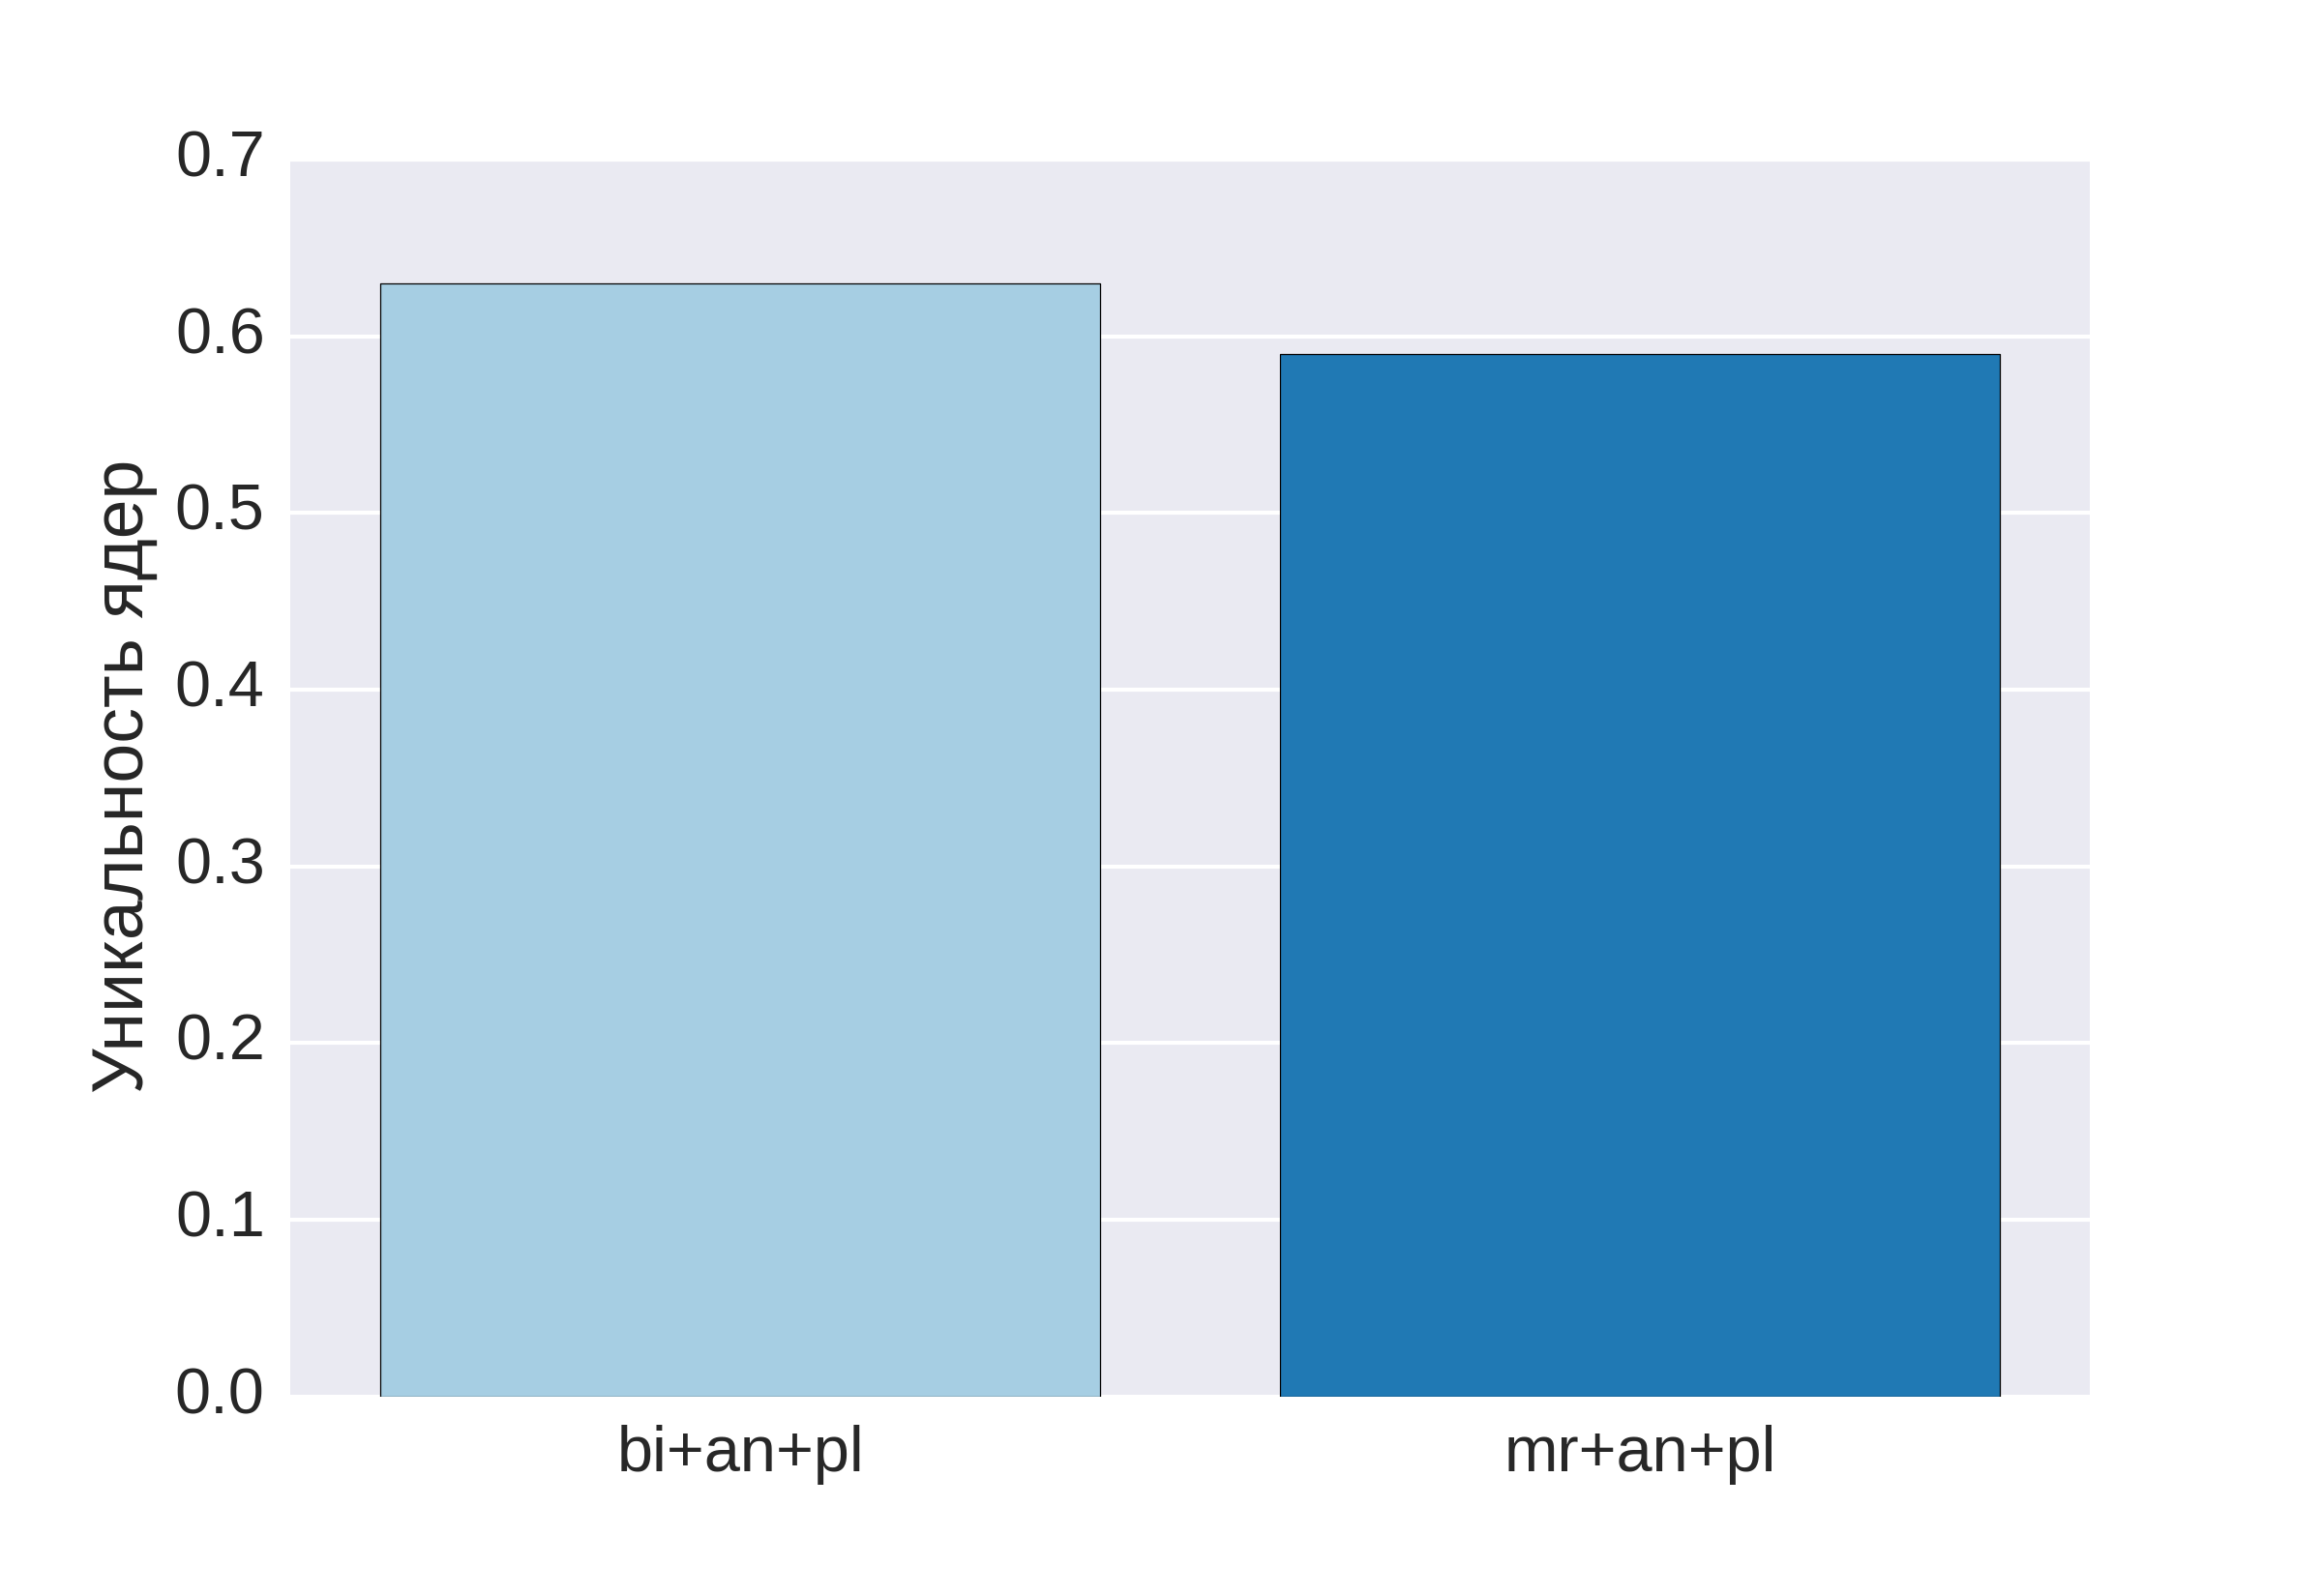
\includegraphics[scale=0.43]{img/bi/7}
Рис. 12: Результаты экспериментов Комбинация PLSA и Anchor Words и учет морфологических ограничений.

Хочется отметить, что при проведении экспериментов большинство якорных слов соответствовало биграммам.

\subsection{Сравнение результатов}
	В данном разделе результаты экспериментов объединены в одну таблицу \ref{srt}, легенда приведена около таблицы.
	
	Учёт лингвистических предположений дал заметное улучшение метрик качества, лучший результат показала комбинация \texttt{Anchor Words + PLSA + BIGRAMMS}, причём минимум перплексии достигался уже на первых итерациях PLSA, в следствии чего комбинация работала значительно быстрее, чем оригинальный PLSA. 
	
	Использование словосочетаний помогает улучшить качество тематических моделей, но все равно не учитывает большую часть информации. Безусловно будущее тематического моделирования -- отказ от гипотезы мешка слов. 
	
	Также, вполне разумным и эффективным является наложение лингвистических ограничений на якорные слова. 
	
	Полученные результаты, свидетельствуют о том, что для получения тематической модели хорошего качества, недостаточно одних частотных оценок. 
	
	Лингвистические особенности текста также важны, но учитывать такую информацию заметно сложнее. Дальнейшее развитие тематического моделирование несомненно заключается в отказе от гипотезы мешка слов.
	
	\begin{table}
		\centering
		\caption{Результаты работы алгоритмов}
		\label{srt}
	\begin{tabular}{|l|l|l|l|l|l|}
	\hline
	{\bf Алгоритм} & \multicolumn{2}{l|}{{\bf Перплексия}} & \multicolumn{2}{l|}{{\bf Когерентность}} & {\bf Уник. ядер} \\ \cline{2-5}
 	& обуч. & конт. & сред. & меди. &  \\ \hline
	\texttt{PL} &  1923& 2116&  0.95&   0.60&  0.40\\ \hline
	\texttt{AN} &  2099& 2330&  0.94&   0.63&  0.53\\ \hline
	\texttt{AN+PL} &  1822&  2052& 1.04&  0.78& 0.58\\ \hline
	\texttt{MR+AN+PL} & 1765& 1995& 1.11&  \textcolor{red}{0.86} &  \textcolor{red}{0.59}\\ \hline
	\texttt{BI+AN+PL} & \textbf{1621}& \textbf{1848}& \textbf{1.14}& \textbf{0.87}&  \textbf{0.63}\\ \hline
	\end{tabular}
	\end{table}

	\begin{itemize}
		\item {\tt PL} --- вероятностный латентный семантический анализ.
		\item {\tt AN} --- алгоритм якорных слов.
		\item {\tt MR} --- морфологические ограничения на якорные слова.
		\item {\tt BI} --- учёт словосочетаний.
		\item \textcolor{red}{красный} --- неустойчивый, \textbf{жирный} --- лучший результат.
	\end{itemize}


\newpage

\section*{Заключение}
\addcontentsline{toc}{section}{Заключение}

Для выполнения данной работы были изучены и реализованы стандартные модели \emph{тематического моделирования} PLSA и Anchor Words. 

\noindent Предложены подходы к:
\begin{enumerate}
	\item Внедрению морфологических ограничения в алгоритм Anchor Words 
	\item Учету словосочетаний в алгоритме Anchor Words 
	\item Введена метрика уникальности ядер
\end{enumerate}

\noindent Проведены эксперименты, показавшие улучшение метрик качества тематических моделей.
Полученные результаты показывают, что внедрение словосочетаний дало наибольший прирост, сразу по всем рассматриваемым метрикам качества.

В дальнейшем предполагается проверить работоспособность приведенных подходов на коллекциях текстов английского языка. 

\newpage

\newgeometry{left=0.5cm,bottom=0.1cm, top=0.5cm}

\addcontentsline{toc}{section}{Приложение} 

\begin{landscape}
	\begin{small}
		\begin{singlespace}
		
		\begin{table}[h]
		\centering
		\caption{Пример тем полученных алгоритмом PLSA}
		\label{my-label}
		\begin{tabular}{|l|l|}
		\hline
			Topic 0 &  денежный инфляция производство страна экономика экономический рост год цена \\ \hline
			Topic 1 &  объект фактор рубль сумма клиент оценка стоимость время факторинг \\ \hline
			Topic 2 &  налоговый рф орган налог ст налогоплательщик законодательство закон право \\ \hline
			Topic 3 &  стандарт международный финансовый страна год система национальный вопрос организация \\ \hline
			Topic 4 &  страна китай государственный сша система китайский доллар международный экономика \\ \hline
			Topic 5 &  бюджетный средство финансовый программа бюджет развитие федеральный проект государственный \\ \hline
			Topic 6 &  вклад страхование банковский система банка банк организация услуга депозит \\ \hline
			Topic 7 &  надзор банковский орган принцип надзорный банка капитал базель риска \\ \hline
			Topic 8 &  год бизнес банка банк розничный малое работать клиент развитие \\ \hline
			Topic 9 &  модель метод инновационный оценка анализ показатель являться уровень исследование \\ \hline
			Topic 10 &  реклама рекламный год говорить банка очень время продукт стать \\ \hline
			Topic 11 &  капитал средство экономика актив экономический собственный ресурс форма увеличение \\ \hline
			Topic 12 &  банка банк брэнд банкир год банковский очень клиент российский \\ \hline
			Topic 13 &  самый год отель самолт офшорный место километр мир трасса \\ \hline
			Topic 14 &  кредит банка рынок банк кредитование год потребительский агентство считать \\ \hline
			Topic 15 &  ассоциация россия кб банк банковский москва мурычев совет оао \\ \hline
			Topic 16 &  государственный система экономический наука защитить экономика библиогра назвый экон \\ \hline
			Topic 17 &  внутренний контроль организация управление система аудит подразделение служба внешний \\ \hline
			Topic 18 &  монета денежный обращение россия рубль год деньга реформа золото \\ \hline
			Topic 19 &  сотрудник работа персонал система обучение специалист программа управление документ \\ \hline
			Topic 20 &  деньга стоимость цена товар оценка компания рыночный функция денежный \\ \hline
		\end{tabular}
		\end{table}
	
		\end{singlespace}
	\end{small}
\end{landscape}

\newpage
\begin{landscape}
	\begin{small}
		\begin{singlespace}
			\begin{table}[h]
			\centering
			\caption{Пример тем полученных алгоритмом Anchor Words}
			\label{my-label}
				\begin{tabular}{|l|l|}
				\hline
				москва &   москва банка банк ооо россия лицензия номер регистрация \\ \hline
				налоговый &   налоговый налог рф ст налогоплательщик порядок уплата сумма \\ \hline
				история &   кредитный история бюро информация организация замщик закон банка \\ \hline
				нормативный &   банка россия нормативный закон банковский надзор деятельность федеральный \\ \hline
				председатель &   председатель правление банк оао кб зао акб главный \\ \hline
				основание &   организация кредитный россия основание государственный банка управление регион \\ \hline
				важный &   важный потребитель доверие завоевание упрочение связь время являться \\ \hline
				валюта &   валюта рубль курс иностранный национальный использовать банк капитал \\ \hline
				управлять &   компания управлять адрес год решение фактический требование телефон \\ \hline
				рабочий &   рабочий время работа неделя норма группа труд работник \\ \hline
				ставка &   ставка процентный рефинансирование уровень депозит цб годовой снижение \\ \hline
				отчтность &   отчтность финансовый мсфо организация бухгалтерский аудит аудитор вопрос \\ \hline
				страхование &   страхование страховой страхов страховщик обязательный премия участник компания \\ \hline
				опыт &   опыт международный страна рынок работа тема поддержка иностранный \\ \hline
				акция &   акция рынок размещение акционер инвестор капитал фондовый биржа \\ \hline
				сила &   россия банка сила изменение указание официальный год положение \\ \hline
				платж &   платж система платжный счт расчт карта средство услуга \\ \hline
				ассоциация &   ассоциация банковский банк россия российский президент банка арба \\ \hline
				защита &   защита система информация решение отношение безопасность право дать \\ \hline
				юридический &   лицо юридический физический счт реестр деятельность сведение право \\ \hline
				фонд &   фонд пенсионный негосударственный пенсия год накопление средство тысяча \\ \hline
				\end{tabular}
			\end{table}
		\end{singlespace}
	\end{small}
\end{landscape}

\begin{landscape}
	\begin{small}
		\begin{singlespace}
			\begin{table}[h]
			\centering
			\caption{Пример тем полученных алгоритмом \\ Anchor Words + PLSA}
			\label{my-label}
				\begin{tabular}{|l|l|}
				\hline
				москва &  москва ооо кб оао банк банка адрес зао номер \\ \hline
				налоговый &  налоговый налог ст рф налогоплательщик налогообложение уплата кодекс порядок \\ \hline
				история &  кредитный история информация замщик бюро закон организация риск запрос \\ \hline
				нормативный &  банка закон надзор федеральный деятельность порядок нормативный банковский акт \\ \hline
				председатель &  председатель правление оао александр владимир главный банк зао кб \\ \hline
				основание &  организация кредитный основание государственный регион внести управление приказ регистрация \\ \hline
				важный &  важный потребитель доверие время должный канал необходимый позволять особенно \\ \hline
				валюта &  рубль валюта курс иностранный национальный использовать укрепление капитал евро \\ \hline
				управлять &  компания управлять управление решение год инвестиционный фактический ук требование \\ \hline
				рабочий &  рабочий работник труд время работа трудовой женщина выходной продолжительность \\ \hline
				ставка &  ставка процентный уровень рефинансирование снижение инфляция ликвидность депозит высокий \\ \hline
				отчтность &  отчтность мсфо финансовый оценка бухгалтерский информация составление организация должный \\ \hline
				страхование &  страхование страховой страхов страховщик обязательный премия компания выплата тариф \\ \hline
				опыт &  страна международный рынок опыт работа развивающийся поддержка иностранный германия \\ \hline
				акция &  акция рынок размещение акционер инвестор фондовый биржа доля втб \\ \hline
				сила &  россия сила изменение банка положение указание официальный год внесение \\ \hline
				платж &  платж платжный расчт система счт карта средство услуга использование \\ \hline
				ассоциация &  ассоциация банковский президент арба банк российский развитие региональный россия \\ \hline
				защита &  защита система отношение безопасность информация решение доступ дать угроза \\ \hline
				юридический &  лицо юридический физический счт право сведение реестр форма деятельность \\ \hline
				фонд &  фонд пенсионный пенсия негосударственный накопление средство обеспечение инвестиционный год \\ \hline
				\end{tabular}
			\end{table}
		\end{singlespace}
	\end{small}
\end{landscape}

\begin{landscape}
	\begin{small}
		\begin{singlespace}
			\begin{table}[h]
			\centering
			\caption{Пример тем полученных алгоритмом \\ Anchor Words + PLSA + Morph}
			\label{my-label}
				\begin{tabular}{|l|l|}
				\hline
				москва &  москва банк банка россия оао ооо адрес кб зао \\ \hline
				история &  кредитный история информация бюро замщик закон организация отчт запрос \\ \hline
				затрата &  затрата метод управленческий необходимый продукция использовать себестоимость дать производственный \\ \hline
				председатель &  председатель правление банк оао александр владимир кб зао московский \\ \hline
				основание &  организация кредитный основание россия государственный внести следующий регистрация приказ \\ \hline
				осуществление &  банковский банк операция осуществление кредитный россия банка лицензия организация \\ \hline
				миллиард &  миллиард рубль миллион составить увеличиться сумма актив средство доля \\ \hline
				связь &  связь важный потребитель мера россия доверие учитывать общественный внешний \\ \hline
				страхование &  страхование страховой страхов страховщик обязательный премия выплата вид тариф \\ \hline
				валюта &  валюта валютный рубль курс денежный иностранный центральный национальный резерв \\ \hline
				опыт &  международный рынок страна опыт банк развивающийся тема германия иностранный \\ \hline
				отчтность &  отчтность бухгалтерский финансовый мсфо учт аудитор аудиторский учтный организация \\ \hline
				фонд &  фонд пенсионный пенсия управлять накопление негосударственный инвестиционный средство инвестирование \\ \hline
				ставка &  ставка процентный рефинансирование ликвидность уровень рынок снижение депозит инфляция \\ \hline
				сила &  россия сила изменение банка положение указание год официальный порядок \\ \hline
				ассоциация &  ассоциация банковский банк россия арба российский президент сообщество региональный \\ \hline
				филиал &  филиал банка банк кредитный офис сбербанк миллион отделение открытие \\ \hline
				защита &  защита система безопасность дать обеспечение информация проблема решение доступ \\ \hline
				акция &  акция размещение акционер инвестор фондовый предложение доля пакет приобретение \\ \hline
				рабочий &  рабочий работник труд время трудовой женщина место часы мужчина \\ \hline
				совет &  совет деятельность россия принять минфин заседание комитет вопрос ответственный \\ \hline
				
		
				\end{tabular}
			\end{table}
		\end{singlespace}
	\end{small}
\end{landscape}

\begin{landscape}
	\begin{small}
		\begin{singlespace}
			\begin{table}[h]
			\centering
			\caption{Пример тем полученных алгоритмом \\ Anchor Words + PLSA + Bigramm}
			\label{my-label}
				\begin{tabular}{|l|l|}
				\hline
					пенсионный\_резерв &  пенсионный пенсия негосударственный накопление взнос обеспечение размер пенсионер \\ \hline
					обособленный\_подразделение &  подразделение сотрудник работа руководитель специалист персонал внедрение обучение \\ \hline
					платжный\_карта &  карта платжный операция использование услуга банкомат сеть количество пластиковый \\ \hline
					важный\_роль &  фактор национальный являться степень важный инновационный наиболее условие потенциал \\ \hline
					валютный &  валютный валюта курс операция центральный ограничение экономика резерв регулирование \\ \hline
					рубль &  рубль сумма валюта составить месяц тысяча выпуск годовой январь \\ \hline
					наиболее\_важный &  являться фактор роль уровень необходимый условие процесс результат степень \\ \hline
					товар &  товар услуга поставщик заказ поставка торговый запас вариант торговля \\ \hline
					уплата\_налог &  налог сумма доход налогообложение прибыль уплата период бюджет минфин \\ \hline
					хозяйствовать\_субъект &  экономический экономика субъект наука современный библиогра экон \\ \hline
					важный\_фактор &  процесс теория уровень исследование показатель роль значение модель подход \\ \hline
					договор\_куплипродажа &  договор условие имущество обязательство случай ст обеспечение соответствие требование \\ \hline
					вклад &  вклад банк вкладчик день депозит годовой банка физический срок \\ \hline
					директор &  директор генеральный группа руководитель должность начальник деловой заместитель \\ \hline
					банковский &  банковский банк надзор сектор развитие услуга цб деятельность повышение \\ \hline
					денежный &  денежный перевод обращение средство масса проведение мигрант выпуск поток \\ \hline
					очень\_важный &  проблема хороший говорить достаточно слово сделать разный большинство взгляд \\ \hline
					малое\_среднее &  бизнес развитие малое регион среднее поддержка региональный средний предприниматель \\ \hline
					образовательный\_учреждение &  развитие учреждение образование высокий условие  направление цель образовательный \\ \hline
					ставка\_рефинансирование &  ставка процентный рефинансирование снижение год уровень рост изменение ликвидность \\ \hline
					ипотечный\_кредитование &  кредитование ипотечный ипотека жиль жилищный банк розничный ресурс проблема \\ \hline
				\end{tabular}
			\end{table}
		\end{singlespace}
	\end{small}
\end{landscape}
\restoregeometry

\newpage
\begin{thebibliography}{100} 

\addtolength{\leftmargin}{0.6in} \setlength{\itemindent}{-0.0in}

\bibitem[AnkurMoitraSlides2012]{AnkurMoitraSlides} Ankur Moitra, joint with Sanjeev Arora and Rong Ge, 2012 {\it Learning Topic Models -- Going Beyond SVD}, slides

\bibitem[Arora2012]{Arora12} Sanjeev Arora, Rong Ge, Ankur Moitra, 2012 {\it Learning Topic Models Going beyond SVD}, Foundations of
Computer Science (FOCS), 2012 IEEE 53rd Annual Symposium

\bibitem[Arora2012b]{Arora12b} Sanjeev Arora, Rong Ge, David Sontag, Yoni Halpern, Yichen Wu, David Mimno, Michael Zhu, Ankur Moitra, 2012 {\it  A Practical Algorithm for Topic Modeling with Provable Guarantees}, \texttt{http://arxiv.org/abs/1212.4777} 

\bibitem[ARTM]{ARTM} Воронцов К. В., Потапенко А. А. \textit{Регуляризация вероятностных тематических моделей для повышения интерпретируемости и определения числа тем.}

\bibitem[Blei2003]{Blei03} Blei D. M., Ng A. Y., Jordan M. I. \textit{Latent Dirichlet allocation}, Journal of Machine Learning Research 2003.

\bibitem[Dobrov2001]{Dobrov2001} Б.В.Добров, Н.В.Лукашевич, С.В.Сыромятников \emph{Формирование базы терминологических словосочетаний по текстам предметной области} 

\bibitem[Newman2009]{Newman09} David Newman, Jey Han Lau, Karl Grieser, Timothy Baldwin \textit{Automatic Evaluation of Topic Coherence}, 2009.

\bibitem[Nokel2014]{Nokel} М. А. Нокель \textit{Тематические модели: учет сходства между униграммами и биграммами}, Russian Conference on Digital Libraries 2014.

\bibitem[Nyzhybytskyy2014]{Nyzhybytskyy} Нижибицкий Е.А. \textit{Относительная перплексия как мера качества тематических моделей}

\bibitem[Hofmann1999]{Hofmann99} Thomas Hofmann, \textit{Probabilistic Latent Semantic Analysis}, 1999.

\bibitem[Kreinovich2005]{Kreinovich05} Kreinovich V., Kearfott R.B. 2005, {\it Beyond convex? Global optimization is feasible only for convex objective functions}

\bibitem[Voron2013]{Voron13} Воронцов К. В., курс лекций \textit{Вероятностные тематические модели}, 2013.

\bibitem[Voss2014]{CatalinVoss14} Catalin Voss, {\it Building Topic Models Based on Anchor Words}, 2014

\bibitem[VoronSlides2015]{Voron15slides} Воронцов К. В., слайды дя курса лекций \textit{Вероятностные тематические модели}, 2015.
\end{thebibliography}

\end{document}